\chapter{Game theoretic model}\label{sec:game_theoretic_model}

Apart from the queueing theoretic model the second main outcome of this research
is the construction of a game theoretic model that uses the queueing model
described in Section~\ref{sec:queueing_section}.
This game theoretic framework consists of three players where these player in
Section~\ref{sec:game_ems_ed_application} will represent the Emergency Medical
Services and two Emergency Departments.
The main purpose of this game theoretic model is to observe the behavioural
patterns that arise when the players are interacting with each other.
The game theoretic model aims to look into behavioural patterns that emerge
when the players are interacting with each other and act in such a way so that
they maximise their utility. 
This chapter consists of four main sections:

\begin{itemize}
    \item Section~\ref{sec:game_theory_intro} gives a brief introduction to
    the game theoretic concepts
    \item Section~\ref{sec:game_formulation} describes the formulation of the
    game theoretic model that is used in this research
    \item Section~\ref{sec:game_methodology} describes the methodology that is
    used to solve the game theoretic model
    \item Section~\ref{sec:game_ems_ed_application} describes the application
    of the game theoretic model to the Emergency Medical Services and two
    Emergency Departments
\end{itemize}

This chapter extends the concepts described in~\cite{panayides2023game}.


\section{Game theory concepts}\label{sec:game_theory_intro}

In game theory there are several different forms of games.
This section outlines only the ones necessary for the formulation
of the scenario studied in this research project.
The first one is normal form games the second one is perfect information
extensive form games and the third one is extensive form games with imperfect
information.
The documentation of the python library \lstinline[style=pystyle]{nashpy} can
be used to find more information about the different types of games and concepts
that are discussed throughout this section.


\subsection{Normal form games}\label{sec:game_intro_normal_form_games}

Normal form games are strategic games that model strategic decision-makers.
These decision makers are referred to as players where each player has a
set of possible actions that they can take.
The game captures the interaction between the players by taking into account
the payoffs that each player receives for each possible combination of actions
taken by all players.
A strategic game consists of a set of players, a set of actions for each player,
and a payoff function that maps each combination of actions to a payoff for
each player~\cite{osborne2004_normal_form_games}.

Normal form games with \(2\) players are usually represented by \(2\)
matrices that include the payoffs for each player for every possible combination
of actions.
The set of available actions of a player is denoted by \(|S|\).
A pure strategy is a strategy that is associated with a single action \(i\) and
a mixed strategy \(\sigma\) is a strategy that is associated with a probability
distribution over the pure strategies \(\sigma_i\),
where \(\sum_i^{|S^k|}\sigma_i^k = 1\) for each player
\(k \in \{1,2,\dots n\}\).
A utility function \(u_k\) is a function that maps \(n\) strategy profiles (one
for each player) to a payoff for player \(k\).
The payoff for player \(k\) is given by \(u_k(\sigma^1, \sigma^2, \dots,
\sigma^n)\) where each \(\sigma^i\) represents a player. 

For example, consider the Prisoner's Dilemma game illustrated in
Table~\ref{tab:prisoners_dilemma}~cite{glynatsi2021bibliometric}.
In this game, player 1 can choose to either \textit{Cooperate} (C) or
\textit{Defect} (D) and player 2 can also choose to either \textit{Cooperate}
(C) or \textit{Defect} (D).

\begin{table}[H]
    \centering
    \caption{A game theoretic matrix representation of the Prisoner's Dilemma
    game}
    \begin{tabular}{|c|c|c|}
        \hline
        \backslashbox{Player 1}{Player 2} & Cooperate & Defect \\
        \hline
        Cooperate & \(3,3\) & \(0,5\) \\
        \hline
        Defect & \(5,0\) & \(1,1\) \\
        \hline
    \end{tabular}
    \label{tab:prisoners_dilemma}
\end{table}

An alternative way to represent the Prisoner's Dilemma game is by using the
payoff matrices in~\eqref{eq:prisoners_dilemma}.
The payoff matrix \(A\) shows the payoffs for player 1 and the payoff matrix
\(B\) shows the payoffs for player 2.
\begin{align}
    & \quad C \; D \nonumber \\
    A =
    \begin{pmatrix}
        3 & 0 \\
        5 & 1
    \end{pmatrix}
    \begin{matrix}
        C \\
        D
    \end{matrix} \qquad
    B =&
    \begin{pmatrix}
        3 & 5 \\
        0 & 1
    \end{pmatrix}
    \label{eq:prisoners_dilemma}
\end{align}

The entry in the first row and first column of both matrix \(A\) and matrix
\(B\) is \(3\).
That indicates that if both players choose to \textit{Cooperate} (i.e. player 1
chooses row 1 and player 2 chooses column 1) then they both receive a payoff of
\(u_1 = 3\) and \(u_2 = 3\).
Similarly, the entry in the second row and first column of matrix \(A\) is 0 and
the equivalent entry in matrix \(B\) is 5.
That indicates that if player 1 chooses to \textit{Defect} and player 2 chooses
to \textit{Cooperate} then player 1 receives a payoff of \(u_1 = 0\) and player
2 receives a payoff of \(u_2 = 5\).

Equivalently, a 3-player normal form game is represented by three 3-dimensional
matrices \(A\), \(B\) and \(C\).
The rows of each matrix correspond to the actions of player 1, the columns
of each matrix correspond to the actions of player 2 and the third dimension of
each matrix corresponds to the actions of player 3.

\subsection{Nash Equilibrium}\label{sec:game_intro_nash_equilibrium}

The Nash equilibrium is a concept that was developed by John Nash in the
1950s.
It is a concept that is used to describe the behaviour of players in a
game when they are playing against each other~\cite{kreps1989nash}.
In essence, it is the state of the game where players are not able to improve
their payoff by changing their strategy.

\begin{definition}
In a 2-player game a player's strategy \(\hat{\sigma}^1\) is said to be a
\textbf{best response} to the opposing's player strategy \(\sigma^2\) if the
following holds:
\begin{equation}\label{eq:best_response}
    u_1(\hat{\sigma}^1,\sigma^2) \geq u_1(\sigma^1,\sigma^2) \quad
    \text{for all } \sigma^1 \in S^1
\end{equation}
\end{definition}

The Nash equilibrium is a pair of strategies for the two players where neither
player can improve their payoff by changing their strategy.
Thus the following definition can be built upon the best response definition.

\begin{definition}
A pair of strategies \(\hat{\sigma}^1\) and \(\hat{\sigma}^2\) is a Nash
equilibrium if they are both best responses to each other.
In other words, the following holds:
\begin{equation}\label{eq:nash_equilibrium}
    u_1(\hat{\sigma}^1,\sigma^2) \geq u_1(\sigma^1,\sigma^2)
    \quad \text{and} \quad
    u_2(\sigma^1, \hat{\sigma}^2) \geq u_2(\sigma^1,\sigma^2)
    \quad \text{for all } \sigma^1 \in S^1, \sigma^2 \in S^2
\end{equation}
\end{definition}

Consider the pig and piglet game where there are two players, the pig and the
piglet and two strategies each, to \textit{Push} (P) a lever or
\textit{Don't push} it (D).
The payoff matrices \(A\) and \(B\) for this game are shown
in~\eqref{eq:pig_piglet_payoff}.
\begin{align}
    & \quad P \; D \nonumber \\
    A =
    \begin{pmatrix}
        3 & 0 \\
        5 & 1
    \end{pmatrix}
    \begin{matrix}
        P \\
        D
    \end{matrix} \qquad
    B =&
    \begin{pmatrix}
        3 & 5 \\
        0 & 1
    \end{pmatrix}
    \label{eq:pig_piglet_payoff}
\end{align}

Consider the case where the pig is playing the \textit{Push} strategy.
The piglet's best response to the pig is to play the \textit{Don't push}
strategy as this will result in a higher payoff of \(u_2=3\) instead of
\(u_2=2\).
Similarly, if the pig is playing the \textit{Don't push} strategy then the
piglet's best response is still the \textit{Don't push} strategy as this will
result in a higher payoff of \(u_2=0\) instead of \(u_2=-1\).
Thus, regardless of the pig's strategy the piglet's best response is to play
the \textit{Don't push} strategy.
From the pig's perspective, if the piglet is playing the \textit{Don't push}
strategy then the pig's best response is to play the \textit{Push} strategy as
this will result in a higher payoff of \(2\) instead of \(0\).
Therefore, one possible pair of strategies that is a Nash equilibrium is
\(\sigma^1 = (1,0)\) and \(\sigma^2 = (0,1)\).
Note that \(\sigma = (p_1, p_2)\) where \(p_1\) is the probability of the player
playing the first strategy and \(p_2\) is the probability of the player
playing the second strategy. 

This in only an example of the Nash equilibrium where it only consisted of pure
strategies.
In general, the Nash equilibrium can consist of mixed strategies.
There are numerous algorithms that can be used to find the Nash equilibrium
of a game.
The algorithms that will be discussed in this section are the Lemke-Howson
algorithm and the support enumeration algorithm.


\subsubsection{Lemke-Howson Algorithm}

The Lemke-Howson algorithm is a method that can be used to find a Nash
equilibrium of a 2-player normal form game~\cite{LemkeHowson}.
Note that the algorithm is only applicable to 2-player normal form games and
the algorithm outputs only one Nash equilibrium.
The Lemke-Howson algorithm uses the concept of support enumeration described
in~\cite{nisan2007}
that is used to find all pairs of best responses for a given game.
For a non-degenerate 2-player game~\cite{degenerategames} the Lemke-Howson
algorithm performs the following steps:

\begin{enumerate}
    \item Obtain the best response polytopes \(P\) and \(Q\).
    \item Choose a starting label to drop, this will correspond to a vertex of
    \(P\) or \(Q\).
    \item In that polytope, remove the label from the corresponding vertex and
    move to the vertex that shared that label.
    A new label will be picked up and duplicated in the other polytope.
    \item In the other polytope drop the duplicate label and move to the vertex
    that shared that label.
\end{enumerate}
Repeat steps 3 and 4 until there are no duplicate labels.

The Lemke-Howson algorithm is implemented using the
\lstinline[style=pystyle]{nashpy} python library~\cite{thenashpyproject}.
The following code snippet shows how to use the Lemke-Howson algorithm to find
the Nash equilibrium of the pig and piglet game described in
equation~\eqref{eq:pig_piglet_payoff}.

\begin{lstlisting}[style=pystyle]
>>> import nashpy as nash
>>> import numpy as np
>>> A = np.array([[4, 2], [6, 0]])
>>> B = np.array([[2, 3], [-1, 0]])
>>> game = nash.Game(A, B)
>>> sigma_1, sigma_2 = game.lemke_howson(initial_dropped_label=0)
>>> sigma_1
array([1., 0.])
>>> sigma_2
array([0., 1.])

\end{lstlisting}

The outcome indicates that the Nash equilibrium of the pig and piglet game is
\(\sigma^1 = (1,0)\) and \(\sigma^2 = (0,1)\).
That is, the pig should always push the lever and the piglet should never push
the lever.
Consider the game of Rock-Paper-Scissors now where the payoff matrices are
shown in~\eqref{eq:rock_paper_scissors_payoff}.
\begin{align}
    & \quad \ R \quad \ P \quad \ S \nonumber \\
    A =
    \begin{pmatrix}
        0 & -1 & 1 \\
        1 & 0 & -1 \\
        -1 & 1 & 0
    \end{pmatrix}
    \begin{matrix}
        R \\
        P \\
        S
    \end{matrix} \qquad
    B = &
    \begin{pmatrix}
        0 & 1 & -1 \\
        -1 & 0 & 1 \\
        1 & -1 & 0
    \end{pmatrix}
    \label{eq:rock_paper_scissors_payoff}
\end{align}

By implementing the Lemke-Howson algorithm on the Rock-Paper-Scissors game, one
Nash equilibrium can be found.

\begin{lstlisting}[style=pystyle]
>>> A = np.array([
...     [1, -1, 0],
...     [0, 1, -1],
...     [-1, 0, 1]]
... )
>>> B = np.array([
...     [-1, 1, 0], 
...     [0, -1, 1],
...     [1, 0, -1]]
... )
>>> game = nash.Game(A, B)
>>> sigma_1, sigma_2 = game.lemke_howson(initial_dropped_label=0)
>>> sigma_1
array([0.33333333, 0.33333333, 0.33333333])
>>> sigma_2
array([0.33333333, 0.33333333, 0.33333333])

\end{lstlisting}

The outcome indicates that a Nash equilibrium of the Rock-Paper-Scissors game
is \(\sigma^1 = (1/3, 1/3, 1/3)\) and \(\sigma^2 = (1/3, 1/3, 1/3)\).
That is, the players should play each strategy with equal probability.


\subsubsection{Support Enumeration}

Another algorithm that can be used to find the Nash equilibrium of a 2-player
normal form game is the support enumeration algorithm.
The support enumeration algorithm can be used to find all Nash equilibria of a
non-degenerate 2-player normal form game~\cite{degenerategames} by using all
possible pairs of support of a game~\cite{myerson1997game}.
The following steps are performed by the support enumeration algorithm and
return all pairs of best responses in a game with payoff matrices \(A\) and
\(B\)~\cite{supportenumeration}:

\begin{enumerate}
    \item For all possible pairs of support \((M_x, N_y)\) of the mixed
    strategies \((x, y)\)
    \item Solve the following equations:
    \begin{align}
        \sum_{i \in M_x} x_i B_{ij} &= v, \quad \text{for all } j \in N_y \\
        \sum_{i \in M_x} x_i &= 1 \\
        \sum_{j \in N_y} y_j A_{ij} &= u, \quad \text{for all } i \in M_x \\
        \sum_{j \in N_y} y_j &= 1
    \end{align}
\end{enumerate}

The support enumeration algorithm is implemented using the
\lstinline[style=pystyle]{nashpy} python library~\cite{thenashpyproject}.
Consider the payoff matrices for the game of coordination shown
in~\eqref{eq:coordination_payoff}, where the two players would prefer to
perform the same action if possible, but player 1 has a slight preference
for action \(S_1\) and player 2 has a slight preference for action \(S_2\).
\begin{align}
    & \ \; S_1 \ S_2 \nonumber \\
    A =
    \begin{pmatrix}
        3 & 1 \\
        0 & 2
    \end{pmatrix}
    \begin{matrix}
        S_1 \\
        S_2
    \end{matrix} \qquad
    B = &
    \begin{pmatrix}
        2 & 1 \\
        0 & 3
    \end{pmatrix}
    \label{eq:coordination_payoff}
\end{align}

The following piece of code implements the support enumeration algorithm on the
coordination game and returns all Nash equilibria of the game.

\begin{lstlisting}[style=pystyle]
>>> A = np.array([
...     [3, 1],
...     [0, 2]
... ])
>>> B = np.array([
...     [2, 1],
...     [0, 3]
... ])
>>> game = nash.Game(A, B)
>>> nash1, nash2, nash3 = tuple(game.support_enumeration())
>>> nash1
(array([1., 0.]), array([1., 0.]))
>>> nash2
(array([0., 1.]), array([0., 1.]))
>>> nash3
(array([0.75, 0.25]), array([0.25, 0.75]))

\end{lstlisting}

The outcome indicates that there are three Nash equilibria of the coordination
game.
The first Nash equilibrium is \(\sigma^1 = (1, 0)\) and \(\sigma^2 = (1, 0)\),
which corresponds to both players playing action \(S_1\).
Similarly, the second Nash equilibrium is \(\sigma^1 = (0, 1)\) and
\(\sigma^2 = (0, 1)\), and corresponds to both players playing action \(S_2\).
The third Nash equilibrium is \(\sigma^1 = (\frac{3}{4}, \frac{1}{4})\) and
\(\sigma^2 = (\frac{1}{4}, \frac{3}{4})\), which means that player 1 should
play action \(S_1\) with probability \(\frac{3}{4}\) and action \(S_2\) with
probability \(\frac{1}{4}\) and player 2 should play action \(S_1\) with
probability \(\frac{1}{4}\) and action \(S_2\) with probability
\(\frac{3}{4}\).


\subsection{Learning Algorithms}\label{sec:game_intro_learning_algorithms}

Nash equilibria is a theoretical measure which can be inconsistent with
intuitive notions about what should be the outcome of a
game~\cite{myerson1978refinements}.
The concept of Nash equilibria is not always applicable to real-world
situations.
There are scenarios where a game has multiple Nash equilibria, but not all
of them can be reached by allowing the players to repeatedly play the game.
Evolutionary stable strategies (ESS) is a subsequent general concept that can
be more applicable to real-world situations~\cite{nowak1993evolutionary}.
Consider a population that consists of all possible strategies of a player and
stronger strategies can invade weaker ones strategies and replace them in this
population~\cite{smith1972game, smith1973logic}.
A strategy is an ESS if no other strategy can replace it or invade it from the
population of all strategies.
Note that all strategies that are ESS are also Nash equilibrium.
Learning algorithms can be used to reach certain ESS of a game.
The benefit of using learning algorithms and ESS, instead of calculating
the Nash equilibria, is that not only is it a more powerful concept of
equilibrium, but also the decision journey of the players can be observed.
Thus, players' decisions at each time step can be observed and the learning
process can be visualised.
There are numerous leaning algorithms that can be used to find ESS of a game.
In this subsection an overview of some of them will be given.

\subsubsection{Fictitious play}
One such learning algorithm is called Fictitious play~\cite{brownfictitiousplay,
fudenberg1998theory}.
The fictitious play algorithm is a sequential learning algorithm that is
based on the assumption that the players are rational and have perfect
information about the game.
At each time step, the players play a strategy that is based on the
previous actions of the opposing player.
In other words the players play a best response to their opponent's
empirical frequency of actions.

Once again, using the \lstinline[style=pystyle]{nashpy} python
library~\cite{thenashpyproject} the fictitious play algorithm can be
implemented on the following game.

\begin{lstlisting}[style=pystyle]
>>> A = np.array([
...     [4, 1, 3],
...     [2, 0, 2],
...     [3, 4, 1]
... ])
>>> B = np.array([
...     [4, 5, 1],
...     [2, 3, 2],
...     [6, 4, 0]
... ])
>>> game = nash.Game(A, B)
>>> np.random.seed(0)
>>> play_counts = list(game.fictitious_play(iterations=1000))
>>> play_counts[-1]
[array([642.,   0., 358.]), array([757., 243.,   0.])]

\end{lstlisting}

The output is the empirical frequency of actions played by each player.
The outcome indicates that the fictitious play algorithm converges to the
following Nash equilibrium: \(\sigma^1 = (\frac{2}{3}, 0, \frac{1}{3})\) and
\(\sigma^2 = (\frac{3}{4}, \frac{1}{4}, 0)\).
That is the outcome of the last iteration of the fictitious play algorithm and
normalised to sum to one.
Figure~\ref{fig:fictitious_play} shows all iterations of the fictitious play
algorithm and how the players converge to a Nash equilibrium.

\begin{figure}[H]
    \centering
    \includegraphics[width=0.45\textwidth]{chapters/04_game_theoretic_model/Bin/learning_algorithms_example/fictitious_row.pdf}
    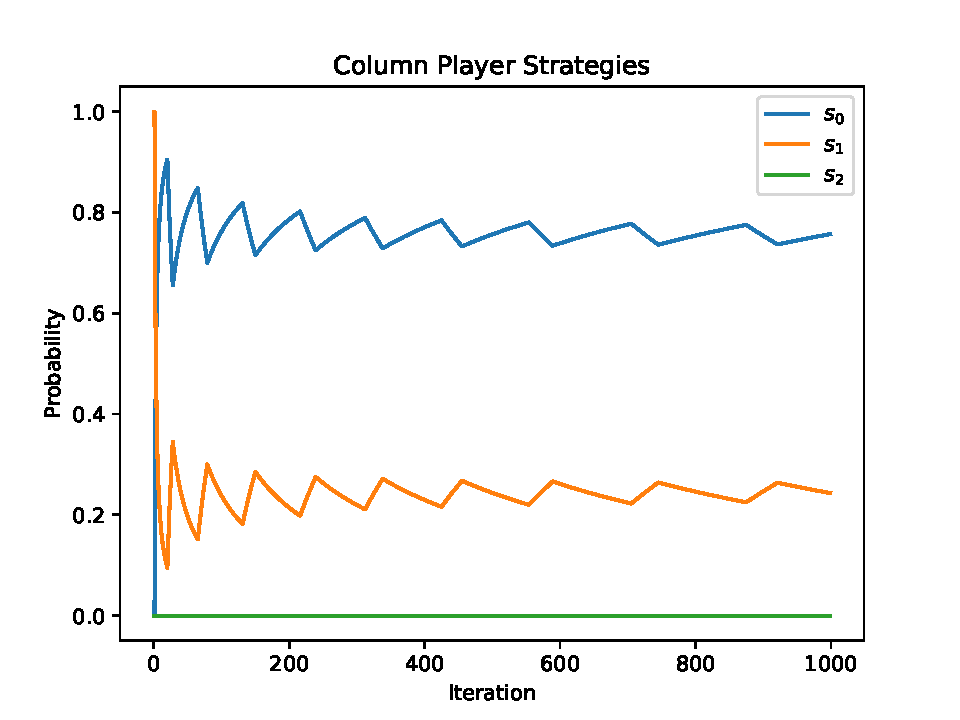
\includegraphics[width=0.45\textwidth]{chapters/04_game_theoretic_model/Bin/learning_algorithms_example/fictitious_col.pdf}
    \caption{Example of fictitious play algorithm run for \(1000\) iterations
    that converges to a Nash equilibrium.}
    \label{fig:fictitious_play}
\end{figure}


\subsubsection{Stochastic fictitious play}s
Another similar learning algorithm is called stochastic fictitious
play~\cite{hofbauerstochasticfictitous, fudenberg1998theory}.
Stochastic fictitious play is a variation of the fictitious play algorithm
where a stochastic perturbation \(\epsilon_i\) is added to each expected payoff
where \(\epsilon_i \in [0, \bar{\epsilon}]\) where \(\bar{\epsilon}\) is a
parameter needed for the algorithm.


\begin{lstlisting}[style=pystyle]
>>> A = np.array([
...     [4, 1, 3],
...     [2, 0, 2],
...     [3, 4, 1]
... ])
>>> B = np.array([
...     [4, 5, 1],
...     [2, 3, 2],
...     [6, 4, 0]
... ])
>>> game = nash.Game(A, B)
>>> np.random.seed(0)
>>> play_counts_and_distributions = tuple(
...     game.stochastic_fictitious_play(iterations=1000)
... )
>>> end_play_count, end_distribution = play_counts_and_distributions[-1]
>>> end_play_count
[array([624.,   0., 376.]), array([767., 233.,   0.])]

\end{lstlisting}

The output is the empirical probability of all actions played by player 1 and
player 2.
The outcome indicates that the stochastic fictitious play algorithm converges
to the following strategy: \(\sigma^1 = (\frac{2}{3}, 0, \frac{1}{3})\) and
\(\sigma^2 = (\frac{3}{4}, \frac{1}{4}, 0)\).
This is the outcome of the last iteration of the stochastic fictitious play
which is also similar to the fictitious play outcome.
Figure~\ref{fig:stochastic_fictitious_play} shows all iterations of the
stochastic fictitious play algorithm and how the players converge to a Nash
equilibrium.

\begin{figure}[H]
    \centering
    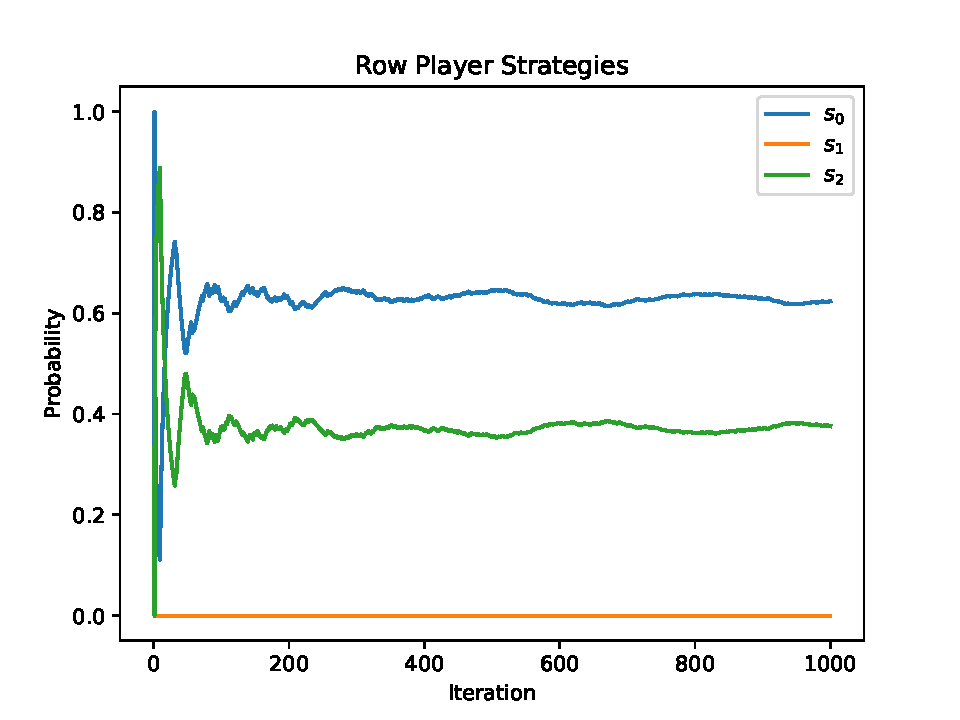
\includegraphics[width=0.45\textwidth]{chapters/04_game_theoretic_model/Bin/learning_algorithms_example/stochastic_row.pdf}
    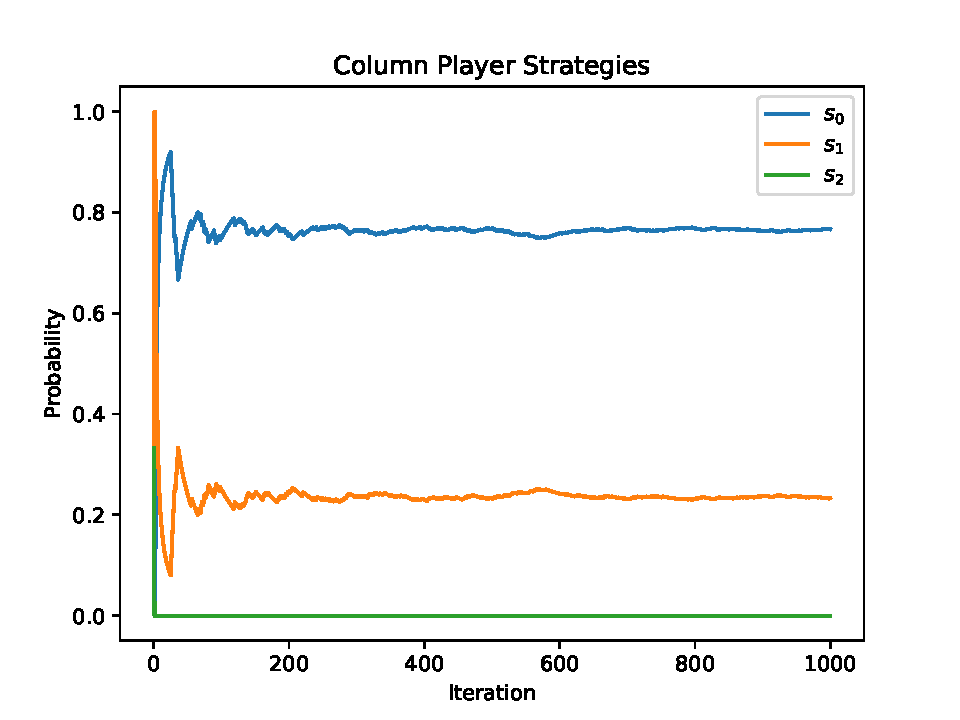
\includegraphics[width=0.45\textwidth]{chapters/04_game_theoretic_model/Bin/learning_algorithms_example/stochastic_col.pdf}
    \caption{Example of stochastic fictitious play algorithm for \(1000\)
    iterations that converges to a Nash equilibrium.}
    \label{fig:stochastic_fictitious_play}
\end{figure}


\subsubsection{Asymmetric replicator dynamics}

The learning algorithm that will be used most in this thesis is asymmetric
replicator dynamics~\cite{accinelli2011evolutionarily}.
Replicator dynamics is a learning algorithm that is used to express the
evolutionary dynamics of a population of players~\cite{komarova2004replicator}.
Consider a large population of some agents, also known as replicators.
Different types of such replicators meet and interact.
Each such interaction generates a certain payoff for each type of the
replicators.
This payoff is often referred to as the fitness of the replicator.
In evolutionary game theory these replicators are the strategies of the two
players.

Consider two types of individuals, \(A\) and \(B\), each with their own set of
strategies, \(S^A\) and \(S^B\).
Different strategies from \(S^A\) are assigned among the population of type
\(A\) and different strategies from \(S^B\) are assigned among the population
of type \(B\).
Individuals of type \(A\) are randomly paired with individuals of type \(B\)
and perform their assigned strategies.
As the game progresses the proportion of each strategy changes based on previous
interactions.
Given that the payoff matrices of the two players are \(A\) and \(B\), the
fitness of a strategy is given by:

\begin{equation}\label{eq:fitness_definition}
    f_x = A y \quad f_y = x^T B
\end{equation}

Note that \(x\) and \(y\) are the strategy vectors and correspond to the
population proportion of each strategy.
The average fitness of the two types of individuals is also given by:

\begin{equation}\label{eq:average_fitness_definition}
    \phi_x = f_x x^T \quad \phi_y = f_y y
\end{equation}

Finally the rate of change of the strategies are captured by the following
equations:

\begin{align}\label{eq:replicator_dynamics}
    \frac{dx}{dt} &= x_i((f_x)_i - \phi_x) \quad \text{for all } i \\
    \frac{dy}{dt} &= y_i((f_y)_i - \phi_y) \quad \text{for all } i
\end{align}

Asymmetric replicator dynamics is implemented by using the python
\lstinline[style=pystyle]{nashpy} library.
The following code snippet shows how to use the asymmetric replicator dynamics
algorithm to find the Nash equilibrium of a two-player game.
Consider the rock-paper-scissors game defined by the matrices
in~\eqref{eq:rock_paper_scissors_payoff}.

\begin{lstlisting}[style=pystyle]
>>> A = np.array([
...     [4, 1, 3],
...     [2, 0, 2],
...     [3, 4, 1]
... ])
>>> B = np.array([
...     [4, 5, 1],
...     [2, 3, 2],
...     [6, 4, 0]
... ])
>>> game = nash.Game(A, B)
>>> xs, ys = game.asymmetric_replicator_dynamics(
...     timepoints=np.linspace(0, 100, 100),
... )
>>> np.round(xs[-1], 4)
array([0.9207, 0.    , 0.0793])
>>> np.round(ys[-1], 4)
array([0.7429, 0.2571, 0.    ])

\end{lstlisting}

The output of the asymmetric replicator dynamics algorithm is the latest
population proportion of each strategy \(\sigma^1 = (0.92, 0, 0.08)\) and
\(\sigma^2 = (0.74, 0.25, 0)\).
That doesn't mean that the strategies have reached a steady state.
For this condition to be reached the rate of change of the strategies needs to
be \(\frac{dx}{dt} = \frac{dy}{dt} = 0\).
In fact Figure~\ref{fig:asymmetric_replicator_dynamics} shows that the
strategies played over time using the asymmetric replicator dynamics algorithm
have in fact not reached a steady state.

\begin{figure}[H]
    \centering
    \includegraphics[width=0.45\textwidth]{chapters/04_game_theoretic_model/Bin/learning_algorithms_example/asymmetric_rd_row.pdf}
    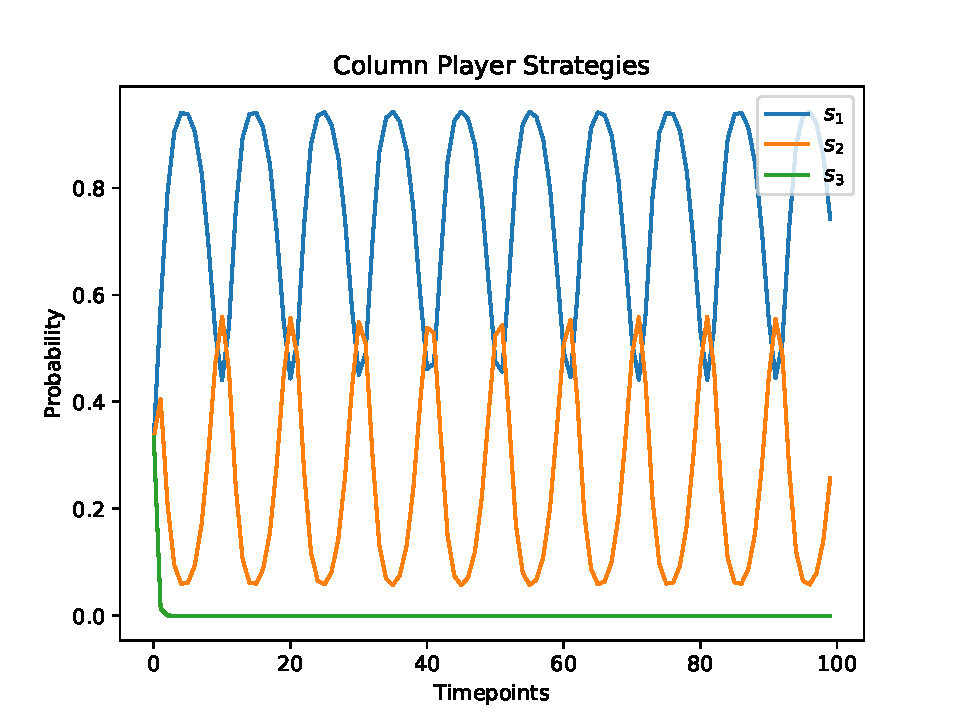
\includegraphics[width=0.45\textwidth]{chapters/04_game_theoretic_model/Bin/learning_algorithms_example/asymmetric_rd_col.pdf}
    \caption{Example of asymmetric replicator dynamics algorithm that does
    not converge.}
    \label{fig:asymmetric_replicator_dynamics}
\end{figure}

It can be seen that strategies player 1 alternates between strategy \(s_1\) and
\(s_3\) while player 2 alternates between strategy \(s_1\) and \(s_2\).
This game cannot reach a steady state given the uniform initial distribution of
the strategies.
Consider a different game where the steady strategy choice can be reached.

\begin{lstlisting}[style=pystyle]
>>> A = np.array([
...     [4, 1],
...     [2, 5],
... ])
>>> B = np.array([
...     [4, 5],
...     [2, 3],
... ])
>>> game = nash.Game(A, B)
>>> x0 = np.array([0.9, 0.1])
>>> y0 = np.array([0.9, 0.1])
>>> xs, ys = game.asymmetric_replicator_dynamics(
...     timepoints=np.linspace(0, 20, 100),
...     x0=x0,
...     y0=y0,
... )
>>> np.round(xs[-1], 4)
array([0., 1.])
>>> np.round(ys[-1], 4)
array([0., 1.])

\end{lstlisting}

The output of the asymmetric replicator dynamics algorithm is the latest
population proportion of each strategy \(\sigma^1 = (0, 1)\) and
\(\sigma^2 = (0, 1)\).
This indicates that the strategies have reached a steady state.
In replicator dynamics when a replicator is eliminated (in this case strategy
\(s_1\)), it cannot be recovered.
In addition, note that for this game the asymmetric replicator dynamics
algorithm was ran with a non-uniform initial distribution of the strategies.
In fact, even though the initial distribution of the strategies was
\(x_0 = (0.9, 0.1)\) and \(y_0 = (0.9, 0.1)\), strategy \(s_2\) still managed
to take over the population.

\begin{figure}[H]
    \centering
    \includegraphics[width=0.45\textwidth]{chapters/04_game_theoretic_model/Bin/learning_algorithms_example/asymmetric_rd_2_row.pdf}
    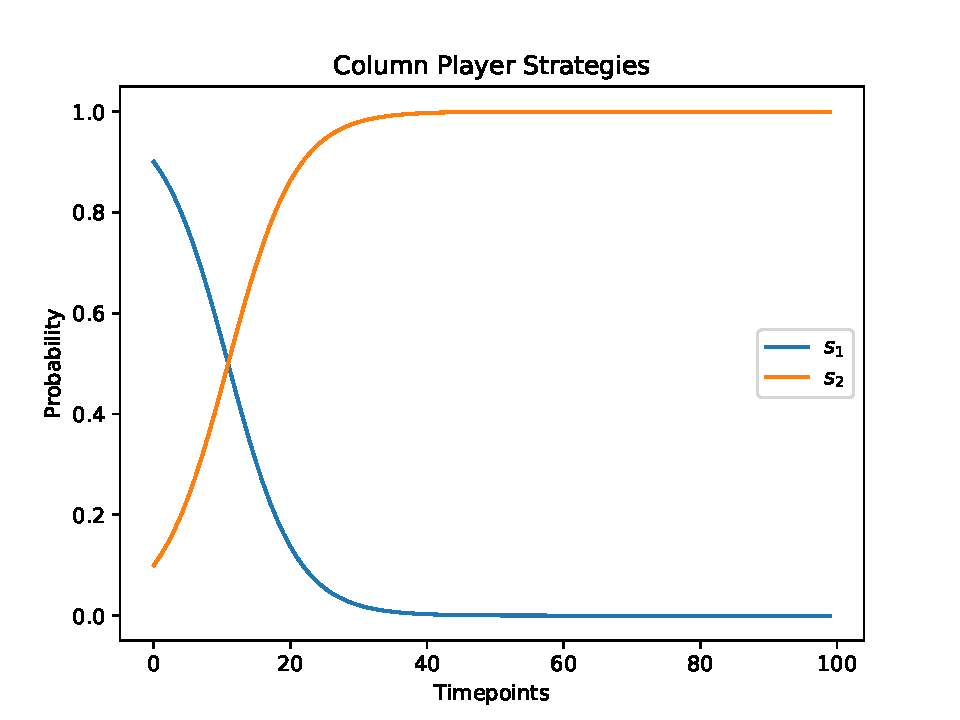
\includegraphics[width=0.45\textwidth]{chapters/04_game_theoretic_model/Bin/learning_algorithms_example/asymmetric_rd_2_col.pdf}
    \caption{Example of asymmetric replicator dynamics algorithm that converges}
    \label{fig:asymmetric_replicator_dynamics_steady}
\end{figure}


\subsection{Perfect-information extensive form game}

Unlike normal-form games extensive-form games work in a sequential way, where
players do not make decisions at the same time.
Instead, the first player chooses their strategy and then the opposing player,
fully aware of the choice made by the first player, chooses their own strategy.
There are numerous situations where decision makers can change their actions
based on the actions of other decision makers.
Such type of sequential games are also referred to as extensive form games.
One of the most common types of extensive form games is the perfect-information
extensive form game.
In this type of game, the players are assumed to have perfect information
about the previous actions of other
players.
There are four key components of a perfect-information extensive form game; the
players, the terminal nodes, the player function and the preferences of the
players~\cite{osborne2004_extensive_form_games}.
Examples of such games are the game of chess and the game of
Backgammon~\cite{hart1992games}.

Perfect information extensive form games are represented by a tree where the
nodes of the tree are the terminal nodes and represent the outcome of the
game.
The following figure shows an example of a perfect information extensive form
game.

\begin{figure}[H]
    \centering
    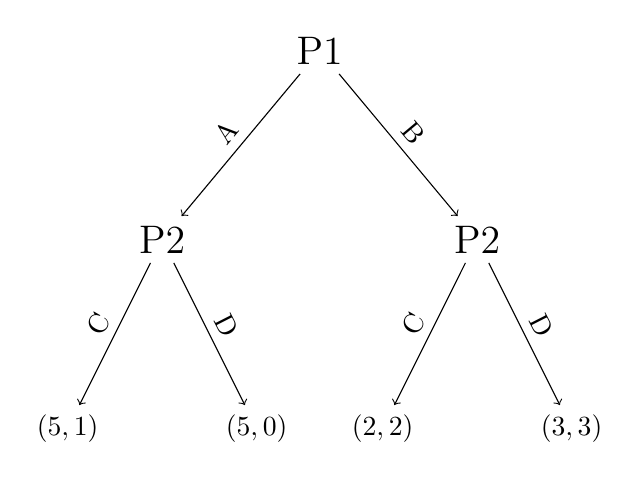
\begin{tikzpicture}[-, node distance = 2cm, scale=0.8]
    \node[anchor=north](P1){\Large{P1}};
    \node[anchor=north](P2_1) at (-2.5, -3) {\Large{P2}};
    \node[anchor=north](P2_2) at (2.5, -3) {\Large{P2}};

    \path[->] (P1) edge node [above, rotate=50] {A}(P2_1);
    \path[<-] (P2_2) edge node [above, rotate=310] {B}(P1);

    \node[anchor=north](F_1) at (-4, -6) {\((5,1)\)};
    \node[anchor=north](F_2) at (-1, -6) {\((5,0)\)};
    \node[anchor=north](F_3) at (1, -6) {\((2,2)\)};
    \node[anchor=north](F_4) at (4, -6) {\((3,3)\)};

    \path[->] (P2_1) edge node [above, rotate=60] {C}(F_1);
    \path[->] (P2_1) edge node [above, rotate=297] {D}(F_2);
    \path[->] (P2_2) edge node [above, rotate=60] {C}(F_3);
    \path[->] (P2_2) edge node [above, rotate=297] {D}(F_4);
\end{tikzpicture}

    \caption{Example of a perfect information extensive form game with \(2\)
    players and \(4\) terminal nodes.}
    \label{fig:extensive_form_game}
\end{figure}

Figure~\ref{fig:extensive_form_game} shows an example of a perfect information
extensive form game.
The game starts at the root node and the players take turns to make a move.
Player 1 can choose to either action A or action B.
Once player 1 has made a move, player 2 can choose to either action C or action
D, while having complete awareness of the action taken by player 1 and hence
their own position on the tree.
The final nodes of the tree represent the outcome of the game.
In this example, the outcome of the game is either 

\subsection{Imperfect-information extensive form game}
\label{sec:game_imperfect_information}

An imperfect information game is defined as an extensive form game where some
of the information about the game state is hidden for at least one of the
players~\cite{Berwanger2008}.
In other words, when making a decision, the players might not know their exact
position on the tree.
Similar to perfect information, imperfect information games are also represented
by a tree.
The following figure shows an example of an imperfect information extensive
form game.

\begin{figure}[H]
    \centering
    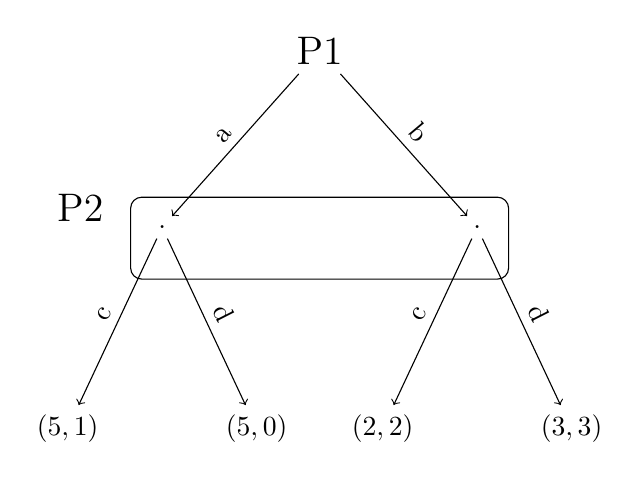
\begin{tikzpicture}[-, node distance = 2cm, scale=0.8]
    \node[anchor=north](P1){\Large{P1}};
    \node[anchor=north](P2_1) at (-2.5, -3) {.};
    \node[anchor=north](P2_2) at (2.5, -3) {.};
    \node[anchor=north](P2_3) at (-3.8, -2.5) {\Large{P2}};

    % \draw (0,-3.4) ellipse (3cm and 1cm);
    \draw[rounded corners] (-3, -4) rectangle (3, -2.7) {};

    \path[->] (P1) edge node [above, rotate=50] {a}(P2_1);
    \path[<-] (P2_2) edge node [above, rotate=310] {b}(P1);

    \node[anchor=north](F_1) at (-4, -6) {\((5,1)\)};
    \node[anchor=north](F_2) at (-1, -6) {\((5,0)\)};
    \node[anchor=north](F_3) at (1, -6) {\((2,2)\)};
    \node[anchor=north](F_4) at (4, -6) {\((3,3)\)};

    \path[->] (P2_1) edge node [above, rotate=60] {c}(F_1);
    \path[->] (P2_1) edge node [above, rotate=297] {d}(F_2);
    \path[->] (P2_2) edge node [above, rotate=60] {c}(F_3);
    \path[->] (P2_2) edge node [above, rotate=297] {d}(F_4);
\end{tikzpicture}

    \caption{An example of an imperfect information extensive form game with
    \(2\) players and \(4\) terminal nodes.}
    \label{fig:imperfect_extensive_form_game}
\end{figure}

Figure~\ref{fig:imperfect_extensive_form_game} shows an example of an imperfect
information extensive form game where player 2, when making their decision,
does not know whether they are in the left or right branch of the tree.
The game starts at the root node and the players take turns to make a move.
Player 1 can choose to either action \(a\) or action \(b\).
Once player 1 has made a move, player 2 can choose to either action \(c\) or
action \(d\), while having incomplete awareness of the action taken by player 1
and hence their own position on the tree.
The final nodes of the tree represent the outcome of the game.
This game can also be represented by a normal form game since both players end
up being completely unaware of the actions taken by the other player.
The payoff matrices in~\eqref{eq:imperfect_to_normal_form} show the normal form
game representation of the imperfect information extensive form game shown in
Figure~\ref{fig:imperfect_extensive_form_game}.
\begin{align}\label{eq:imperfect_to_normal_form}
    & \quad c \ \ d \nonumber \\
    A =
    \begin{matrix}
        a \\
        b
    \end{matrix}
    \begin{pmatrix}
        5 & 5 \\
        2 & 3
    \end{pmatrix} \quad
    B =&
    \begin{pmatrix}
        1 & 0 \\
        2 & 3
    \end{pmatrix}
\end{align}


\section{Formulation}\label{sec:game_formulation}

In order to formulate the game theoretic model one needs to define the players
of the game, the strategies of each player and the payoffs of each pair of
strategy being played.

\subsection{Players and parameters}\label{sec:game_players_and_parameters}

The problem studied is a 3-player extensive form game that consists of three
players.
This will later be reduced to a 2-player standard normal form
game~\cite{Maschler2013}.
The three players are:

\begin{itemize}
    \item the decision makers of queueing system \(A\)
    \item the decision makers of queueing system \(B\)
    \item a distribution service that distributes individuals to the two
    queueing systems
\end{itemize}

\begin{figure}[H]
    \centering
    \begin{minipage}{.3\textwidth}
    \raggedright
    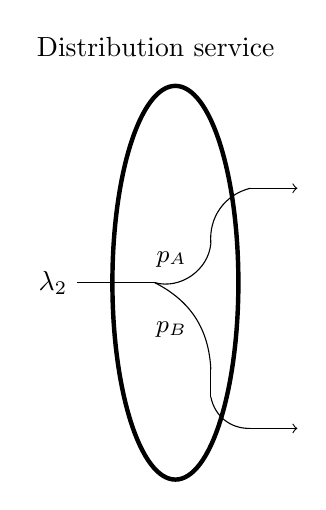
\begin{tikzpicture}
        \draw[ultra thick] (0.75,2) ellipse (0.8cm and 2.5cm);
        \node at (0.5, 5) {Distribution service};
        \draw[-] (0.5, 2) -- ++(-1, 0) node[left] {\(\lambda_2\)};

        % p_A line
        \path (0.49, 2) edge [bend right=50] (1.2, 2.5);
        \path (1.2, 2.5) edge [bend left=40] (1.7, 3.2);
        \draw[->] (1.7, 3.2) -- ++(0.6, 0.);

        % p_B line
        \path (0.49, 2) edge [bend left=30] (1.2, 0.9);
        \draw[-] (1.2, 0.9) -- (1.2, 0.55);
        \path (1.2, 0.55) edge [bend right=40] (1.7, 0.15);
        \draw[->] (1.7, 0.15) -- ++(0.6, 0.);

        \node at (0.7, 2.3) {\small{\( p_A \)}};
        \node at (0.7, 1.4) {\small{\( p_B \)}};
    \end{tikzpicture}
\end{minipage}
\begin{minipage}{.65\textwidth}
    \centering
    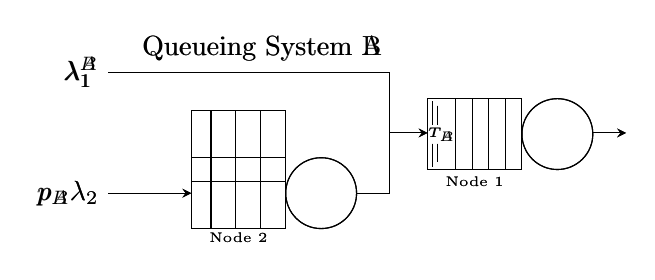
\begin{tikzpicture}[>=stealth, scale=0.6] %arrow type
        % Difference between the two queue diagrams
        
        \tikzmath{
            let \diff = -5cm;
        }
            
        % QUEUEING SYSTEM A

        \node at (1.5cm, 2.3cm) {Queueing System A};
            
        % the rectangle with vertical lines (Node 2)
        \draw (0,0) -- ++(2cm,0) -- ++(0,-1.5cm) -- ++(-2cm,0);
        \foreach \i in {1,...,3, 3.8}
        \draw (2cm-\i*15pt,0) -- +(0,-1.5cm);
        \node at (1, -1.7) {\tiny{Node 2}};

        % the circle (Node 2)
        \draw (2.75,-0.75cm) circle [radius=0.75cm];

        % the rectangle with vertical lines (Node 1)
        \draw (5,1.25) -- ++(2cm,0) -- ++(0,-1.5cm) -- ++(-2cm,0);
        \foreach \i in {1,...,4, 5.7}
        \draw (7cm-\i*10pt,1.25) -- +(0,-1.5cm);
        \node at (6, -0.5) {\tiny{Node 1}};

        % The two vertical lines at the start of Node 1
        \draw (7cm-54pt, 1.2cm) -- +(0,-0.5cm);
        \draw (7cm-54pt, 0.3cm) -- +(0,-0.5cm);
        \draw (7cm-51pt, 1.1cm) -- +(0,-0.4cm);
        \draw (7cm-51pt, 0.3cm) -- +(0,-0.4cm);

        % The label between the lines for T
        \node[anchor=north] at (5.3, 0.84) {\tiny{\( T_A \)}};

        % the circle (Node 1)
        \draw (7.75,0.5) circle [radius=0.75cm];

        % the arrows and labels (Node 2+2)
        \draw[->] (8.5,0.525) -- +(20pt,0);

        % Ambulance lines
        \draw[<-] (0,-0.75) -- +(-50pt,0) node[left] {\( p_A \lambda_2 \)};
        \draw[-] (3.5,-0.75) -- +(20pt,0);
        \draw (4.2, 0.525) -- (4.2, -0.75);

        % Others lines
        \draw (4.2, 1.8) -- +(-169.5pt,0) node[left] {\( \lambda_1^A \)};
        \draw (4.2, 1.8) -- (4.2, 0.525);
        \draw[->] (4.2, 0.525) -- (5, 0.525);


        % QUEUEING SYSTEM B

        \node at (1.5cm, \diff + 2.3cm) {Queueing System B};

        % the rectangle with vertical rules (Node 2)
        \draw (0, \diff) -- ++(2cm,0) -- ++(0,-1.5cm) -- ++(-2cm,0);
        \foreach \i in {1,...,3, 3.8}
        \draw (2cm-\i*15pt,\diff) -- +(0,-1.5cm);
        \node at (1cm, \diff - 1.7cm) {\tiny{Node 2}};

        % the circle (Node 2)
        \draw (2.75,\diff - 0.75cm) circle [radius=0.75cm];

        % the rectangle with vertical rules (Queue 2)
        \draw (5,\diff + 1.25cm) -- ++(2cm,0) -- ++(0,-1.5cm) -- ++(-2cm,0);
        \foreach \i in {1,...,4, 5.7}
        \draw (7cm-\i*10pt,\diff + 1.25cm) -- +(0,-1.5cm);
        \node at (6, \diff - 0.5cm) {\tiny{Node 1}};

        % The two vertical lines at the start of Queue 2
        \draw (7cm-54pt,\diff + 1.2cm) -- +(0,-0.5cm);
        \draw (7cm-54pt,\diff + 0.3cm) -- +(0,-0.5cm);
        \draw (7cm-51pt,\diff + 1.1cm) -- +(0,-0.4cm);
        \draw (7cm-51pt,\diff + 0.3cm) -- +(0,-0.4cm);

        % The label between the lines for T
        \node[anchor=north] at (5.3, \diff + 0.84cm) {\tiny{\( T_B \)}};

        % the circle (Queue 2)
        \draw (7.75,\diff + 0.5cm) circle [radius=0.75cm];

        % the arrows and labels (Node 2+2)
        \draw[->] (8.5, \diff + 0.525cm) -- +(20pt,0);

        % Ambulance lines
        \draw[<-] (0, \diff - 0.75cm) -- +(-50pt,0) node[left]
        {\( p_B \lambda_2 \)};
        \draw[-] (3.5, \diff - 0.75cm) -- +(20pt,0);
        \draw (4.2, \diff + 0.525cm) -- (4.2, \diff - 0.75cm);

        % Others lines
        \draw (4.2, \diff + 1.8cm) -- +(-169.5pt,0) node[left]
        {\( \lambda_1^B \)};
        \draw (4.2, \diff + 1.8cm) -- (4.2, \diff + 0.525);
        \draw[->] (4.2, \diff + 0.525cm) -- (5, \diff + 0.525cm);
    \end{tikzpicture}
\end{minipage}

    \caption{A diagrammatic representation of the game theoretic model.
    Individuals arrive at the distribution service at a rate of \( \lambda_2 \)
    and then a proportion of them are distributed to Queueing system \(A\)
    (\(p_A\)) and the remaining proportion to Queueing system \(B\) (\(p_B\))
    so that \(p_A + p_B = 1\).
    The corresponding arrival rates of type 2 individuals to Queueing systems
    \(A\) and \(B\) are thus given by:
    \( p_A \lambda_2 \) and \( p_B \lambda_2 \).}
    \label{fig:diagram_of_game_theoretic_model}
\end{figure}

Each player has their own objective which they aim to optimise.
More specifically, the queueing systems' objective is captured by an upper bound
of the time that a fixed proportion of individuals spend in the system,
while the distribution service aims to minimise the time that its individuals
stay blocked at each queueing system's node 2.
These objectives are more formally defined in Section~\ref{sec:game_strategies}.
The parameters of the game theoretic model are:

\begin{itemize}
    \item \(\lambda_2\): The arrival rate of type 2 individuals arriving at the
    distribution service that need to be distributed to the queueing systems
    \item \(\lambda_{1_i}\): The arrival rate of type 1 individuals to queueing
    system \(i\in\{A, B\}\)
    \item \(\mu_i\): The service rate of individuals at queueing system
    \(i\in\{A, B\}\)
    \item \(C_i\): The number of servers in queueing system \(i\in\{A, B\}\)
    \item \(T_i\): The strategy that queueing system \(i\in\{A, B\} \) chooses
    to play which corresponds to the threshold at which they start blocking
    type 2 individuals at node 2.
    \item \(N_i\): The total capacity of node 1 in queueing system
    \(i\in\{A, B\}\)
    \item \(M_i\): The total capacity of node 2 in queueing system
    \(i\in\{A, B\}\)
    \item \(t\): The time target for both queueing systems
    \item \(\alpha \in [0, 1]\) : Weighted average of blocking time and
    lost individuals (defined in equation~\eqref{eq:obj_distributor_penalty})
    \item \(\hat{P}\): is the percentage target of individuals that need to be
    within that target (this is set to 95\% unless otherwise stated)
\end{itemize}

\subsection{Strategies}\label{sec:game_strategies}

Each player is given a predetermined set of strategies from which to choose.
The strategies of the two queueing systems are the range of thresholds that they
can choose from.
In essence the strategy space of queueing system \(A\) is the set of integers
from
1 to the capacity of node 1 in queueing system \(A\) (\(N_A\)), while the
strategy space of queueing system \(B\) is the set of integers from 1 to the
capacity of node 1 in queueing system \(B\) (\(N_B\)).

\begin{equation}\label{eq:game_strategy_space_queueing_systems}
    T_A \in \{1, 2, \ldots, N_A\} \quad \text{and} \quad
    T_B \in \{1, 2, \ldots, N_B\}
\end{equation}

In essence this means that for either queueing system  (\(A\) or \(B\)), every
strategy
choice generates a different queueing network of the form that is described in
Section~\ref{sec:queueing_section}.
In other words, different strategies are equivalent to different thresholds
which is one of the core parameters of the queueing network.
Consider queueing system \(A\) as one of the three players of the game theoretic
model with node 1 capacity of \(N_A = 6\) and node 2 capacity of \(M_A = 3\).
The strategy space of queueing system \(A\) is then
\(T_A \in \{1, 2, 3, 4, 5, 6\}\).
Every possible value of \(T_A\) corresponds to a different queueing network.
Figures~\ref{fig:game_strategy_visualisation_N_6_M_3_first}
-~\ref{fig:game_strategy_visualisation_N_6_M_3_last} show all possible Markov chain
models that arise from such a strategy space.

\begin{figure}[H]
    \centering
    \scalebox{0.8}{
        \begin{tikzpicture}[-, node distance = 1cm, auto]
\node[state] (u0v0) {(0,0)};
\node[state, right=of u0v0] (u0v1) {(0,1)};
\draw[->](u0v0) edge[bend left] node {\( \Lambda \)} (u0v1);
\draw[->](u0v1) edge[bend left] node {\(\mu \)} (u0v0);
\node[state, below=of u0v1] (u1v1) {(1,1)};
\draw[->](u0v1) edge[bend left] node {\( \lambda_2 \)} (u1v1);
\draw[->](u1v1) edge[bend left] node {\(\mu \)} (u0v1);
\node[state, below=of u1v1] (u2v1) {(2,1)};
\draw[->](u1v1) edge[bend left] node {\( \lambda_2 \)} (u2v1);
\draw[->](u2v1) edge[bend left] node {\(\mu \)} (u1v1);
\node[state, below=of u2v1] (u3v1) {(3,1)};
\draw[->](u2v1) edge[bend left] node {\( \lambda_2 \)} (u3v1);
\draw[->](u3v1) edge[bend left] node {\(\mu \)} (u2v1);
\node[state, right=of u0v1] (u0v2) {(0,2)};
\draw[->](u0v1) edge[bend left] node {\( \lambda_1 \)} (u0v2);
\draw[->](u0v2) edge[bend left] node {\(\mu \)} (u0v1);
\node[state, right=of u1v1] (u1v2) {(1,2)};
\draw[->](u1v1) edge[bend left] node {\( \lambda_1 \)} (u1v2);
\draw[->](u1v2) edge[bend left] node {\(\mu \)} (u1v1);
\draw[->](u0v2) edge node {\( \lambda_2 \)} (u1v2);
\node[state, right=of u2v1] (u2v2) {(2,2)};
\draw[->](u2v1) edge[bend left] node {\( \lambda_1 \)} (u2v2);
\draw[->](u2v2) edge[bend left] node {\(\mu \)} (u2v1);
\draw[->](u1v2) edge node {\( \lambda_2 \)} (u2v2);
\node[state, right=of u3v1] (u3v2) {(3,2)};
\draw[->](u3v1) edge[bend left] node {\( \lambda_1 \)} (u3v2);
\draw[->](u3v2) edge[bend left] node {\(\mu \)} (u3v1);
\draw[->](u2v2) edge node {\( \lambda_2 \)} (u3v2);
\node[state, right=of u0v2] (u0v3) {(0,3)};
\draw[->](u0v2) edge[bend left] node {\( \lambda_1 \)} (u0v3);
\draw[->](u0v3) edge[bend left] node {\(\mu \)} (u0v2);
\node[state, right=of u1v2] (u1v3) {(1,3)};
\draw[->](u1v2) edge[bend left] node {\( \lambda_1 \)} (u1v3);
\draw[->](u1v3) edge[bend left] node {\(\mu \)} (u1v2);
\draw[->](u0v3) edge node {\( \lambda_2 \)} (u1v3);
\node[state, right=of u2v2] (u2v3) {(2,3)};
\draw[->](u2v2) edge[bend left] node {\( \lambda_1 \)} (u2v3);
\draw[->](u2v3) edge[bend left] node {\(\mu \)} (u2v2);
\draw[->](u1v3) edge node {\( \lambda_2 \)} (u2v3);
\node[state, right=of u3v2] (u3v3) {(3,3)};
\draw[->](u3v2) edge[bend left] node {\( \lambda_1 \)} (u3v3);
\draw[->](u3v3) edge[bend left] node {\(\mu \)} (u3v2);
\draw[->](u2v3) edge node {\( \lambda_2 \)} (u3v3);
\node[state, right=of u0v3] (u0v4) {(0,4)};
\draw[->](u0v3) edge[bend left] node {\( \lambda_1 \)} (u0v4);
\draw[->](u0v4) edge[bend left] node {\(\mu \)} (u0v3);
\node[state, right=of u1v3] (u1v4) {(1,4)};
\draw[->](u1v3) edge[bend left] node {\( \lambda_1 \)} (u1v4);
\draw[->](u1v4) edge[bend left] node {\(\mu \)} (u1v3);
\draw[->](u0v4) edge node {\( \lambda_2 \)} (u1v4);
\node[state, right=of u2v3] (u2v4) {(2,4)};
\draw[->](u2v3) edge[bend left] node {\( \lambda_1 \)} (u2v4);
\draw[->](u2v4) edge[bend left] node {\(\mu \)} (u2v3);
\draw[->](u1v4) edge node {\( \lambda_2 \)} (u2v4);
\node[state, right=of u3v3] (u3v4) {(3,4)};
\draw[->](u3v3) edge[bend left] node {\( \lambda_1 \)} (u3v4);
\draw[->](u3v4) edge[bend left] node {\(\mu \)} (u3v3);
\draw[->](u2v4) edge node {\( \lambda_2 \)} (u3v4);
\node[state, right=of u0v4] (u0v5) {(0,5)};
\draw[->](u0v4) edge[bend left] node {\( \lambda_1 \)} (u0v5);
\draw[->](u0v5) edge[bend left] node {\(\mu \)} (u0v4);
\node[state, right=of u1v4] (u1v5) {(1,5)};
\draw[->](u1v4) edge[bend left] node {\( \lambda_1 \)} (u1v5);
\draw[->](u1v5) edge[bend left] node {\(\mu \)} (u1v4);
\draw[->](u0v5) edge node {\( \lambda_2 \)} (u1v5);
\node[state, right=of u2v4] (u2v5) {(2,5)};
\draw[->](u2v4) edge[bend left] node {\( \lambda_1 \)} (u2v5);
\draw[->](u2v5) edge[bend left] node {\(\mu \)} (u2v4);
\draw[->](u1v5) edge node {\( \lambda_2 \)} (u2v5);
\node[state, right=of u3v4] (u3v5) {(3,5)};
\draw[->](u3v4) edge[bend left] node {\( \lambda_1 \)} (u3v5);
\draw[->](u3v5) edge[bend left] node {\(\mu \)} (u3v4);
\draw[->](u2v5) edge node {\( \lambda_2 \)} (u3v5);
\node[state, right=of u0v5] (u0v6) {(0,6)};
\draw[->](u0v5) edge[bend left] node {\( \lambda_1 \)} (u0v6);
\draw[->](u0v6) edge[bend left] node {\(\mu \)} (u0v5);
\node[state, right=of u1v5] (u1v6) {(1,6)};
\draw[->](u1v5) edge[bend left] node {\( \lambda_1 \)} (u1v6);
\draw[->](u1v6) edge[bend left] node {\(\mu \)} (u1v5);
\draw[->](u0v6) edge node {\( \lambda_2 \)} (u1v6);
\node[state, right=of u2v5] (u2v6) {(2,6)};
\draw[->](u2v5) edge[bend left] node {\( \lambda_1 \)} (u2v6);
\draw[->](u2v6) edge[bend left] node {\(\mu \)} (u2v5);
\draw[->](u1v6) edge node {\( \lambda_2 \)} (u2v6);
\node[state, right=of u3v5] (u3v6) {(3,6)};
\draw[->](u3v5) edge[bend left] node {\( \lambda_1 \)} (u3v6);
\draw[->](u3v6) edge[bend left] node {\(\mu \)} (u3v5);
\draw[->](u2v6) edge node {\( \lambda_2 \)} (u3v6);
\end{tikzpicture}
    }
    \caption{The Markov chain model that will be generated when queueing system
    \(A\) chooses to play a strategy of \(T_A = 1\).}
    \label{fig:game_strategy_visualisation_N_6_M_3_first}
\end{figure}

\begin{figure}[H]
    \centering
    \scalebox{0.8}{
        \begin{tikzpicture}[-, node distance = 1cm, auto]
\node[state] (u0v0) {(0,0)};
\node[state, right=of u0v0] (u0v1) {(0,1)};
\draw[->](u0v0) edge[bend left] node {\( \Lambda \)} (u0v1);
\draw[->](u0v1) edge[bend left] node {\(\mu \)} (u0v0);
\node[state, right=of u0v1] (u0v2) {(0,2)};
\draw[->](u0v1) edge[bend left] node {\( \Lambda \)} (u0v2);
\draw[->](u0v2) edge[bend left] node {\(\mu \)} (u0v1);
\node[state, below=of u0v2] (u1v2) {(1,2)};
\draw[->](u0v2) edge[bend left] node {\( \lambda_2 \)} (u1v2);
\draw[->](u1v2) edge[bend left] node {\(\mu \)} (u0v2);
\node[state, below=of u1v2] (u2v2) {(2,2)};
\draw[->](u1v2) edge[bend left] node {\( \lambda_2 \)} (u2v2);
\draw[->](u2v2) edge[bend left] node {\(\mu \)} (u1v2);
\node[state, below=of u2v2] (u3v2) {(3,2)};
\draw[->](u2v2) edge[bend left] node {\( \lambda_2 \)} (u3v2);
\draw[->](u3v2) edge[bend left] node {\(\mu \)} (u2v2);
\node[state, right=of u0v2] (u0v3) {(0,3)};
\draw[->](u0v2) edge[bend left] node {\( \lambda_1 \)} (u0v3);
\draw[->](u0v3) edge[bend left] node {\(\mu \)} (u0v2);
\node[state, right=of u1v2] (u1v3) {(1,3)};
\draw[->](u1v2) edge[bend left] node {\( \lambda_1 \)} (u1v3);
\draw[->](u1v3) edge[bend left] node {\(\mu \)} (u1v2);
\draw[->](u0v3) edge node {\( \lambda_2 \)} (u1v3);
\node[state, right=of u2v2] (u2v3) {(2,3)};
\draw[->](u2v2) edge[bend left] node {\( \lambda_1 \)} (u2v3);
\draw[->](u2v3) edge[bend left] node {\(\mu \)} (u2v2);
\draw[->](u1v3) edge node {\( \lambda_2 \)} (u2v3);
\node[state, right=of u3v2] (u3v3) {(3,3)};
\draw[->](u3v2) edge[bend left] node {\( \lambda_1 \)} (u3v3);
\draw[->](u3v3) edge[bend left] node {\(\mu \)} (u3v2);
\draw[->](u2v3) edge node {\( \lambda_2 \)} (u3v3);
\node[state, right=of u0v3] (u0v4) {(0,4)};
\draw[->](u0v3) edge[bend left] node {\( \lambda_1 \)} (u0v4);
\draw[->](u0v4) edge[bend left] node {\(\mu \)} (u0v3);
\node[state, right=of u1v3] (u1v4) {(1,4)};
\draw[->](u1v3) edge[bend left] node {\( \lambda_1 \)} (u1v4);
\draw[->](u1v4) edge[bend left] node {\(\mu \)} (u1v3);
\draw[->](u0v4) edge node {\( \lambda_2 \)} (u1v4);
\node[state, right=of u2v3] (u2v4) {(2,4)};
\draw[->](u2v3) edge[bend left] node {\( \lambda_1 \)} (u2v4);
\draw[->](u2v4) edge[bend left] node {\(\mu \)} (u2v3);
\draw[->](u1v4) edge node {\( \lambda_2 \)} (u2v4);
\node[state, right=of u3v3] (u3v4) {(3,4)};
\draw[->](u3v3) edge[bend left] node {\( \lambda_1 \)} (u3v4);
\draw[->](u3v4) edge[bend left] node {\(\mu \)} (u3v3);
\draw[->](u2v4) edge node {\( \lambda_2 \)} (u3v4);
\node[state, right=of u0v4] (u0v5) {(0,5)};
\draw[->](u0v4) edge[bend left] node {\( \lambda_1 \)} (u0v5);
\draw[->](u0v5) edge[bend left] node {\(\mu \)} (u0v4);
\node[state, right=of u1v4] (u1v5) {(1,5)};
\draw[->](u1v4) edge[bend left] node {\( \lambda_1 \)} (u1v5);
\draw[->](u1v5) edge[bend left] node {\(\mu \)} (u1v4);
\draw[->](u0v5) edge node {\( \lambda_2 \)} (u1v5);
\node[state, right=of u2v4] (u2v5) {(2,5)};
\draw[->](u2v4) edge[bend left] node {\( \lambda_1 \)} (u2v5);
\draw[->](u2v5) edge[bend left] node {\(\mu \)} (u2v4);
\draw[->](u1v5) edge node {\( \lambda_2 \)} (u2v5);
\node[state, right=of u3v4] (u3v5) {(3,5)};
\draw[->](u3v4) edge[bend left] node {\( \lambda_1 \)} (u3v5);
\draw[->](u3v5) edge[bend left] node {\(\mu \)} (u3v4);
\draw[->](u2v5) edge node {\( \lambda_2 \)} (u3v5);
\node[state, right=of u0v5] (u0v6) {(0,6)};
\draw[->](u0v5) edge[bend left] node {\( \lambda_1 \)} (u0v6);
\draw[->](u0v6) edge[bend left] node {\(\mu \)} (u0v5);
\node[state, right=of u1v5] (u1v6) {(1,6)};
\draw[->](u1v5) edge[bend left] node {\( \lambda_1 \)} (u1v6);
\draw[->](u1v6) edge[bend left] node {\(\mu \)} (u1v5);
\draw[->](u0v6) edge node {\( \lambda_2 \)} (u1v6);
\node[state, right=of u2v5] (u2v6) {(2,6)};
\draw[->](u2v5) edge[bend left] node {\( \lambda_1 \)} (u2v6);
\draw[->](u2v6) edge[bend left] node {\(\mu \)} (u2v5);
\draw[->](u1v6) edge node {\( \lambda_2 \)} (u2v6);
\node[state, right=of u3v5] (u3v6) {(3,6)};
\draw[->](u3v5) edge[bend left] node {\( \lambda_1 \)} (u3v6);
\draw[->](u3v6) edge[bend left] node {\(\mu \)} (u3v5);
\draw[->](u2v6) edge node {\( \lambda_2 \)} (u3v6);
\end{tikzpicture}
    }
    \caption{The Markov chain model that will be generated when queueing system
    \(A\) chooses to play a strategy of \(T_A = 2\).}
\end{figure}

\begin{figure}[H]
    \centering
    \scalebox{0.8}{
        \begin{tikzpicture}[-, node distance = 1cm, auto]
\node[state] (u0v0) {(0,0)};
\node[state, right=of u0v0] (u0v1) {(0,1)};
\draw[->](u0v0) edge[bend left] node {\( \Lambda \)} (u0v1);
\draw[->](u0v1) edge[bend left] node {\(\mu \)} (u0v0);
\node[state, right=of u0v1] (u0v2) {(0,2)};
\draw[->](u0v1) edge[bend left] node {\( \Lambda \)} (u0v2);
\draw[->](u0v2) edge[bend left] node {\(\mu \)} (u0v1);
\node[state, right=of u0v2] (u0v3) {(0,3)};
\draw[->](u0v2) edge[bend left] node {\( \Lambda \)} (u0v3);
\draw[->](u0v3) edge[bend left] node {\(\mu \)} (u0v2);
\node[state, below=of u0v3] (u1v3) {(1,3)};
\draw[->](u0v3) edge[bend left] node {\( \lambda_2 \)} (u1v3);
\draw[->](u1v3) edge[bend left] node {\(\mu \)} (u0v3);
\node[state, below=of u1v3] (u2v3) {(2,3)};
\draw[->](u1v3) edge[bend left] node {\( \lambda_2 \)} (u2v3);
\draw[->](u2v3) edge[bend left] node {\(\mu \)} (u1v3);
\node[state, below=of u2v3] (u3v3) {(3,3)};
\draw[->](u2v3) edge[bend left] node {\( \lambda_2 \)} (u3v3);
\draw[->](u3v3) edge[bend left] node {\(\mu \)} (u2v3);
\node[state, right=of u0v3] (u0v4) {(0,4)};
\draw[->](u0v3) edge[bend left] node {\( \lambda_1 \)} (u0v4);
\draw[->](u0v4) edge[bend left] node {\(\mu \)} (u0v3);
\node[state, right=of u1v3] (u1v4) {(1,4)};
\draw[->](u1v3) edge[bend left] node {\( \lambda_1 \)} (u1v4);
\draw[->](u1v4) edge[bend left] node {\(\mu \)} (u1v3);
\draw[->](u0v4) edge node {\( \lambda_2 \)} (u1v4);
\node[state, right=of u2v3] (u2v4) {(2,4)};
\draw[->](u2v3) edge[bend left] node {\( \lambda_1 \)} (u2v4);
\draw[->](u2v4) edge[bend left] node {\(\mu \)} (u2v3);
\draw[->](u1v4) edge node {\( \lambda_2 \)} (u2v4);
\node[state, right=of u3v3] (u3v4) {(3,4)};
\draw[->](u3v3) edge[bend left] node {\( \lambda_1 \)} (u3v4);
\draw[->](u3v4) edge[bend left] node {\(\mu \)} (u3v3);
\draw[->](u2v4) edge node {\( \lambda_2 \)} (u3v4);
\node[state, right=of u0v4] (u0v5) {(0,5)};
\draw[->](u0v4) edge[bend left] node {\( \lambda_1 \)} (u0v5);
\draw[->](u0v5) edge[bend left] node {\(\mu \)} (u0v4);
\node[state, right=of u1v4] (u1v5) {(1,5)};
\draw[->](u1v4) edge[bend left] node {\( \lambda_1 \)} (u1v5);
\draw[->](u1v5) edge[bend left] node {\(\mu \)} (u1v4);
\draw[->](u0v5) edge node {\( \lambda_2 \)} (u1v5);
\node[state, right=of u2v4] (u2v5) {(2,5)};
\draw[->](u2v4) edge[bend left] node {\( \lambda_1 \)} (u2v5);
\draw[->](u2v5) edge[bend left] node {\(\mu \)} (u2v4);
\draw[->](u1v5) edge node {\( \lambda_2 \)} (u2v5);
\node[state, right=of u3v4] (u3v5) {(3,5)};
\draw[->](u3v4) edge[bend left] node {\( \lambda_1 \)} (u3v5);
\draw[->](u3v5) edge[bend left] node {\(\mu \)} (u3v4);
\draw[->](u2v5) edge node {\( \lambda_2 \)} (u3v5);
\node[state, right=of u0v5] (u0v6) {(0,6)};
\draw[->](u0v5) edge[bend left] node {\( \lambda_1 \)} (u0v6);
\draw[->](u0v6) edge[bend left] node {\(\mu \)} (u0v5);
\node[state, right=of u1v5] (u1v6) {(1,6)};
\draw[->](u1v5) edge[bend left] node {\( \lambda_1 \)} (u1v6);
\draw[->](u1v6) edge[bend left] node {\(\mu \)} (u1v5);
\draw[->](u0v6) edge node {\( \lambda_2 \)} (u1v6);
\node[state, right=of u2v5] (u2v6) {(2,6)};
\draw[->](u2v5) edge[bend left] node {\( \lambda_1 \)} (u2v6);
\draw[->](u2v6) edge[bend left] node {\(\mu \)} (u2v5);
\draw[->](u1v6) edge node {\( \lambda_2 \)} (u2v6);
\node[state, right=of u3v5] (u3v6) {(3,6)};
\draw[->](u3v5) edge[bend left] node {\( \lambda_1 \)} (u3v6);
\draw[->](u3v6) edge[bend left] node {\(\mu \)} (u3v5);
\draw[->](u2v6) edge node {\( \lambda_2 \)} (u3v6);
\end{tikzpicture}
    }
    \caption{The Markov chain model that will be generated when queueing system
    \(A\) chooses to play a strategy of \(T_A = 3\).}
\end{figure}


\begin{figure}[H]
    \centering
    \scalebox{0.8}{
        \begin{tikzpicture}[-, node distance = 1cm, auto]
\node[state] (u0v0) {(0,0)};
\node[state, right=of u0v0] (u0v1) {(0,1)};
\draw[->](u0v0) edge[bend left] node {\( \Lambda \)} (u0v1);
\draw[->](u0v1) edge[bend left] node {\(\mu \)} (u0v0);
\node[state, right=of u0v1] (u0v2) {(0,2)};
\draw[->](u0v1) edge[bend left] node {\( \Lambda \)} (u0v2);
\draw[->](u0v2) edge[bend left] node {\(\mu \)} (u0v1);
\node[state, right=of u0v2] (u0v3) {(0,3)};
\draw[->](u0v2) edge[bend left] node {\( \Lambda \)} (u0v3);
\draw[->](u0v3) edge[bend left] node {\(\mu \)} (u0v2);
\node[state, right=of u0v3] (u0v4) {(0,4)};
\draw[->](u0v3) edge[bend left] node {\( \Lambda \)} (u0v4);
\draw[->](u0v4) edge[bend left] node {\(\mu \)} (u0v3);
\node[state, below=of u0v4] (u1v4) {(1,4)};
\draw[->](u0v4) edge[bend left] node {\( \lambda_2 \)} (u1v4);
\draw[->](u1v4) edge[bend left] node {\(\mu \)} (u0v4);
\node[state, below=of u1v4] (u2v4) {(2,4)};
\draw[->](u1v4) edge[bend left] node {\( \lambda_2 \)} (u2v4);
\draw[->](u2v4) edge[bend left] node {\(\mu \)} (u1v4);
\node[state, below=of u2v4] (u3v4) {(3,4)};
\draw[->](u2v4) edge[bend left] node {\( \lambda_2 \)} (u3v4);
\draw[->](u3v4) edge[bend left] node {\(\mu \)} (u2v4);
\node[state, right=of u0v4] (u0v5) {(0,5)};
\draw[->](u0v4) edge[bend left] node {\( \lambda_1 \)} (u0v5);
\draw[->](u0v5) edge[bend left] node {\(\mu \)} (u0v4);
\node[state, right=of u1v4] (u1v5) {(1,5)};
\draw[->](u1v4) edge[bend left] node {\( \lambda_1 \)} (u1v5);
\draw[->](u1v5) edge[bend left] node {\(\mu \)} (u1v4);
\draw[->](u0v5) edge node {\( \lambda_2 \)} (u1v5);
\node[state, right=of u2v4] (u2v5) {(2,5)};
\draw[->](u2v4) edge[bend left] node {\( \lambda_1 \)} (u2v5);
\draw[->](u2v5) edge[bend left] node {\(\mu \)} (u2v4);
\draw[->](u1v5) edge node {\( \lambda_2 \)} (u2v5);
\node[state, right=of u3v4] (u3v5) {(3,5)};
\draw[->](u3v4) edge[bend left] node {\( \lambda_1 \)} (u3v5);
\draw[->](u3v5) edge[bend left] node {\(\mu \)} (u3v4);
\draw[->](u2v5) edge node {\( \lambda_2 \)} (u3v5);
\node[state, right=of u0v5] (u0v6) {(0,6)};
\draw[->](u0v5) edge[bend left] node {\( \lambda_1 \)} (u0v6);
\draw[->](u0v6) edge[bend left] node {\(\mu \)} (u0v5);
\node[state, right=of u1v5] (u1v6) {(1,6)};
\draw[->](u1v5) edge[bend left] node {\( \lambda_1 \)} (u1v6);
\draw[->](u1v6) edge[bend left] node {\(\mu \)} (u1v5);
\draw[->](u0v6) edge node {\( \lambda_2 \)} (u1v6);
\node[state, right=of u2v5] (u2v6) {(2,6)};
\draw[->](u2v5) edge[bend left] node {\( \lambda_1 \)} (u2v6);
\draw[->](u2v6) edge[bend left] node {\(\mu \)} (u2v5);
\draw[->](u1v6) edge node {\( \lambda_2 \)} (u2v6);
\node[state, right=of u3v5] (u3v6) {(3,6)};
\draw[->](u3v5) edge[bend left] node {\( \lambda_1 \)} (u3v6);
\draw[->](u3v6) edge[bend left] node {\(\mu \)} (u3v5);
\draw[->](u2v6) edge node {\( \lambda_2 \)} (u3v6);
\end{tikzpicture}
    }
    \caption{The Markov chain model that will be generated when queueing system
    \(A\) chooses to play a strategy of \(T_A = 4\).}
\end{figure}

\begin{figure}[H]
    \centering
    \scalebox{0.8}{
        \begin{tikzpicture}[-, node distance = 1cm, auto]
\node[state] (u0v0) {(0,0)};
\node[state, right=of u0v0] (u0v1) {(0,1)};
\draw[->](u0v0) edge[bend left] node {\( \Lambda \)} (u0v1);
\draw[->](u0v1) edge[bend left] node {\(\mu \)} (u0v0);
\node[state, right=of u0v1] (u0v2) {(0,2)};
\draw[->](u0v1) edge[bend left] node {\( \Lambda \)} (u0v2);
\draw[->](u0v2) edge[bend left] node {\(\mu \)} (u0v1);
\node[state, right=of u0v2] (u0v3) {(0,3)};
\draw[->](u0v2) edge[bend left] node {\( \Lambda \)} (u0v3);
\draw[->](u0v3) edge[bend left] node {\(\mu \)} (u0v2);
\node[state, right=of u0v3] (u0v4) {(0,4)};
\draw[->](u0v3) edge[bend left] node {\( \Lambda \)} (u0v4);
\draw[->](u0v4) edge[bend left] node {\(\mu \)} (u0v3);
\node[state, right=of u0v4] (u0v5) {(0,5)};
\draw[->](u0v4) edge[bend left] node {\( \Lambda \)} (u0v5);
\draw[->](u0v5) edge[bend left] node {\(\mu \)} (u0v4);
\node[state, below=of u0v5] (u1v5) {(1,5)};
\draw[->](u0v5) edge[bend left] node {\( \lambda_2 \)} (u1v5);
\draw[->](u1v5) edge[bend left] node {\(\mu \)} (u0v5);
\node[state, below=of u1v5] (u2v5) {(2,5)};
\draw[->](u1v5) edge[bend left] node {\( \lambda_2 \)} (u2v5);
\draw[->](u2v5) edge[bend left] node {\(\mu \)} (u1v5);
\node[state, below=of u2v5] (u3v5) {(3,5)};
\draw[->](u2v5) edge[bend left] node {\( \lambda_2 \)} (u3v5);
\draw[->](u3v5) edge[bend left] node {\(\mu \)} (u2v5);
\node[state, right=of u0v5] (u0v6) {(0,6)};
\draw[->](u0v5) edge[bend left] node {\( \lambda_1 \)} (u0v6);
\draw[->](u0v6) edge[bend left] node {\(\mu \)} (u0v5);
\node[state, right=of u1v5] (u1v6) {(1,6)};
\draw[->](u1v5) edge[bend left] node {\( \lambda_1 \)} (u1v6);
\draw[->](u1v6) edge[bend left] node {\(\mu \)} (u1v5);
\draw[->](u0v6) edge node {\( \lambda_2 \)} (u1v6);
\node[state, right=of u2v5] (u2v6) {(2,6)};
\draw[->](u2v5) edge[bend left] node {\( \lambda_1 \)} (u2v6);
\draw[->](u2v6) edge[bend left] node {\(\mu \)} (u2v5);
\draw[->](u1v6) edge node {\( \lambda_2 \)} (u2v6);
\node[state, right=of u3v5] (u3v6) {(3,6)};
\draw[->](u3v5) edge[bend left] node {\( \lambda_1 \)} (u3v6);
\draw[->](u3v6) edge[bend left] node {\(\mu \)} (u3v5);
\draw[->](u2v6) edge node {\( \lambda_2 \)} (u3v6);
\end{tikzpicture}
    }
    \caption{The Markov chain model that will be generated when queueing system
    \(A\) chooses to play a strategy of \(T_A = 5\).}
\end{figure}

\begin{figure}[H]
    \centering
    \scalebox{0.8}{
        \begin{tikzpicture}[-, node distance = 1cm, auto]
\node[state] (u0v0) {(0,0)};
\node[state, right=of u0v0] (u0v1) {(0,1)};
\draw[->](u0v0) edge[bend left] node {\( \Lambda \)} (u0v1);
\draw[->](u0v1) edge[bend left] node {\(\mu \)} (u0v0);
\node[state, right=of u0v1] (u0v2) {(0,2)};
\draw[->](u0v1) edge[bend left] node {\( \Lambda \)} (u0v2);
\draw[->](u0v2) edge[bend left] node {\(\mu \)} (u0v1);
\node[state, right=of u0v2] (u0v3) {(0,3)};
\draw[->](u0v2) edge[bend left] node {\( \Lambda \)} (u0v3);
\draw[->](u0v3) edge[bend left] node {\(\mu \)} (u0v2);
\node[state, right=of u0v3] (u0v4) {(0,4)};
\draw[->](u0v3) edge[bend left] node {\( \Lambda \)} (u0v4);
\draw[->](u0v4) edge[bend left] node {\(\mu \)} (u0v3);
\node[state, right=of u0v4] (u0v5) {(0,5)};
\draw[->](u0v4) edge[bend left] node {\( \Lambda \)} (u0v5);
\draw[->](u0v5) edge[bend left] node {\(\mu \)} (u0v4);
\node[state, right=of u0v5] (u0v6) {(0,6)};
\draw[->](u0v5) edge[bend left] node {\( \Lambda \)} (u0v6);
\draw[->](u0v6) edge[bend left] node {\(\mu \)} (u0v5);
\node[state, below=of u0v6] (u1v6) {(1,6)};
\draw[->](u0v6) edge[bend left] node {\( \lambda_2 \)} (u1v6);
\draw[->](u1v6) edge[bend left] node {\(\mu \)} (u0v6);
\node[state, below=of u1v6] (u2v6) {(2,6)};
\draw[->](u1v6) edge[bend left] node {\( \lambda_2 \)} (u2v6);
\draw[->](u2v6) edge[bend left] node {\(\mu \)} (u1v6);
\node[state, below=of u2v6] (u3v6) {(3,6)};
\draw[->](u2v6) edge[bend left] node {\( \lambda_2 \)} (u3v6);
\draw[->](u3v6) edge[bend left] node {\(\mu \)} (u2v6);
\end{tikzpicture}
    }
    \caption{The Markov chain model that will be generated when queueing system
    \(A\) chooses to play a strategy of \(T_A = 6\).}
    \label{fig:game_strategy_visualisation_N_6_M_3_last}
\end{figure}

Each of these Markov chains generate unique performance measures, state
probabilities and overall queueing network behaviour.
By varying the threshold \(T_A\) from 1 to 6, the queueing network of queueing
system \(A\) has a significant change in the mean waiting time and in the mean
blocking time.
As a matter of fact, as the threshold is increased the mean waiting time is
non-increasing while the mean blocking time is non-decreasing.
Having a low threshold means that queueing system \(A\) will block type 2
individuals more often and thus the mean blocking time will be higher and
hence the mean waiting time will be lower.
The same logic applies to queueing system \(B\), with
\(T_B \in \{1, 2, \ldots, N_B\}\).

The strategy space of the distribution service, which is the third player of the
game is the range of all possible ways to distribute individuals to the two
queueing systems.
That is the proportions of individuals to send to queueing system \(A\) and the
proportion of individuals to send to queueing system \(B\) (\(p_A, p_B\)).

\begin{align}
    p_A \in & [0, 1] \quad \text{and} \quad p_B \in [0, 1] \nonumber \\
    \text{such that} & \quad p_A + p_B = 1
    \label{eq:game_strategy_space_distribution_service_full}
\end{align}

Since \(p_B\) is dependent on \(p_A\) and vice versa,
equation~\eqref{eq:game_strategy_space_distribution_service_full} can be further
simplified so that the strategy space is defined solely by \(p_A\).

\begin{equation}\label{eq:game_strategy_space_distribution_service_simplified}
    p_A \in [0, 1] \quad \text{and} \quad p_B = 1 - p_A
\end{equation}

Similar to the strategy space of the queueing networks, the strategy space of
the distribution service is also translated back into the queueing network.
Different values of \(p_A\) and \(p_B\), directly affect the arrival rates of
type 2 individuals to the two queueing systems.
In fact the arrival rate of type 2 individuals to queueing system \(A\) is
\(p_A \lambda_2\) and to queueing system \(B\) is \(p_B \lambda_2\).
Thus by increasing \(p_A\) both the mean waiting time and the mean blocking time
of queueing system \(A\) will increase but equivalently will decrease for
queueing system \(B\).


\subsection{Payoffs}

Consider the three players of the game: queueing system \(A\), queueing system
\(B\) and
the distribution service.
Apart from a strategy space each player also has some objective that they would
want to either minimise or maximise.

\begin{figure}[H]
    \begin{minipage}{.3\textwidth}
    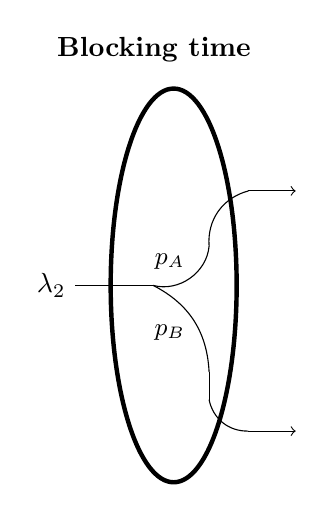
\begin{tikzpicture}
        \draw[ultra thick] (0.75,2) ellipse (0.8cm and 2.5cm);
        \node at (0.5, 5) {\textbf{Blocking time}};
        \draw[-] (0.5, 2) -- ++(-1, 0) node[left] {\(\lambda_2\)};

        % p_A line
        \path (0.49, 2) edge [bend right=50] (1.2, 2.5);
        \path (1.2, 2.5) edge [bend left=40] (1.7, 3.2);
        \draw[->] (1.7, 3.2) -- ++(0.6, 0.);

        % p_B line
        \path (0.49, 2) edge [bend left=30] (1.2, 0.9);
        \draw[-] (1.2, 0.9) -- (1.2, 0.55);
        \path (1.2, 0.55) edge [bend right=40] (1.7, 0.15);
        \draw[->] (1.7, 0.15) -- ++(0.6, 0.);

        \node at (0.7, 2.3) {\small{\( p_A \)}};
        \node at (0.7, 1.4) {\small{\( p_B \)}};
    \end{tikzpicture}
\end{minipage}
\begin{minipage}{.65\textwidth}
    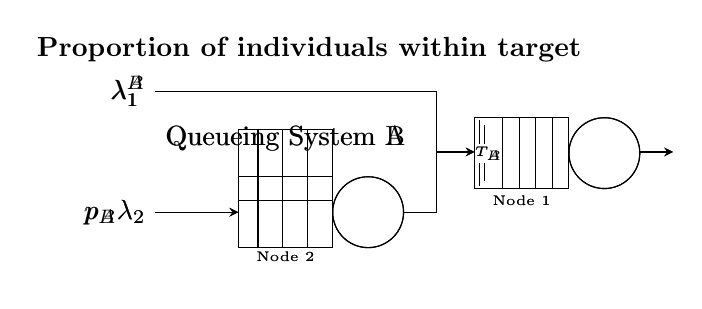
\begin{tikzpicture}[>=stealth, scale=0.6] %arrow type
        % Difference between the two queue diagrams
        
        \tikzmath{
            let \diff = -5cm;
        }
            
        % QUEUEING SYSTEM A
        \node at (1.5cm, 2.7cm) {\textbf{Proportion of individuals within target}};
        \node at (1cm, 0.8cm) {Queueing System A};
            
        % the rectangle with vertical lines (Node 2)
        \draw (0,0) -- ++(2cm,0) -- ++(0,-1.5cm) -- ++(-2cm,0);
        \foreach \i in {1,...,3, 3.8}
        \draw (2cm-\i*15pt,0) -- +(0,-1.5cm);
        \node at (1, -1.7) {\tiny{Node 2}};

        % the circle (Node 2)
        \draw (2.75,-0.75cm) circle [radius=0.75cm];

        % the rectangle with vertical lines (Node 1)
        \draw (5,1.25) -- ++(2cm,0) -- ++(0,-1.5cm) -- ++(-2cm,0);
        \foreach \i in {1,...,4, 5.7}
        \draw (7cm-\i*10pt,1.25) -- +(0,-1.5cm);
        \node at (6, -0.5) {\tiny{Node 1}};

        % The two vertical lines at the start of Node 1
        \draw (7cm-54pt, 1.2cm) -- +(0,-0.5cm);
        \draw (7cm-54pt, 0.3cm) -- +(0,-0.5cm);
        \draw (7cm-51pt, 1.1cm) -- +(0,-0.4cm);
        \draw (7cm-51pt, 0.3cm) -- +(0,-0.4cm);

        % The label between the lines for T
        \node[anchor=north] at (5.3, 0.84) {\tiny{\( T_A \)}};

        % the circle (Node 1)
        \draw (7.75,0.5) circle [radius=0.75cm];

        % the arrows and labels (Node 2+2)
        \draw[->] (8.5,0.525) -- +(20pt,0);
        \node[align=center] at (1cm,-2cm) {};
        \node[align=center] at (6cm,-0.75cm) {};

        % Ambulance lines
        \draw[<-] (0,-0.75) -- +(-50pt,0) node[left] {\( p_A \lambda_2 \)};
        \draw[-] (3.5,-0.75) -- +(20pt,0);
        \draw (4.2, 0.525) -- (4.2, -0.75);

        % Others lines
        \draw (4.2, 1.8) -- +(-169.5pt,0) node[left] {\( \lambda_1^A \)};
        \draw (4.2, 1.8) -- (4.2, 0.525);
        \draw[->] (4.2, 0.525) -- (5, 0.525);


        % QUEUEING SYSTEM B
        \node at (1cm, \diff + 0.8cm) {Queueing System B};

        % the rectangle with vertical rules (Node 2)
        \draw (0, \diff) -- ++(2cm,0) -- ++(0,-1.5cm) -- ++(-2cm,0);
        \foreach \i in {1,...,3, 3.8}
        \draw (2cm-\i*15pt,\diff) -- +(0,-1.5cm);
        \node at (1cm, \diff - 1.7cm) {\tiny{Node 2}};

        % the circle (Node 2)
        \draw (2.75,\diff - 0.75cm) circle [radius=0.75cm];

        % the rectangle with vertical rules (Queue 2)
        \draw (5,\diff + 1.25cm) -- ++(2cm,0) -- ++(0,-1.5cm) -- ++(-2cm,0);
        \foreach \i in {1,...,4, 5.7}
        \draw (7cm-\i*10pt,\diff + 1.25cm) -- +(0,-1.5cm);
        \node at (6, \diff - 0.5cm) {\tiny{Node 1}};

        % The two vertical lines at the start of Queue 2
        \draw (7cm-54pt,\diff + 1.2cm) -- +(0,-0.5cm);
        \draw (7cm-54pt,\diff + 0.3cm) -- +(0,-0.5cm);
        \draw (7cm-51pt,\diff + 1.1cm) -- +(0,-0.4cm);
        \draw (7cm-51pt,\diff + 0.3cm) -- +(0,-0.4cm);

        % The label between the lines for T
        \node[anchor=north] at (5.3, \diff + 0.84cm) {\tiny{\( T_B \)}};

        % the circle (Queue 2)
        \draw (7.75,\diff + 0.5cm) circle [radius=0.75cm];

        % the arrows and labels (Node 2+2)
        \draw[->] (8.5, \diff + 0.525cm) -- +(20pt,0);
        \node[align=center] at (1cm,\diff-2cm) {};
        \node[align=center] at (6cm,\diff-0.75cm) {};

        % Ambulance lines
        \draw[<-] (0, \diff - 0.75cm) -- +(-50pt,0) node[left]
        {\( p_B \lambda_2 \)};
        \draw[-] (3.5, \diff - 0.75cm) -- +(20pt,0);
        \draw (4.2, \diff + 0.525cm) -- (4.2, \diff - 0.75cm);

        % Others lines
        \draw (4.2, \diff + 1.8cm) -- +(-169.5pt,0) node[left]
        {\( \lambda_1^B \)};
        \draw (4.2, \diff + 1.8cm) -- (4.2, \diff + 0.525);
        \draw[->] (4.2, \diff + 0.525cm) -- (5, \diff + 0.525cm);
    \end{tikzpicture}
\end{minipage}

    \caption{A diagrammatic representation of the game theoretic model listing
    the performance measures that correspond to each player's utilities.}
    \label{fig:diagram_of_game_theoretic_model_objectives}
\end{figure}


The payoffs of the players are directly related to the performance measures of
the queueing networks.
More specifically the utilities of the queueing systems focus on the proportion
of individuals whose waiting time and service time falls within a predefined
time target, where this is defined in
Section~\ref{sec:proportion_of_individuals_within_time}.
Similarly the utilities of the distribution service focus on the blocking time
of the queueing systems defined in Section~\ref{sec:blocking_time}.

Consider the queueing system players first.
The objective of either queueing system should be to pick a threshold so that
their own mean waiting time is minimised.

\begin{equation}\label{eq:game_theoretic_alternative_objective_queueing_system_A}
    \arg \min_{T_i} \quad \mathbb{E}[W_i] \quad i \in {A, B}
\end{equation}

The mean waiting time is defined in Section~\ref{sec:waiting_time} as the
average time that an individual spends in node 1.
Although this might seem like a sensible objective at first glance, it is not
necessarily a realistic one.
By using the utility function of
equation~\eqref{eq:game_theoretic_alternative_objective_queueing_system_A}
the queueing systems best response will always be to pick strategy of \(T=1\).
A threshold of \(T=1\) will always result in the lowest mean waiting time
since it will prevent type 2 individuals from entering node 1 as long as there
is at least one individual in node 1.
Depending on the number of available servers this might be true for other values
of \(T\) as well.
For example if there is one available server in node 1, then a threshold of
\(T=1\) will always result in a mean waiting time of zero for type 2
individuals.
That is because type 2 individuals can only enter node 1 if there is nobody
else in node 1, which means that there will always be a free server for type 2
individuals.
Similarly if there are two available servers in node 1, then a threshold of
either \(T=1\) or \(T=2\) will also result in a mean waiting time of zero for
type 2 individuals.

Therefore a more sophisticated objective that doesn't force the queueing systems
to pick the lowest threshold is also considered.
The new objective function is defined as:

\begin{equation}\label{eq:obj_queueing_systems}
    \arg \max_{T_i} \quad 1 - \left( \hat{P} - P(W_i < t) \right)^2
    \qquad i \in {A, B}
\end{equation}

where \(W\) is the waiting time of a potential individual, \(t\) is the time
target and \(\hat{P}\) is the percentage target of individuals that need to be
within that target.
In other words, their aim is to find the threshold that minimises the
difference between the probability \(P(W_i < t)\) and the percentage goal,
or maximise its negation.

The third player, the distribution service, has its own choices to make and
its own goals to satisfy.
The strategy set of the third player is a proportion \(0 \leq p_A \leq 1\)
that corresponds to the proportion of individuals to send to queueing system A
(defined in
equation~\eqref{eq:game_strategy_space_distribution_service_simplified}).
The choice of \(p_A\) and \(p_B\), are based on minimising any potential
blockages that may occur, given the pair of thresholds chosen by the two
queueing systems.
Thus, its objective is to minimise the blocked time of the individuals
(\(B_A\) and \(B_B\)) that they send to queueing systems \(A\) and \(B\).

Apart from the time being blocked, an additional aspect that may affect the
decision of the distribution service is the probability that an individual
becomes lost to a queueing system.
A type 2 individual can become lost to a queueing system if they arrive in a
queueing system and node 2 is at its maximum capacity \(M\).
Therefore, the probability that an individual is lost to queueing system \(i\)
is given by \(L_i\) where \(i \in \{A, B\}\):

\begin{equation}\label{eq:probability_lost}
    L_i = \sum_{\substack{(u, v) \in S \\ u = M}} \pi_{(u, v)}
\end{equation}

where \(S\) is the set of all states in queueing system \(i\), \(M\) is the
maximum capacity of node 2 and \(\pi_{(u, v)}\) is the probability of being in
state \((u, v)\) (as defined in Section~\ref{sec:queueing_section}).

For each queueing system, there is a penalty of sending a proportion of \(p_i\)
individuals to that queueing system.
That penalty is given by:

\begin{equation}\label{eq:obj_distributor_penalty}
    \alpha L_i(p_i) + (1 - \alpha) B_i(p_i), \quad i \in {A, B}
\end{equation}

Equation~\eqref{eq:obj_distributor_penalty} can be used to capture a mixture
between the two objectives \(L_i\) and \(B_i\) where \(i \in \{A, B\}\).
Here, \(\alpha\) represents the ``weight'' of each
objective~\cite{gunantara2018review},
where a high \(\alpha\) indicates a higher weight on the proportion of lost
individuals and a smaller \(\alpha\) a higher weight on the time blocked.
In fact, the best response of the distribution service can be found by equating
the penalty of sending \(p_A\) individuals to queueing system \(A\) and the
penalty
of sending \(p_B\) individuals to queueing system \(B\) (where \(p_B = 1-p_A\)).

\begin{equation}\label{eq:obj_distributor_1}
    \alpha L_A(p_A) + (1 - \alpha) B_A(p_A) =
    \alpha L_B(p_B) + (1 - \alpha) B_B(p_B)
\end{equation}

There are some cases where the best response of the distribution service is
to distribute all individuals to one of the two queueing systems.
For example, if queueing system \(A\) has a low threshold and queueing system
\(B\)
has a high threshold, then the distribution service's best response may be to
send all individuals to queueing system \(B\).
Thus equation~\eqref{eq:obj_distributor_1} can be modified to be:

\begin{equation*}
    O(p_A; T_A, T_B) = \alpha L_A(p_A) + (1 - \alpha) B_A(p_A) -
    \alpha L_B(1 - p_A) - (1 - \alpha)B_B(1 - p_A)
\end{equation*}
\begin{equation}\label{eq:obj_distributor_2}
    \arg \min_{p_A} |O(p_A; T_A, T_B)|
\end{equation}


The choice of \(p_A\) and \(p_B\) rely solely on
equation~\eqref{eq:obj_distributor_2}.
Note that the current system is modelled using unobservable queues which is not
necessarily an unrealistic approach~\cite{unobservablequeue}.
Another approach would be to allow the distribution service to observe the
state of each queueing system before sending each individual to either of them
and making a decision based on that state.
There are several other factors that can affect the routing of the
individuals that are outside the scope of this thesis.
For example the distance from the distribution service to each queueing system
or even the priority level of each individual may be a significant factor that
affects the distribution service's decision.



\subsection{Imperfect information extensive form game}

The game can be modelled as an imperfect information extensive form game as
described in Section~\ref{sec:game_imperfect_information}.
The strategies and payoffs of all players can be put together to form the
following game tree:

\begin{figure}[H]
    \centering
    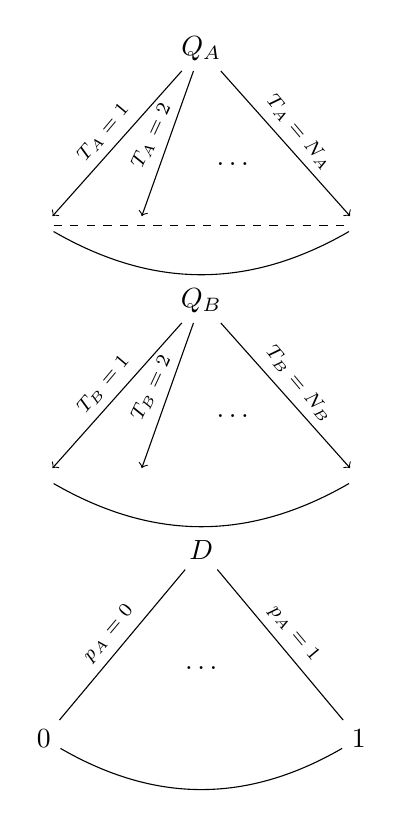
\begin{tikzpicture}[-, node distance = 2cm, scale=0.8]
    \node[anchor=north](QA){\(Q_A\)};
    \node[anchor=north](QA_d1) at (-2.5, -3) {};
    \node[anchor=north](QA_d2) at (-1, -3) {};
    \node[anchor=north](QA_d3) at (0.5, -2) {\(\dots\)};
    \node[anchor=north](QA_d4) at (2.5, -3) {};

    \path[->] (QA) edge node [above, rotate=50] {\scriptsize{\(T_A=1\)}}(QA_d1);
    \path[->] (QA) edge node [above, rotate=65] {\scriptsize{\(T_A=2\)}}(QA_d2);
    \path[<-] (QA_d4) edge node [above, rotate=310] {\scriptsize{\(T_A = N_A\)}}(QA);

    \path (QA_d1) [dashed] edge node {}(QA_d4);
    \path (QA_d1) [bend right] edge node {}(QA_d4);

    \node[anchor=north](QB) at (0, -4) {\(Q_B\)};
    \node[anchor=north](QB_d1) at (-2.5, -7) {};
    \node[anchor=north](QB_d2) at (-1, -7) {};
    \node[anchor=north](QB_d3) at (0.5, -6) {\(\dots\)};
    \node[anchor=north](QB_d4) at (2.5, -7) {};

    \path[->] (QB) edge node [above, rotate=50] {\scriptsize{\(T_B=1\)}}(QB_d1);
    \path[->] (QB) edge node [above, rotate=65] {\scriptsize{\(T_B=2\)}}(QB_d2);
    \path[<-] (QB_d4) edge node [above, rotate=310] {\scriptsize{\(T_B = N_B\)}}(QB);

    \path (QB_d1) [bend right] edge node {}(QB_d4);

    \node[anchor=north] (D) at (0, -8) {\(D\)};
    \node[anchor=north](D_d1) at (-2.5, -11) {0};
    \node[anchor=north](D_dots) at (0, -10) {\(\dots\)};
    \node[anchor=north](D_d2) at (2.5, -11) {1};

    \path[-] (D) edge node [above, rotate=50] {\scriptsize{\(p_A=0\)}}(D_d1);
    \path[-] (D_d2) edge node [above, rotate=310] {\scriptsize{\(p_A=1\)}}(D);

    \path (D_d1) [bend right] edge node {}(D_d2);

\end{tikzpicture}

    \caption{Imperfect information extensive form game between the distribution
    service and the 2 queueing systems}
    \label{fig:imperfect_info_game}
\end{figure}

The game tree is a representation of all possible sequences of decisions that
can be made by the players.
Initially, queueing system \(A\) chooses which threshold \(T_A\) to play out of
\(N_A\) possible choices.
Then, queueing system \(B\) chooses its own threshold \(Q_B\) without knowing
the threshold chosen by queueing system \(A\).
Note here that it doesn't matter which queueing system chooses its threshold
first since the other queueing system will always choose its threshold
independently of the first queueing system's choice.
Afterwards, the distribution service chooses the proportion of individuals to
send to queueing system \(A\), from the continuous strategy space of
\(0 \leq p_A \leq 1\).
The distribution service has all the information about the state that the game
is at when it's choosing the value of \(p_A\).
Thus, the distribution service's choice of \(p_A\) is based on the thresholds
chosen by the queueing systems.
The payoffs for all players are then calculated.

\section{Methodology}

A big part of the methodology that is used to solve the game requires the use of
backwards induction.
Backwards induction is a method that is used to solve a game by starting at the
terminal nodes and working backwards to the root node~\cite{watson2002strategy}.
The terminal nodes from Figure~\ref{fig:imperfect_info_game} are the nodes that
are connected to the choice of the distribution service.
In essence, by working backwards from the choice of the distribution service
and then to the choices of the queueing systems, which happen simultaneously,
the game can be solved.
Furthermore, by finding the distribution's service response for all possible
pairs of strategies that the two queueing systems can choose from, the game can
be reduced to a two-player Normal form game.


\subsection{Distribution service and Brent's algorithm}
\label{sec:best_response_distribution_service}

Form the distribution service's perspective all information is known and can be
used to find the best possible strategy to maximise their payoff.
In fact, having the two strategy choices of the two queueing systems the
distribution service can find the optimal strategy that satisfies
equation~(\ref{eq:obj_distributor_2}).
Consider the pair of strategies \((T_A^*, T_B^*)\) that correspond to a possible
strategy choice of queueing system \(A\) and queueing system \(B\).
The distribution service can then find the best strategy by solving
equation~(\ref{eq:obj_distributor_2}) for \(T_A = T_A^*\) and \(T_B = T_B^*\).
The particular numerical algorithm used for this is Brent's
algorithm~\cite{brent_method}.

Brent's algorithm is a root-finding algorithm which combines the bisection
method~\cite{corliss1977root}, the secant method~\cite{secantmethod} and
inverse quadratic interpolation~\cite{epperson2021introduction}.
The algorithm is used to find the root \(x^*\) of a function \(f(x)\) from
within the interval \([a, b]\) such that \(f(a) < f(x^*) < f(b)\).
One of the requirements for Brent's algorithm is \(f(a)f(b) < 0\).
In other words the function must change sign within the interval \([a, b]\).

Consider equation (\ref{eq:obj_distributor_2}).
Under the assumption that \(O(p_A; T_A, T_B)\) is either non-increasing or
non-decreasing in \(p_A\), the root can be found by using Brent's algorithm
for \(p_A \in [0, 1]\).

\begin{equation*}
    O(p_A; T_A, T_B) = \alpha L_A(p_A) + (1 - \alpha) B_A(p_A) -
    \alpha L_B(1 - p_A) - (1 - \alpha)B_B(1 - p_A)
\end{equation*}

For this particular scenario, the function \(f(p_A)\) needs to have a different
sign for \(f(p_A = 0)\) and \(f(p_A = 1)\) so that \(f(a)f(b) < 0\) is
satisfied.
In the case \(f(a)f(b) \geq 0\), Brent's algorithm cannot be used.
Instead, the value of \(p_A\) becomes:

\begin{equation}\label{eq:obj_distributor_no_brent_method}
    p_A = \begin{cases}
        1 & \text{if } f(0) < 0 \text{ and } f(1) < 0 \\
        0 & \text{if } f(0) > 0 \text{ and } f(1) > 0
    \end{cases}
\end{equation}

The first case of equation~(\ref{eq:obj_distributor_no_brent_method})
corresponds to the event where both \(f(0)\) and \(f(1)\) are negative.
Therefore, for all values of \(p_A \in [0, 1]\) the objective function is
negative, which means that:

\[
    \alpha L_A(p_A) + (1 - \alpha) B_A(p_A) <
    \alpha L_B(p_B) - (1 - \alpha) B_B(p_B), \quad \text{for all } p_A \in [0,1]
\]

Thus, the distribution service's best response would be to send all individuals
to queueing system \(A\) (\(p_A=1, p_B=0\)).
Similarly, the second case of
equation~(\ref{eq:obj_distributor_no_brent_method}) corresponds to the event
where for all values of \(p_A \in [0, 1]\) the objective function is
positive, which means that:

\[
    \alpha L_A(p_A) + (1 - \alpha) B_A(p_A) >
    \alpha L_B(p_B) - (1 - \alpha) B_B(p_B), \quad \text{for all } p_A \in [0,1]
\]

Equivalently, this indicates that the distribution service's best response
would be to send all individuals to queueing system \(B\) (\(p_A=0, p_B=1\)).
Therefore, the methodology that is used to find the best \(p_A\) that satisfies
equation~(\ref{eq:obj_distributor_2}) can by calculated in the following way:

\begin{equation}\label{eq:obj_distributor_implementation}
    p_A = \begin{cases}
        1, & \text{if } O(0) < 0 \text{ and } O(1) < 0 \\
        0, & \text{if } O(0) > 0 \text{ and } O(1) > 0 \\
        \text{Use Brent's algorithm}, & \text{if } O(0)O(1) < 0
    \end{cases}
\end{equation}

where \(O(p_A)\) is the objective function of the distribution service described
in equation~(\ref{eq:obj_distributor_2}).

\subsubsection{Examples}\label{sec:brent_method_example}
Consider a distribution service whose arrival rate of type 2 individuals is
\(\lambda_2 = 4\) and the `weight' is \(\alpha = 0.2\).
Additionally, let queueing system \(A\) and queueing system \(B\) have the
following parameters:

\begin{multicols}{2}
    \begin{itemize}
        \item \(\lambda_1^A = 2\)
        \item \(\mu^A = 3\)
        \item \(C^A = 3\)
        \item \(T^A = 8\)
        \item \(N^A = 15\)
        \item \(M^A = 10\)
        \item \(\lambda_1^B = 1\)
        \item \(\mu^B = 1\)
        \item \(C^B = 3\)
        \item \(T^B = 10\)
        \item \(N^B = 10\)
        \item \(M^B = 5\)
    \end{itemize}
\end{multicols}

The distribution service's best response for this particular example can be
found at the intersection of the two decision values of the two queueing
systems over \(p_A\).
Figure~\ref{fig:brent_method_example} illustrates the distribution service's
best response for this particular example.

\begin{figure}[H]
    \centering
    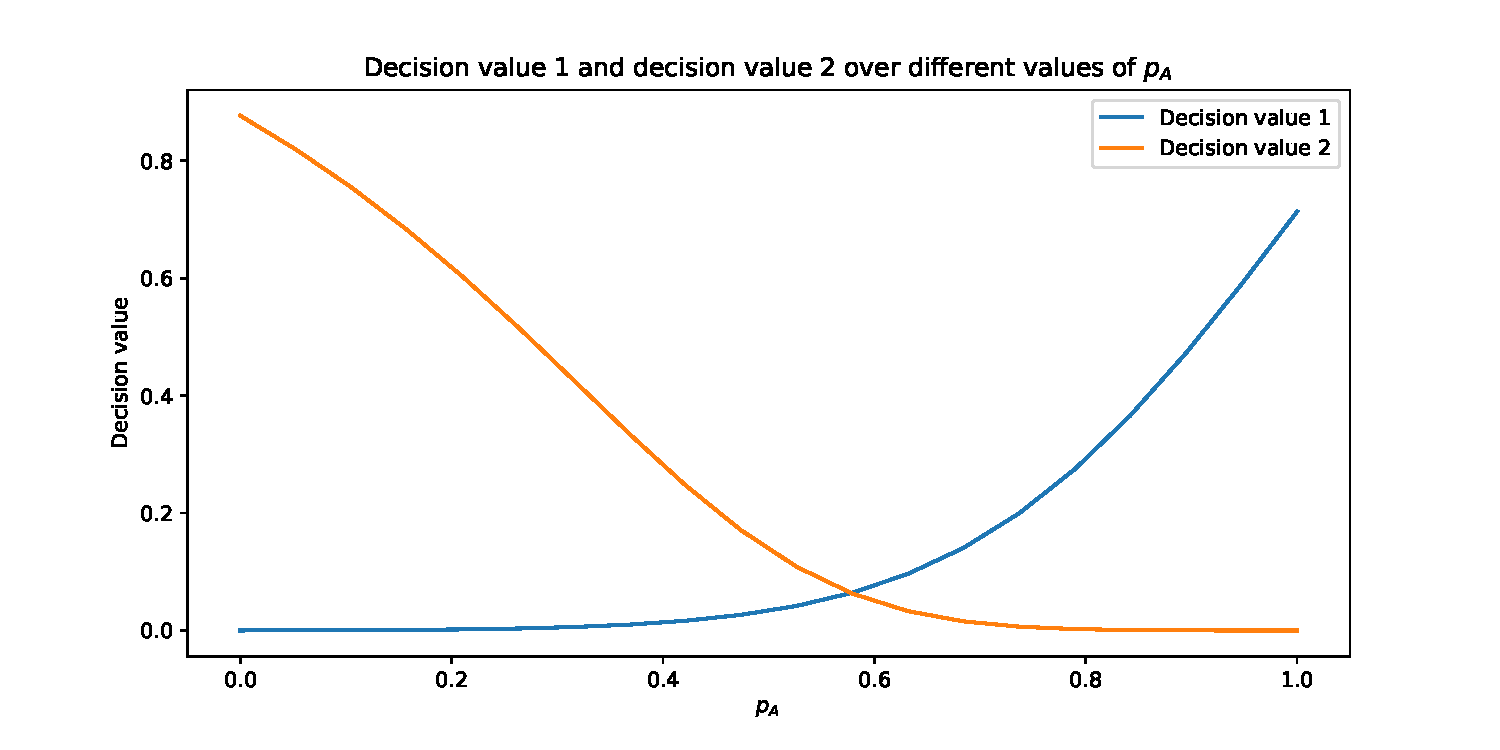
\includegraphics[width=\textwidth]{chapters/04_game_theoretic_model/img/brents_method/brent_method_example.pdf}
    \caption{Decision values for queueing system \(A\) and queueing system \(B\)}
    \label{fig:brent_method_example}
\end{figure}

In order to apply Brent's algorithm to the current example the differences
between the two decision values need to be calculated.
Figure~\ref{fig:brent_method_diffs} shows that the value of \(p_A\) that the
distribution service should pick is where the function crosses the \(x\)-axis.

\begin{figure}[H]
    \centering
    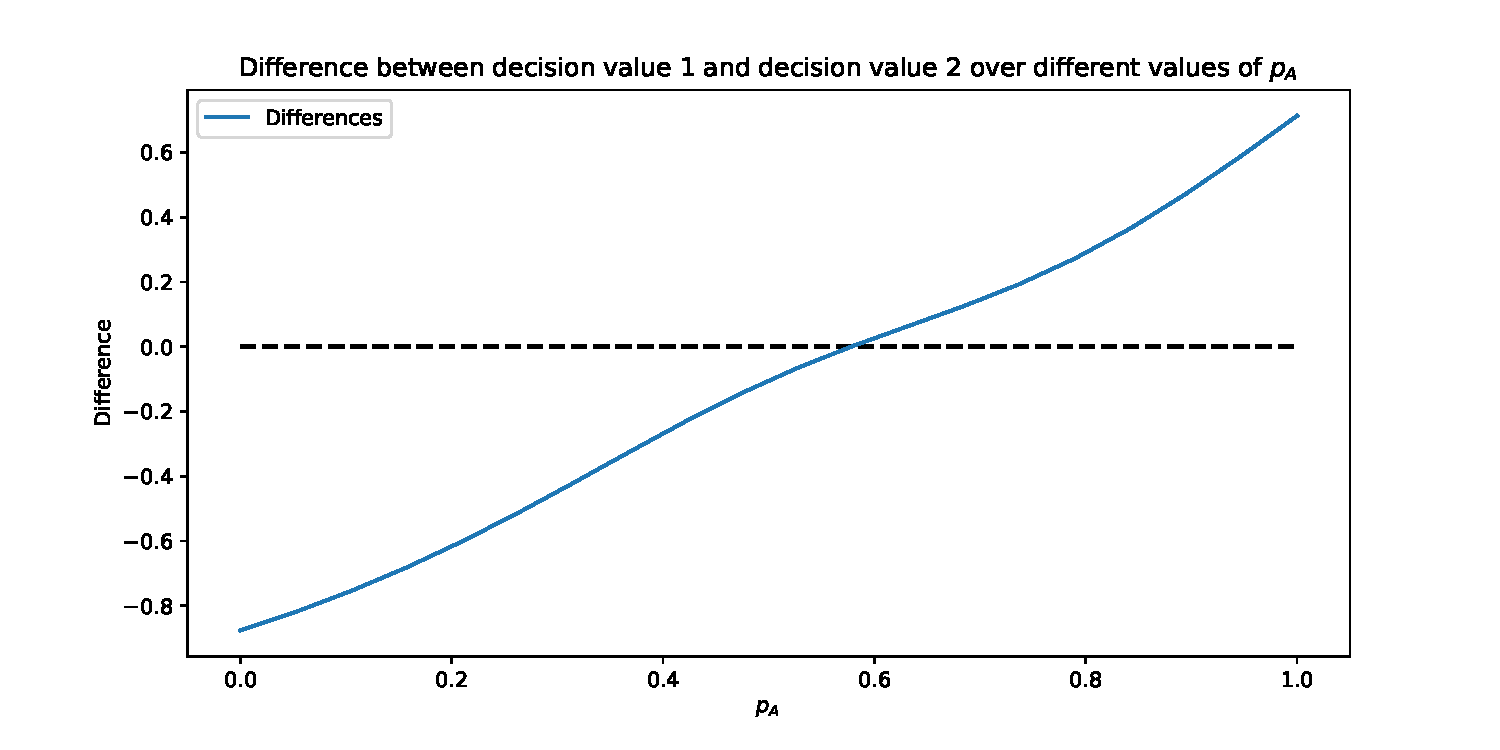
\includegraphics[width=\textwidth]{chapters/04_game_theoretic_model/img/brents_method/brent_method_diffs.pdf}
    \caption{Brent's algorithm on the differences}
    \label{fig:brent_method_diffs}
\end{figure}

In fact, the value of \(p_A\) that the distribution service should pick, for
this particular example, is \(p_A = 0.58\).
That is the point at which the line of the difference between the two decision
values crosses the \(x\)-axis.

Consider now the same parameters as in the previous example, for different
values of the service rate of queueing system \(A\), \(\mu^A =
\{1,1.5,2,2.5,3\}\).

\begin{figure}[H]
    \centering
    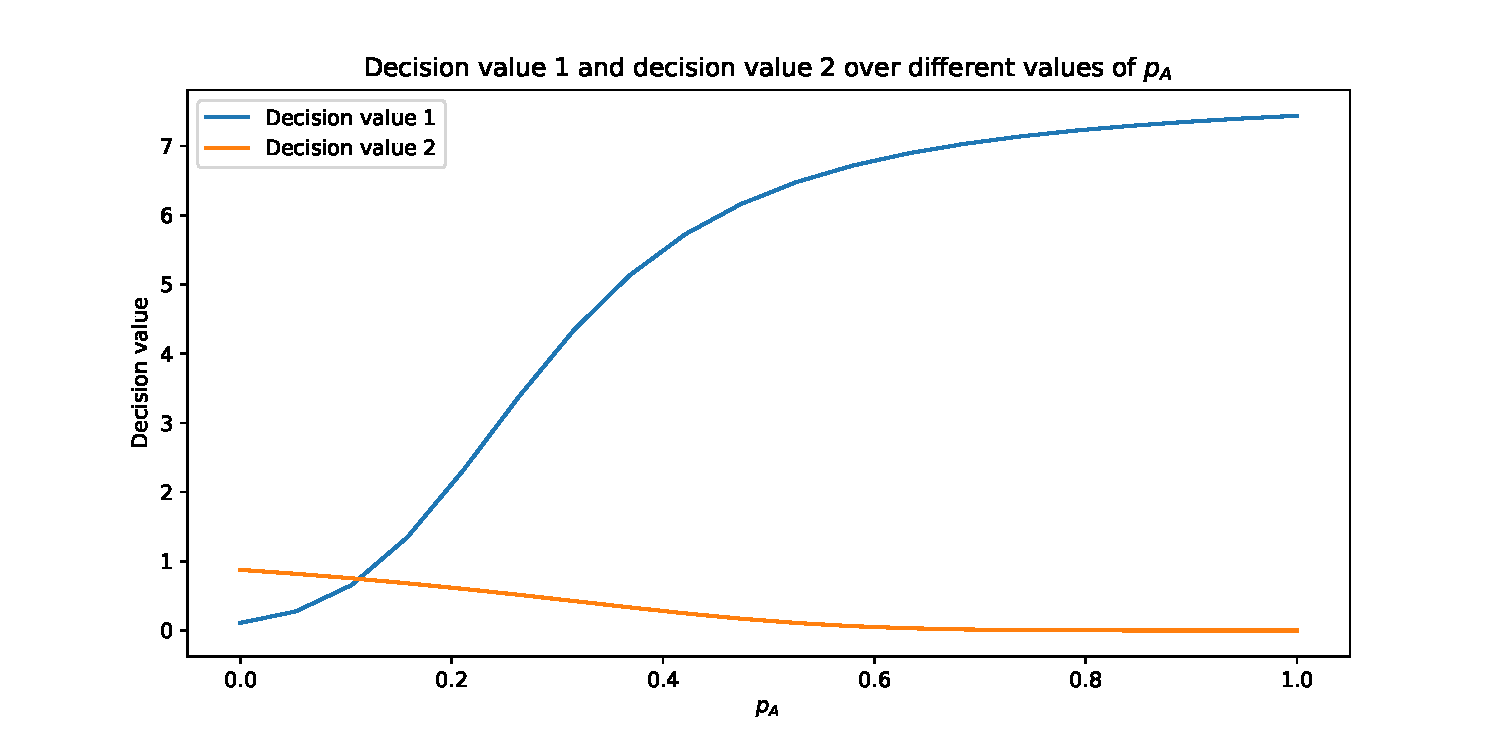
\includegraphics[width=\textwidth]{chapters/04_game_theoretic_model/img/brents_method/brent_method_example_mu_A_1.0.pdf}
    \caption{\(\mu^A = 1\)}
    \label{fig:brent_method_example_mu_A_1}
\end{figure}

\begin{figure}[H]
    \centering
    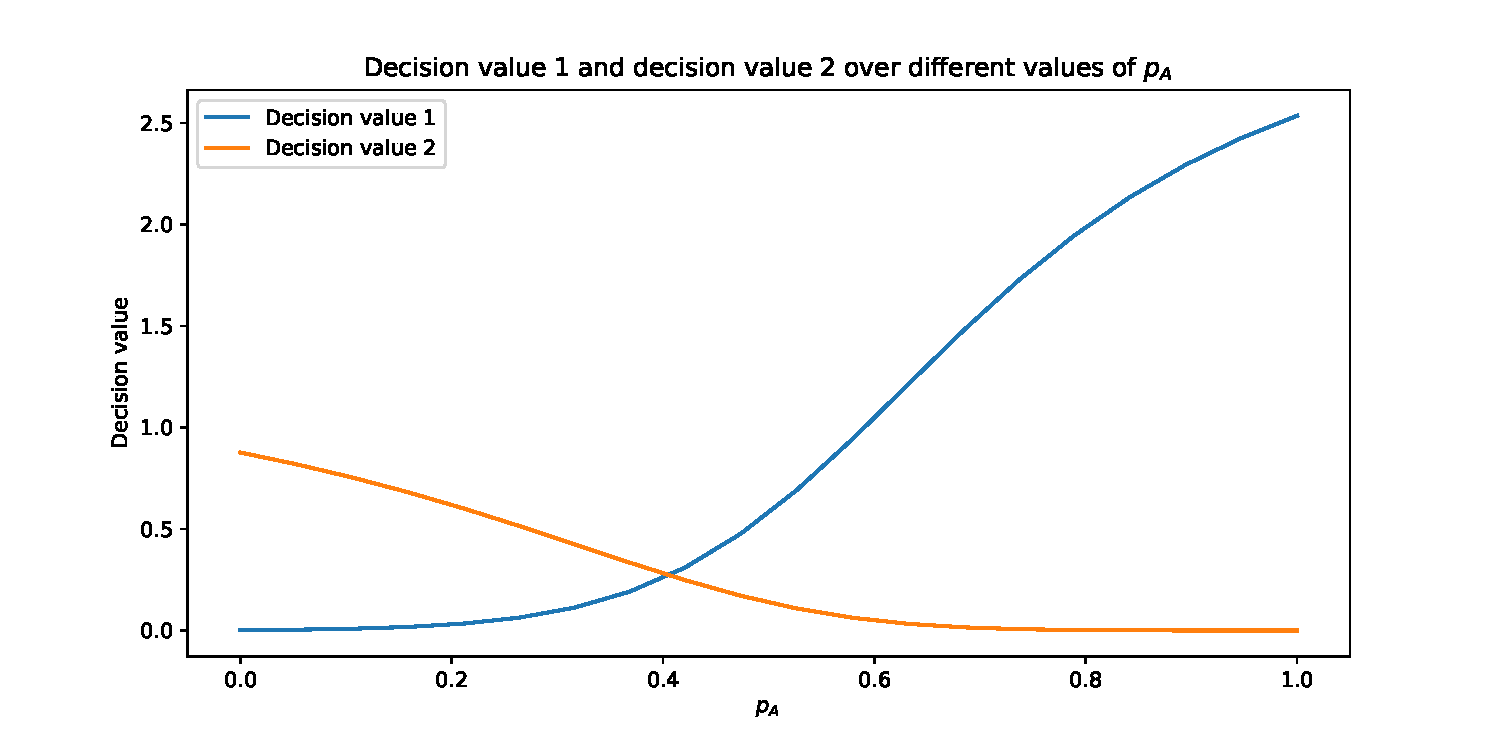
\includegraphics[width=\textwidth]{chapters/04_game_theoretic_model/img/brents_method/brent_method_example_mu_A_1.5.pdf}
    \caption{\(\mu^A = 1.5\)}
    \label{fig:brent_method_example_mu_A_2}
\end{figure}

\begin{figure}[H]
    \centering
    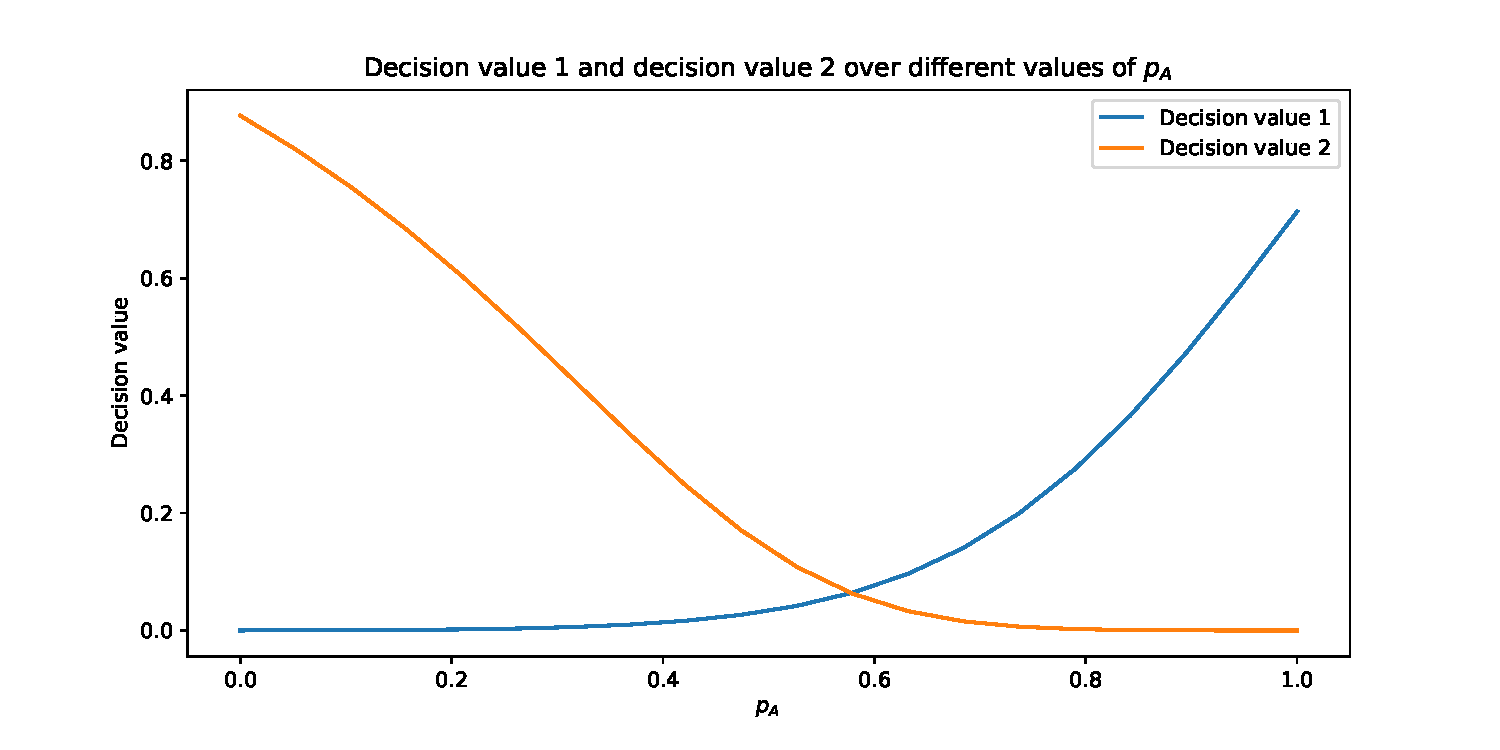
\includegraphics[width=\textwidth]{chapters/04_game_theoretic_model/img/brents_method/brent_method_example_mu_A_2.0.pdf}
    \caption{\(\mu^A = 2\)}
    \label{fig:brent_method_example_mu_A_3}
\end{figure}

\begin{figure}[H]
    \centering
    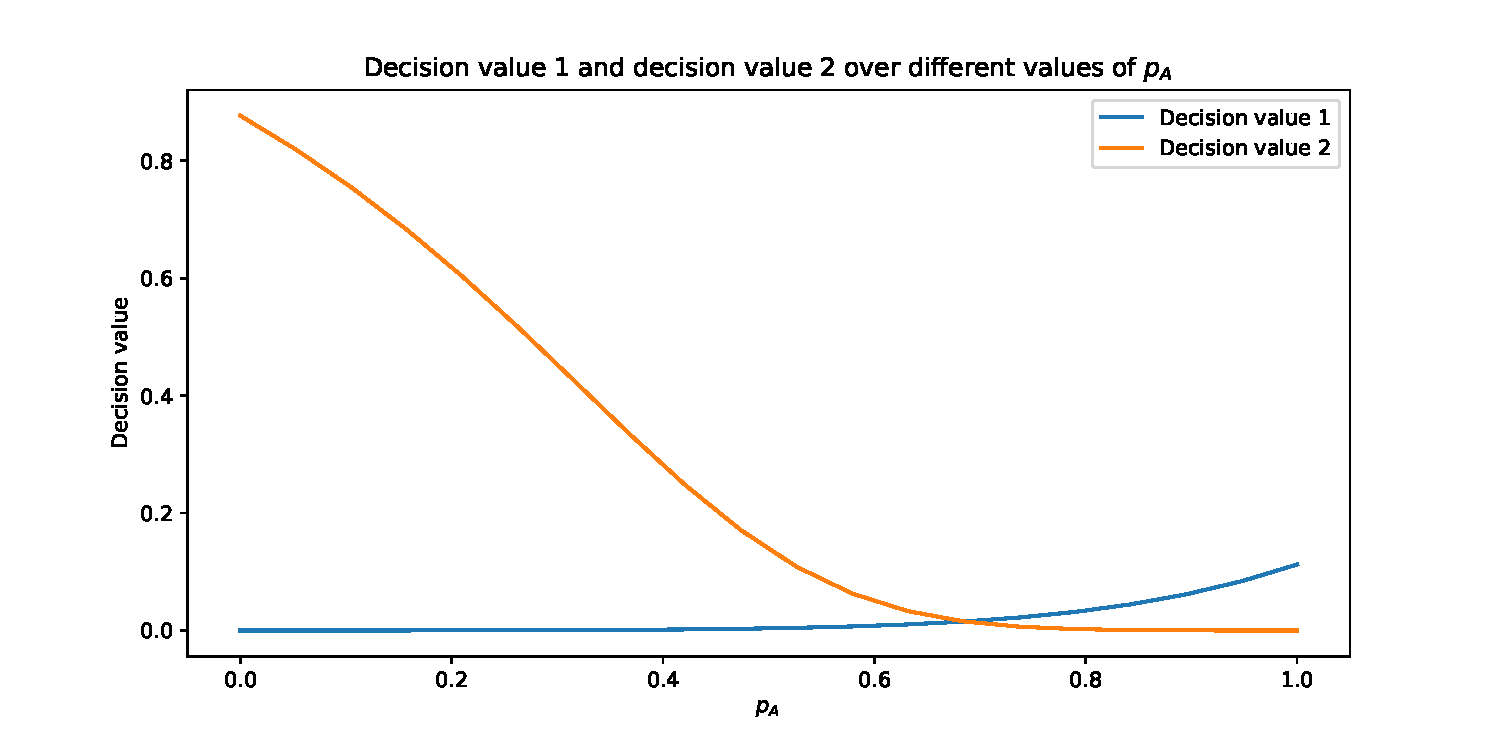
\includegraphics[width=\textwidth]{chapters/04_game_theoretic_model/img/brents_method/brent_method_example_mu_A_2.5.pdf}
    \caption{\(\mu^A = 2.5\)}
    \label{fig:brent_method_example_mu_A_4}
\end{figure}

\begin{figure}[H]
    \centering
    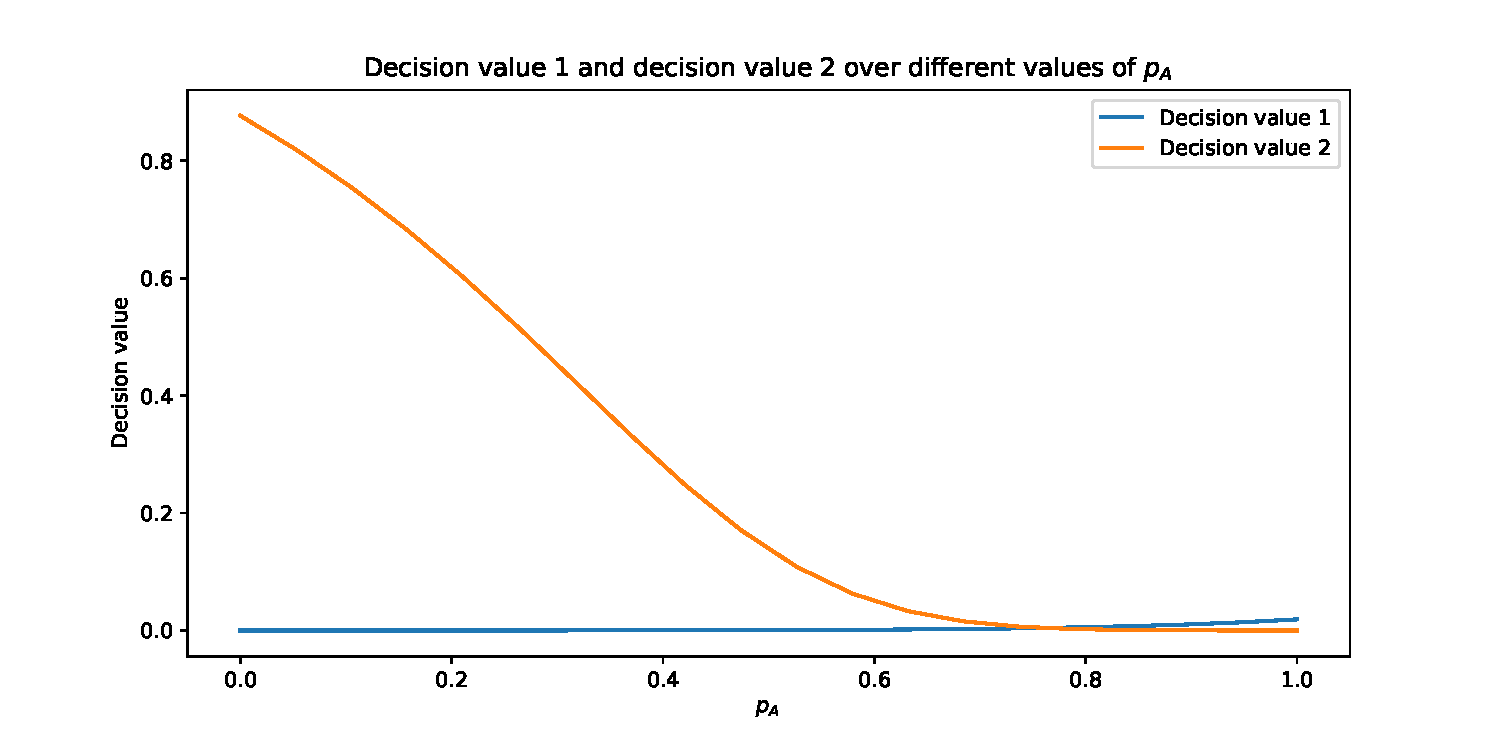
\includegraphics[width=\textwidth]{chapters/04_game_theoretic_model/img/brents_method/brent_method_example_mu_A_3.0.pdf}
    \caption{\(\mu^A = 3\)}
    \label{fig:brent_method_example_mu_A_5}
\end{figure}

It can be seen from Figures~\ref{fig:brent_method_example_mu_A_1} -
\ref{fig:brent_method_example_mu_A_5} that as the service rate of queueing
system \(A\) increases, the intersection point of the two decision values moves
from \(p_A=0\) towards \(p_A=1\).

In addition consider a different example with the same parameters as before
but by increasing the threshold of queueing system \(A\) from \(T^A = 8\) to
\(T^A = 10\) and decreasing the threshold of queueing system \(B\) from
\(T^B = 10\) to \(T^B = 2\).
Figure~\ref{fig:brent_method_special_case} shows the decision values that
correspond to the two queueing systems of the new example.

\begin{figure}[H]
    \centering
    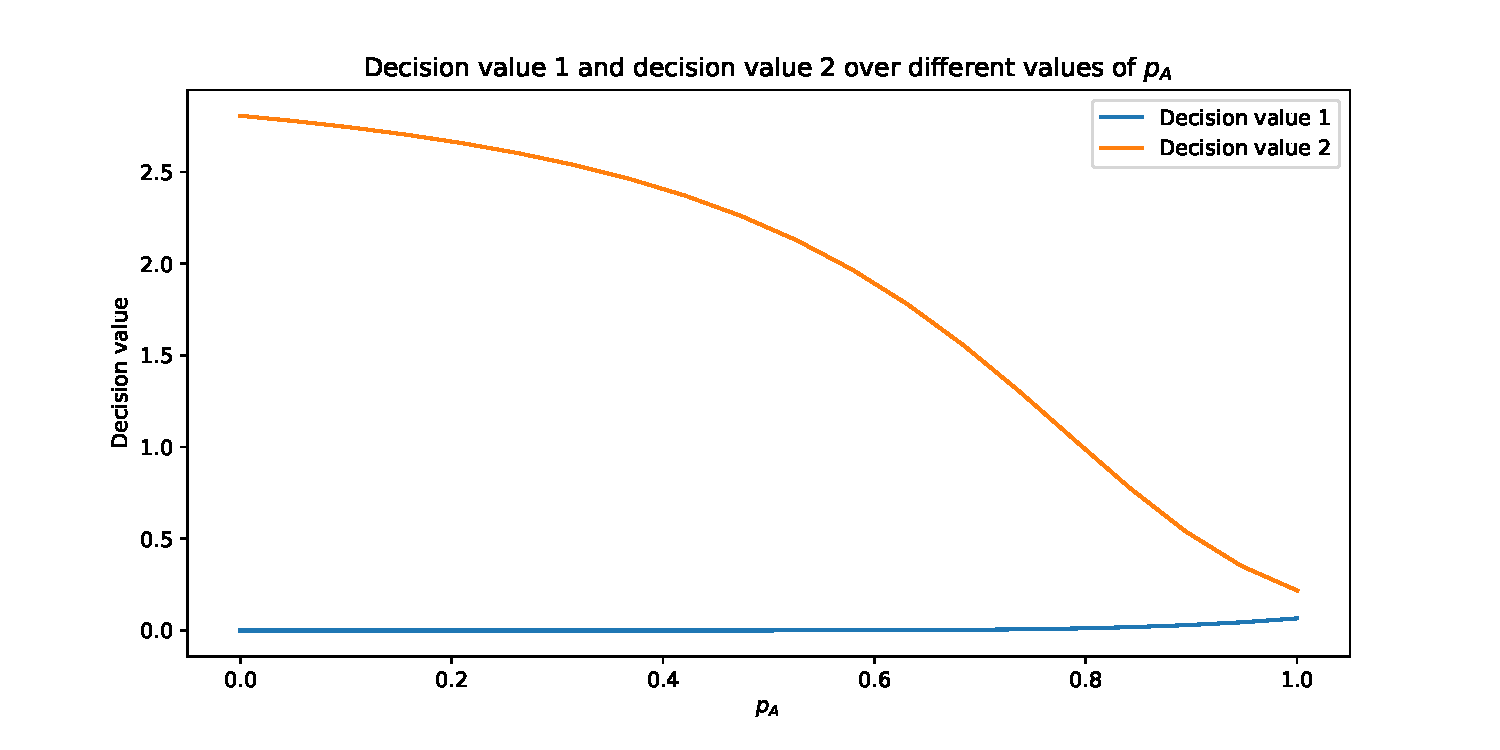
\includegraphics[width=\textwidth]{chapters/04_game_theoretic_model/img/brents_method/brent_method_special_case.pdf}
    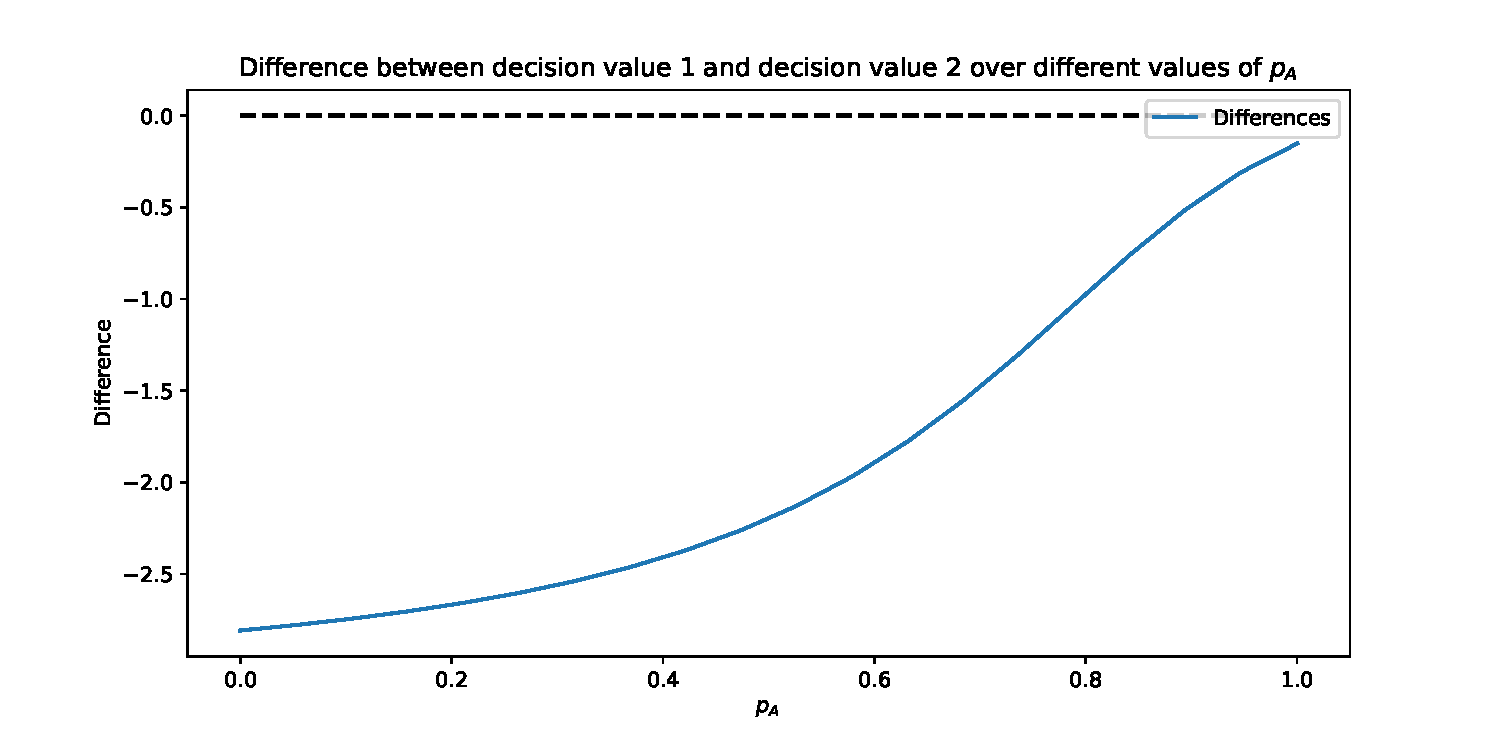
\includegraphics[width=\textwidth]{chapters/04_game_theoretic_model/img/brents_method/brent_method_special_case_diffs.pdf}
    \caption{Decision values for queueing system \(A\) and queueing system \(B\)}
    \label{fig:brent_method_special_case}
\end{figure}

It can be observed that for all values of \(p_A\) the decision value of queueing
system \(A\) is less than the decision value of queueing system \(B\).
Since the differences of them don't pass through the x-axis within the interval
\([0,1]\), Brent's algorithm cannot be used since \(f(0)f(1) < 0\).
Therefore, using equation~(\ref{eq:obj_distributor_implementation}) the
distribution service's best response should be \(p_A = 1\).

\subsubsection{Implementation}

The first part of the implementation of the distribution service's best
response is to calculate the difference between the decision values of the two
queueing systems.
Function \lstinline[style=pystyle]{get_mean_blocking_difference_using_markov}
is the python implementation of the first part of
equation~(\ref{eq:obj_distributor_2}).

\begin{lstlisting}[style=pystyle]
>>> import ambulance_game as abg
>>> def get_mean_blocking_difference_using_markov(
...     prop_1,
...     lambda_2,
...     lambda_1_1,
...     lambda_1_2,
...     mu_1,
...     mu_2,
...     num_of_servers_1,
...     num_of_servers_2,
...     threshold_1,
...     threshold_2,
...     system_capacity_1,
...     system_capacity_2,
...     buffer_capacity_1,
...     buffer_capacity_2,
...     alpha=0,
... ):
...     """
...     Get a weighted mean blocking difference between two systems. This
...     function is to be used as a routing function to find the point at
...     which it is set to 0. This function calculates:
...         - a*(1 - P(A_1)) + (1 - a)*B_1
...         - a*(1 - P(A_2)) + (1 - a)*B_2
...     and returns their difference.
...     Parameters
...     ----------
...     prop_1 : float
...         The proportion of class 2 individuals to distribute to the first
...         system
...     lambda_2 : float
...         The overall arrival rate of class 2 individuals for both systems
...     lambda_1_1 : float
...         The arrival rate of class 1 individuals in the first system
...     lambda_1_2 : float
...         The arrival rate of class 1 individuals in the second system
...     mu_1 : float
...     mu_2 : float
...     num_of_servers_1 : int
...     num_of_servers_2 : int
...     threshold_1 : int
...     threshold_2 : int
...     system_capacity_1 : int
...     system_capacity_2 : int
...     buffer_capacity_1 : int
...     buffer_capacity_2 : int
...     Returns
...     -------
...     float
...         The weighted mean difference between the decision values of the
...         two systems
...     """
...     lambda_2_1 = prop_1 * lambda_2
...     lambda_2_2 = (1 - prop_1) * lambda_2
...
...     mean_blocking_time_1 = abg.markov.get_mean_blocking_time_using_markov_state_probabilities(
...         lambda_2=lambda_2_1,
...         lambda_1=lambda_1_1,
...         mu=mu_1,
...         num_of_servers=num_of_servers_1,
...         threshold=threshold_1,
...         system_capacity=system_capacity_1,
...         buffer_capacity=buffer_capacity_1,
...     )
...     mean_blocking_time_2 = abg.markov.get_mean_blocking_time_using_markov_state_probabilities(
...         lambda_2=lambda_2_2,
...         lambda_1=lambda_1_2,
...         mu=mu_2,
...         num_of_servers=num_of_servers_2,
...         threshold=threshold_2,
...         system_capacity=system_capacity_2,
...         buffer_capacity=buffer_capacity_2,
...     )
...     prob_accept_1 = abg.markov.get_accepting_proportion_of_class_2_individuals(
...         lambda_1=lambda_1_1,
...         lambda_2=lambda_2_1,
...         mu=mu_1,
...         num_of_servers=num_of_servers_1,
...         threshold=threshold_1,
...         system_capacity=system_capacity_1,
...         buffer_capacity=buffer_capacity_1,
...     )
...     prob_accept_2 = abg.markov.get_accepting_proportion_of_class_2_individuals(
...         lambda_1=lambda_1_2,
...         lambda_2=lambda_2_2,
...         mu=mu_2,
...         num_of_servers=num_of_servers_2,
...         threshold=threshold_2,
...         system_capacity=system_capacity_2,
...         buffer_capacity=buffer_capacity_2,
...     )
...
...     decision_value_1 = (
...         alpha * (1 - prob_accept_1) + (1 - alpha) * mean_blocking_time_1
...     )
...     decision_value_2 = (
...         alpha * (1 - prob_accept_2) + (1 - alpha) * mean_blocking_time_2
...     )
...     return decision_value_1 - decision_value_2

\end{lstlisting}

Using the same example as in section~\ref{sec:brent_method_example} the
differences between the two decision values can be calculated using the next
code snippet.
Note, that the outcome of the function corresponds to the point of the line in
Figure~\ref{fig:brent_method_diffs} where \(p_A = 0.5\).

\begin{lstlisting}[style=pystyle]
>>> import numpy as np
>>>
>>> lambda_1_A = 2
>>> mu_A = 2
>>> num_of_servers_A = 3
>>> threshold_A = 8
>>> system_capacity_A = 15
>>> buffer_capacity_A = 10
>>> lambda_1_B = 1
>>> mu_B = 1
>>> num_of_servers_B = 3
>>> threshold_B = 10
>>> system_capacity_B = 10
>>> buffer_capacity_B = 5
>>>
>>> lambda_2 = 4
>>> alpha = 0.2
>>> p_A = 0.5
>>>
>>> np.round(get_mean_blocking_difference_using_markov(
...     prop_1=p_A,
...     lambda_2=lambda_2,
...     lambda_1_1=lambda_1_A,
...     lambda_1_2=lambda_1_B,
...     mu_1=mu_A,
...     mu_2=mu_B,
...     num_of_servers_1=num_of_servers_A,
...     num_of_servers_2=num_of_servers_B,
...     threshold_1=threshold_A,
...     threshold_2=threshold_B,
...     system_capacity_1=system_capacity_A,
...     system_capacity_2=system_capacity_B,
...     buffer_capacity_1=buffer_capacity_A,
...     buffer_capacity_2=buffer_capacity_B,
...     alpha=alpha,
... ), 8)
-0.10424302

\end{lstlisting}

In addition function
\lstinline[style=pystyle]{calculate_class_2_individuals_best_response} uses
an implementation of Brent's algorithm, implemented by the
\lstinline[style=pystyle]{scipy} library, to find the point at which the
difference between the two decision values is set to 0.

\begin{lstlisting}[style=pystyle]
>>> import scipy.optimize
>>> def calculate_class_2_individuals_best_response(
...     lambda_2,
...     lambda_1_1,
...     lambda_1_2,
...     mu_1,
...     mu_2,
...     num_of_servers_1,
...     num_of_servers_2,
...     threshold_1,
...     threshold_2,
...     system_capacity_1,
...     system_capacity_2,
...     buffer_capacity_1,
...     buffer_capacity_2,
...     lower_bound=0.01,
...     upper_bound=0.99,
...     alpha=0,
...     xtol=1e-04,
...     rtol=8.9e-16,
... ):
...     """
...     Obtains the optimal distribution of class 2 individuals such that the
...     blocking times in the two systems are identical and thus minimised.
...     The brentq function is used which is an algorithm created to find the
...     root of a function that combines root bracketing, bisection, and
...     inverse quadratic interpolation. In this specific example the root to
...     be found is the difference between the blocking times of two systems.
...     In essence the brentq algorithm attempts to find the value of prop_1
...     where the difference is zero.
...
...     Parameters
...     ----------
...     lower_bound : float, optional
...         The lower bound of p_1, by default 0.01
...     upper_bound : float, optional
...         The upper bound of p_1, by default 0.99
...     routing_function : function, optional
...         The function to find the root of
...     Returns
...     -------
...     float
...         The value of p_1 such that routing_function = 0
...     """
...
...     routing_function = get_mean_blocking_difference_using_markov
...     check_1 = routing_function(
...         prop_1=lower_bound,
...         lambda_2=lambda_2,
...         lambda_1_1=lambda_1_1,
...         lambda_1_2=lambda_1_2,
...         mu_1=mu_1,
...         mu_2=mu_2,
...         num_of_servers_1=num_of_servers_1,
...         num_of_servers_2=num_of_servers_2,
...         threshold_1=threshold_1,
...         threshold_2=threshold_2,
...         system_capacity_1=system_capacity_1,
...         system_capacity_2=system_capacity_2,
...         buffer_capacity_1=buffer_capacity_1,
...         buffer_capacity_2=buffer_capacity_2,
...         alpha=alpha,
...     )
...     check_2 = routing_function(
...         prop_1=upper_bound,
...         lambda_2=lambda_2,
...         lambda_1_1=lambda_1_1,
...         lambda_1_2=lambda_1_2,
...         mu_1=mu_1,
...         mu_2=mu_2,
...         num_of_servers_1=num_of_servers_1,
...         num_of_servers_2=num_of_servers_2,
...         threshold_1=threshold_1,
...         threshold_2=threshold_2,
...         system_capacity_1=system_capacity_1,
...         system_capacity_2=system_capacity_2,
...         buffer_capacity_1=buffer_capacity_1,
...         buffer_capacity_2=buffer_capacity_2,
...         alpha=alpha,
...     )
...
...     if check_1 >= 0 and check_2 >= 0:
...         return 0
...     if check_1 <= 0 and check_2 <= 0:
...         return 1
...
...     brentq_arguments = (
...         lambda_2,
...         lambda_1_1,
...         lambda_1_2,
...         mu_1,
...         mu_2,
...         num_of_servers_1,
...         num_of_servers_2,
...         threshold_1,
...         threshold_2,
...         system_capacity_1,
...         system_capacity_2,
...         buffer_capacity_1,
...         buffer_capacity_2,
...         alpha,
...     )
...
...     optimal_split = scipy.optimize.brentq(
...         routing_function,
...         a=lower_bound,
...         b=upper_bound,
...         args=brentq_arguments,
...         xtol=xtol,
...         rtol=rtol,
...     )
...     return optimal_split

\end{lstlisting}

The next piece of code uses the
function~\lstinline[style=pystyle]{calculate_class_2_individuals_best_response}
to find the optimal split of class 2 individuals between the two queueing
systems.
The same set of parameters are used as in the example in
Section~\ref{sec:brent_method_example}.
Note that this is the value of \(p_A\) for which the line of
Figure~\ref{fig:brent_method_diffs} crosses the \(x\)-axis.

\begin{lstlisting}[style=pystyle]
>>> np.round(calculate_class_2_individuals_best_response(
...     lambda_2=lambda_2,
...     lambda_1_1=lambda_1_A,
...     lambda_1_2=lambda_1_B,
...     mu_1=mu_A,
...     mu_2=mu_B,
...     num_of_servers_1=num_of_servers_A,
...     num_of_servers_2=num_of_servers_B,
...     threshold_1=threshold_A,
...     threshold_2=threshold_B,
...     system_capacity_1=system_capacity_A,
...     system_capacity_2=system_capacity_B,
...     buffer_capacity_1=buffer_capacity_A,
...     buffer_capacity_2=buffer_capacity_B,
...     alpha=alpha,
... ), 8)
0.5778495

\end{lstlisting}


\subsection{Routing Matrix}\label{sec:routing_matrix}

Section~\ref{sec:brent_method_example} showed how Brent's algorithm can be used to
find the best response of the distribution service given the pair of strategies
played by the queueing systems \((T_A, T_B)\).
In order to properly solve the game, best response of the distribution service
needs to be calculated for every possible pair of strategies.
In essence, one needs to find the values of \(p_A\) and \(p_B\) that correspond
to every pair of \((T_A, T_B)\), and then use these values to construct the
routing matrix.
The routing matrix holds the values \((p_A, p_B)\) which are the proportion
of type 2 individuals to send to queueing systems \(A\) and \(B\).
Each pair \((p_A, p_B)\) can be calculated using
equation~(\ref{eq:obj_distributor_penalty}), as shown in
Section~\ref{sec:brent_method_example}, for all possible pairs of thresholds.
Thus, the routing matrix is a \(N_A \times N_B\) matrix, where \(N_A\) and
\(N_B\) are the capacities of Node 1 for queueing systems \(A\) and \(B\),
respectively.

\begin{equation}\label{eq:routing_matrix}
    R =
    \begin{pmatrix}
        (p_{1,1}^A, p_{1,1}^B) & (p_{1,2}^A, p_{1,2}^B) & \dots &
        (p_{1,N_B}^A, p_{1,N_B}^B) \\
        (p_{2,1}^A, p_{2,1}^B) & (p_{2,2}^A, p_{2,2}^B) & \dots &
        (p_{2,N_B}^A, p_{2,N_B}^B) \\
        \vdots & \vdots & \ddots & \vdots \\
        (p_{N_A,1}^A, p_{N_A,1}^B) & (p_{N_A,2}^A, p_{N_A,2}^B) & \dots &
        (p_{N_A,N_B}^A, p_{N_A,N_B}^B) \\
    \end{pmatrix}
\end{equation}

Note that since \(p_{i,j}^A + p_{i,j}^B = 1\) the routing matrix needs only to
store one of the two values; either \(p_{i,j}^A\) or \(p_{i,j}^B\).
Thus, the routing matrix \(R\) can be simplified to:

\begin{equation}\label{eq:routing_matrix_simplified}
    R =
    \begin{pmatrix}
        p_{1,1}^A & p_{1,2}^A & \dots & p_{1,N_B}^A \\
        p_{2,1}^A & p_{2,2}^A & \dots & p_{2,N_B}^A \\
        \vdots & \vdots & \ddots & \vdots \\
        p_{N_A,1}^A & p_{N_A,2}^A & \dots & p_{N_A,N_B}^A \\
    \end{pmatrix}
\end{equation}


\subsubsection{Example}\label{sec:routing_matrix_example}
Using the same example as in Section~\ref{sec:brent_method_example}, the routing
matrix can be calculated by finding the values of \(p_A\) and \(p_B\) for every
possible pair of thresholds \((T_A, T_B)\).
The arrival rate of type 2 individuals is arrival rate of type 2 individuals is
\(\lambda_2 = 4\) and the `weight' is \(\alpha = 0.2\).
The remaining parameters that relate to the two queueing systems are as follows:

\begin{multicols}{2}
    \begin{itemize}
        \item \(\lambda_1^A = 2\)
        \item \(\mu^A = 3\)
        \item \(C^A = 3\)
        \item \(N^A = 15\)
        \item \(M^A = 10\)
        \item \(\lambda_1^B = 1\)
        \item \(\mu^B = 1\)
        \item \(C^B = 3\)
        \item \(N^B = 10\)
        \item \(M^B = 5\)
    \end{itemize}
\end{multicols}

Note that the thresholds are not defined for the routing matrix since they are
not constants.
In fact the thresholds can take values from 1 to \(N_i\) for each queueing
system.
Thus, \(T^A \in \{1, 2, \dots, 15\}\) and \(T^B \in \{1, 2, \dots, 10\}\).
The routing matrix is then going to be a \(15 \times 10\) matrix where each
entry \(i, j\) consists of the best response of the distribution service when
\(Q_A\) plays a strategy of \(T_A=i\) and \(Q_B\) plays a strategy of \(T_B=j\).


\begin{equation*}
    R =
    \begin{pmatrix}
        0.59 & 0.22 & 0.16 & 0.15 & 0.15 & 0.15 & 0.15 & 0.14 & 0.13 & 0.06 \\
        0.94 & 0.67 & 0.51 & 0.49 & 0.47 & 0.46 & 0.45 & 0.44 & 0.41 & 0.31 \\
        1.00 & 0.85 & 0.71 & 0.67 & 0.64 & 0.62 & 0.60 & 0.57 & 0.54 & 0.45 \\
        1.00 & 0.86 & 0.74 & 0.70 & 0.67 & 0.64 & 0.62 & 0.60 & 0.57 & 0.48 \\
        1.00 & 0.88 & 0.76 & 0.72 & 0.69 & 0.67 & 0.64 & 0.62 & 0.59 & 0.51 \\
        1.00 & 0.89 & 0.78 & 0.74 & 0.71 & 0.68 & 0.66 & 0.64 & 0.61 & 0.54 \\
        1.00 & 0.90 & 0.79 & 0.75 & 0.72 & 0.70 & 0.68 & 0.66 & 0.63 & 0.56 \\
        1.00 & 0.91 & 0.81 & 0.77 & 0.74 & 0.71 & 0.69 & 0.67 & 0.64 & 0.58 \\
        1.00 & 0.91 & 0.82 & 0.78 & 0.75 & 0.73 & 0.71 & 0.68 & 0.66 & 0.59 \\
        1.00 & 0.92 & 0.83 & 0.80 & 0.76 & 0.74 & 0.72 & 0.70 & 0.67 & 0.61 \\
        1.00 & 0.93 & 0.84 & 0.80 & 0.77 & 0.75 & 0.73 & 0.71 & 0.68 & 0.62 \\
        1.00 & 0.93 & 0.85 & 0.81 & 0.78 & 0.76 & 0.74 & 0.72 & 0.69 & 0.64 \\
        1.00 & 0.95 & 0.87 & 0.83 & 0.80 & 0.78 & 0.75 & 0.73 & 0.71 & 0.65 \\
        1.00 & 0.98 & 0.90 & 0.86 & 0.83 & 0.80 & 0.78 & 0.76 & 0.73 & 0.68 \\
        1.00 & 1.00 & 0.99 & 0.94 & 0.90 & 0.87 & 0.84 & 0.82 & 0.79 & 0.74
    \end{pmatrix}    
\end{equation*}

Note that the entries of the routing matrix correspond to different pairs of
thresholds \((T_A, T_B)\).
In other words, the entry \(R_{i,j}\) corresponds to the pair \((T_A=i,T_B=j)\).
For example, consider the example discussed in
Section~\ref{sec:brent_method_example} that had the same set of parameters with
thresholds \(T_A=8, T_B=10\).
The best response of the distribution service is calculated to be \(p_A=0.58\)
and it can also be found in the routing matrix at the \(8^{th}\) row and
\(10^{th}\) column (i.e. \(R_{8,10} = 0.58\)).


\subsubsection{Implementation}\label{sec:implementation_distribution_service}

The following function shows how the routing matrix can be calculated by using
function~\lstinline[style=pystyle]{calculate_class_2_individuals_best_response}
for every possible pair of thresholds.

\begin{lstlisting}[style=pystyle]
>>> import itertools
>>> import numpy as np
>>> def get_routing_matrix(
...    lambda_2,
...    lambda_1_1,
...    lambda_1_2,
...    mu_1,
...    mu_2,
...    num_of_servers_1,
...    num_of_servers_2,
...    system_capacity_1,
...    system_capacity_2,
...    buffer_capacity_1,
...    buffer_capacity_2,
...    alpha=0,
... ):
...    """
...    Get the optimal distribution matrix that consists of the proportion of
...    individuals to be distributed to each hospital for all possible
...    combinations of thresholds of the two hospitals (T_1, T_2). For every
...    set of thresholds, the function fills the entries of the matrix using
...    the proportion of individuals to distribute to hospital 1.
...
...    Parameters
...    ----------
...    lambda_2 : float
...    lambda_1_1 : float
...    lambda_1_2 : float
...    mu_1 : float
...    mu_2 : float
...    num_of_servers_1 : int
...    num_of_servers_2 : int
...    system_capacity_1 : int
...    system_capacity_2 : int
...    buffer_capacity_1 : int
...    buffer_capacity_2 : int
...    routing_function : function, optional
...        The function to use to get the optimal distribution of patients
...    Returns
...    -------
...    numpy array
...        The matrix with proportions of all possible combinations of
...        threshold
...    """
...    routing_matrix = np.zeros((system_capacity_1, system_capacity_2))
...    for threshold_1, threshold_2 in itertools.product(
...        range(1, system_capacity_1 + 1), range(1, system_capacity_2 + 1)
...    ):
...        opt = calculate_class_2_individuals_best_response(
...            lambda_2=lambda_2,
...            lambda_1_1=lambda_1_1,
...            lambda_1_2=lambda_1_2,
...            mu_1=mu_1,
...            mu_2=mu_2,
...            num_of_servers_1=num_of_servers_1,
...            num_of_servers_2=num_of_servers_2,
...            system_capacity_1=system_capacity_1,
...            system_capacity_2=system_capacity_2,
...            buffer_capacity_1=buffer_capacity_1,
...            buffer_capacity_2=buffer_capacity_2,
...            threshold_1=threshold_1,
...            threshold_2=threshold_2,
...            alpha=alpha,
...        )
...        routing_matrix[threshold_1 - 1, threshold_2 - 1] = opt
...    return routing_matrix

\end{lstlisting}

\begin{sloppypar}
Using the same set of parameters as in the example discussed in
Section~\ref{sec:routing_matrix_example}, the routing matrix can be calculated.
\end{sloppypar}

\begin{lstlisting}[style=pystyle]
>>> get_routing_matrix(
...    lambda_2=lambda_2,
...    lambda_1_1=lambda_1_A,
...    lambda_1_2=lambda_1_B,
...    mu_1=mu_A,
...    mu_2=mu_B,
...    num_of_servers_1=num_of_servers_A,
...    num_of_servers_2=num_of_servers_B,
...    system_capacity_1=system_capacity_A,
...    system_capacity_2=system_capacity_B,
...    buffer_capacity_1=buffer_capacity_A,
...    buffer_capacity_2=buffer_capacity_B,
...    alpha=alpha,
... )
array([[0.58864276, 0.22335975, 0.15533059, 0.15265663, 0.15078926,
        0.14922469, 0.14719237, 0.14271416, 0.12874758, 0.06396441],
       [0.93574605, 0.67443129, 0.51051637, 0.48986689, 0.474517  ,
        0.46234589, 0.45136222, 0.43786699, 0.41004722, 0.31135186],
       [1.        , 0.84928478, 0.70944125, 0.66945048, 0.63960878,
        0.61601954, 0.59573161, 0.5746382 , 0.54157719, 0.44625113],
       [1.        , 0.86430904, 0.73661752, 0.69683427, 0.66686909,
        0.64296716, 0.62233703, 0.6011736 , 0.56942852, 0.48372486],
       [1.        , 0.8769602 , 0.75856893, 0.71911699, 0.68913141,
        0.66505568, 0.64416384, 0.62297243, 0.59220666, 0.51352681],
       [1.        , 0.88782106, 0.77691989, 0.73780511, 0.7078792 ,
        0.68366777, 0.66270079, 0.64146588, 0.61149112, 0.5382421 ],
       [1.        , 0.89728669, 0.79261746, 0.75382586, 0.72401867,
        0.69978202, 0.6787237 , 0.65751624, 0.6282157 , 0.55939581],
       [1.        , 0.90564353, 0.80614796, 0.7677999 , 0.73815484,
        0.71398819, 0.69284969, 0.67167208, 0.64301254, 0.5778495 ],
       [1.        , 0.91312427, 0.81813225, 0.78016576, 0.75073204,
        0.72662301, 0.70549771, 0.68440782, 0.65624748, 0.59425681],
       [1.        , 0.91997634, 0.82894698, 0.79141059, 0.76218245,
        0.73812947, 0.71705972, 0.69606716, 0.66837977, 0.60914055],
       [1.        , 0.92662384, 0.83917256, 0.80200443, 0.77297551,
        0.74903033, 0.7279936 , 0.70708275, 0.67987751, 0.62310053],
       [1.        , 0.93417364, 0.85009707, 0.81320876, 0.7843084 ,
        0.7604156 , 0.73937585, 0.7185154 , 0.69171265, 0.63719748],
       [1.        , 0.94615952, 0.8654791 , 0.82845358, 0.79936661,
        0.77525057, 0.75399993, 0.73296783, 0.70639403, 0.65395543],
       [1.        , 0.97522952, 0.89772397, 0.85877431, 0.82812693,
        0.80267354, 0.78024478, 0.75829045, 0.73124439, 0.68050787],
       [1.        , 1.        , 0.98966703, 0.94066708, 0.90265479,
        0.87136701, 0.84412235, 0.81814844, 0.78822172, 0.73774973]])

\end{lstlisting}


\subsubsection{Brent's algorithm - tolerance sensitivity analysis}
\label{sec:brent_tolerance}

The implementation of Brent's algorithm is being done using the
function~\lstinline[style=pystyle]{brentq}
from~\lstinline[style=pystyle]{SciPy}.
The function receives two essential arguments; another function for
which to find the root of, and the interval in which the root is located.
In addition to these two arguments, the function also receives two optional
arguments; \lstinline[style=pystyle]{xtol} and
\lstinline[style=pystyle]{rtol}~\cite{2020SciPy-NMeth}.
These two parameters are the ones that define the tolerance of the algorithm.
In other words, the smaller the tolerance parameters are, the more accurate
the result will be.
However, the smaller the tolerance parameters are, the more iterations will
be needed to find the root.
Therefore, the tolerance parameters are a trade-off between accuracy and
computation time.

The documentation of the~\lstinline[style=pystyle]{brentq} function states
that the default values of the tolerance parameters are
\lstinline[style=pystyle]{xtol=2e-12} and
\lstinline[style=pystyle]{rtol=8.881784197001252e-16}.
Within the the~\lstinline[style=pystyle]{brentq} function these two parameters
are used to ensure that
\lstinline[style=pystyle]{allclose(x, x0, atol=xtol, rtol=rtol) = True}.
Function \lstinline[style=pystyle]{allclose} is implemented by the
\lstinline[style=pystyle]{numpy} library~\cite{2020NumPy-Array}.
and checks if two arrays are element-wise similar given a certain tolerance.
The way the internal mechanisms of the~\lstinline[style=pystyle]{allclose}
function work is that given two values \(a\) and \(b\), with some absolute
tolerance (atol) and relative tolerance (rtol) parameters, the function returns
\lstinline[style=pystyle]{True} if:

\begin{equation}
    |a - b| \leq (\text{atol} + \text{rtol} \times |b|)
\end{equation}

These tolerance parameters are the once used by Brent's algorithm to determine
if the root has been found.
In the remainder of this subsection the effect of the absolute tolerance
parameter \lstinline[style=pystyle]{xtol} will be analysed.
To determine the effect of the absolute tolerance parameters on the accuracy and
computation time of Brent's algorithm, the algorithm was ran for different set
of parameters and different values of the absolute tolerance parameter.
The two parameter sets that were used for these experiments are:

\begin{center}
    \small
    \begin{tabular}{||c|c|c|c|c|c|c|c|c|c|c|c|c||}
        \hline
        \(\lambda_2\) & \(\lambda_1^A\) & \(\lambda_1^B\) & \(T^A\) & \(T^B\) &
        \(\mu^A\) & \(\mu^B\) & \(C^A\) & \(C^B\) & \(N^A\) & \(N^B\) & \(M^A\) &
        \(M^B\) \\
        \hline\hline
        4 & 3 & 3 & 4 & 5 & 4 & 3 & 2 & 3 & [8,25] & 8 & 8 & 8 \\
        \hline
        5 & 2 & 2 & 7 & 10 & 3 & 2 & 3 & 4 & [7,24] & 15 & 10 & 10 \\
        \hline
    \end{tabular}
\end{center}
    
Note the system capacity of queueing system \(A\) varies for both parameter sets.
For every value of \(N_A\) Brent's algorithm was run for different values of
the absolute tolerance parameter \lstinline[style=pystyle]{xtol}.
The values of the absolute tolerance parameter that were used are:
\lstinline[style=pystyle]
{xtol = [1e-10, 1e-9, 1e-8, 1e-7, 1e-6, 1e-5, 0.0001, 0.001, 0.01, 0.1]}.
For each value of the absolute tolerance parameter, the algorithm was run 200
times and the computation time was recorded for each run.


\begin{figure}[H]
    \centering
    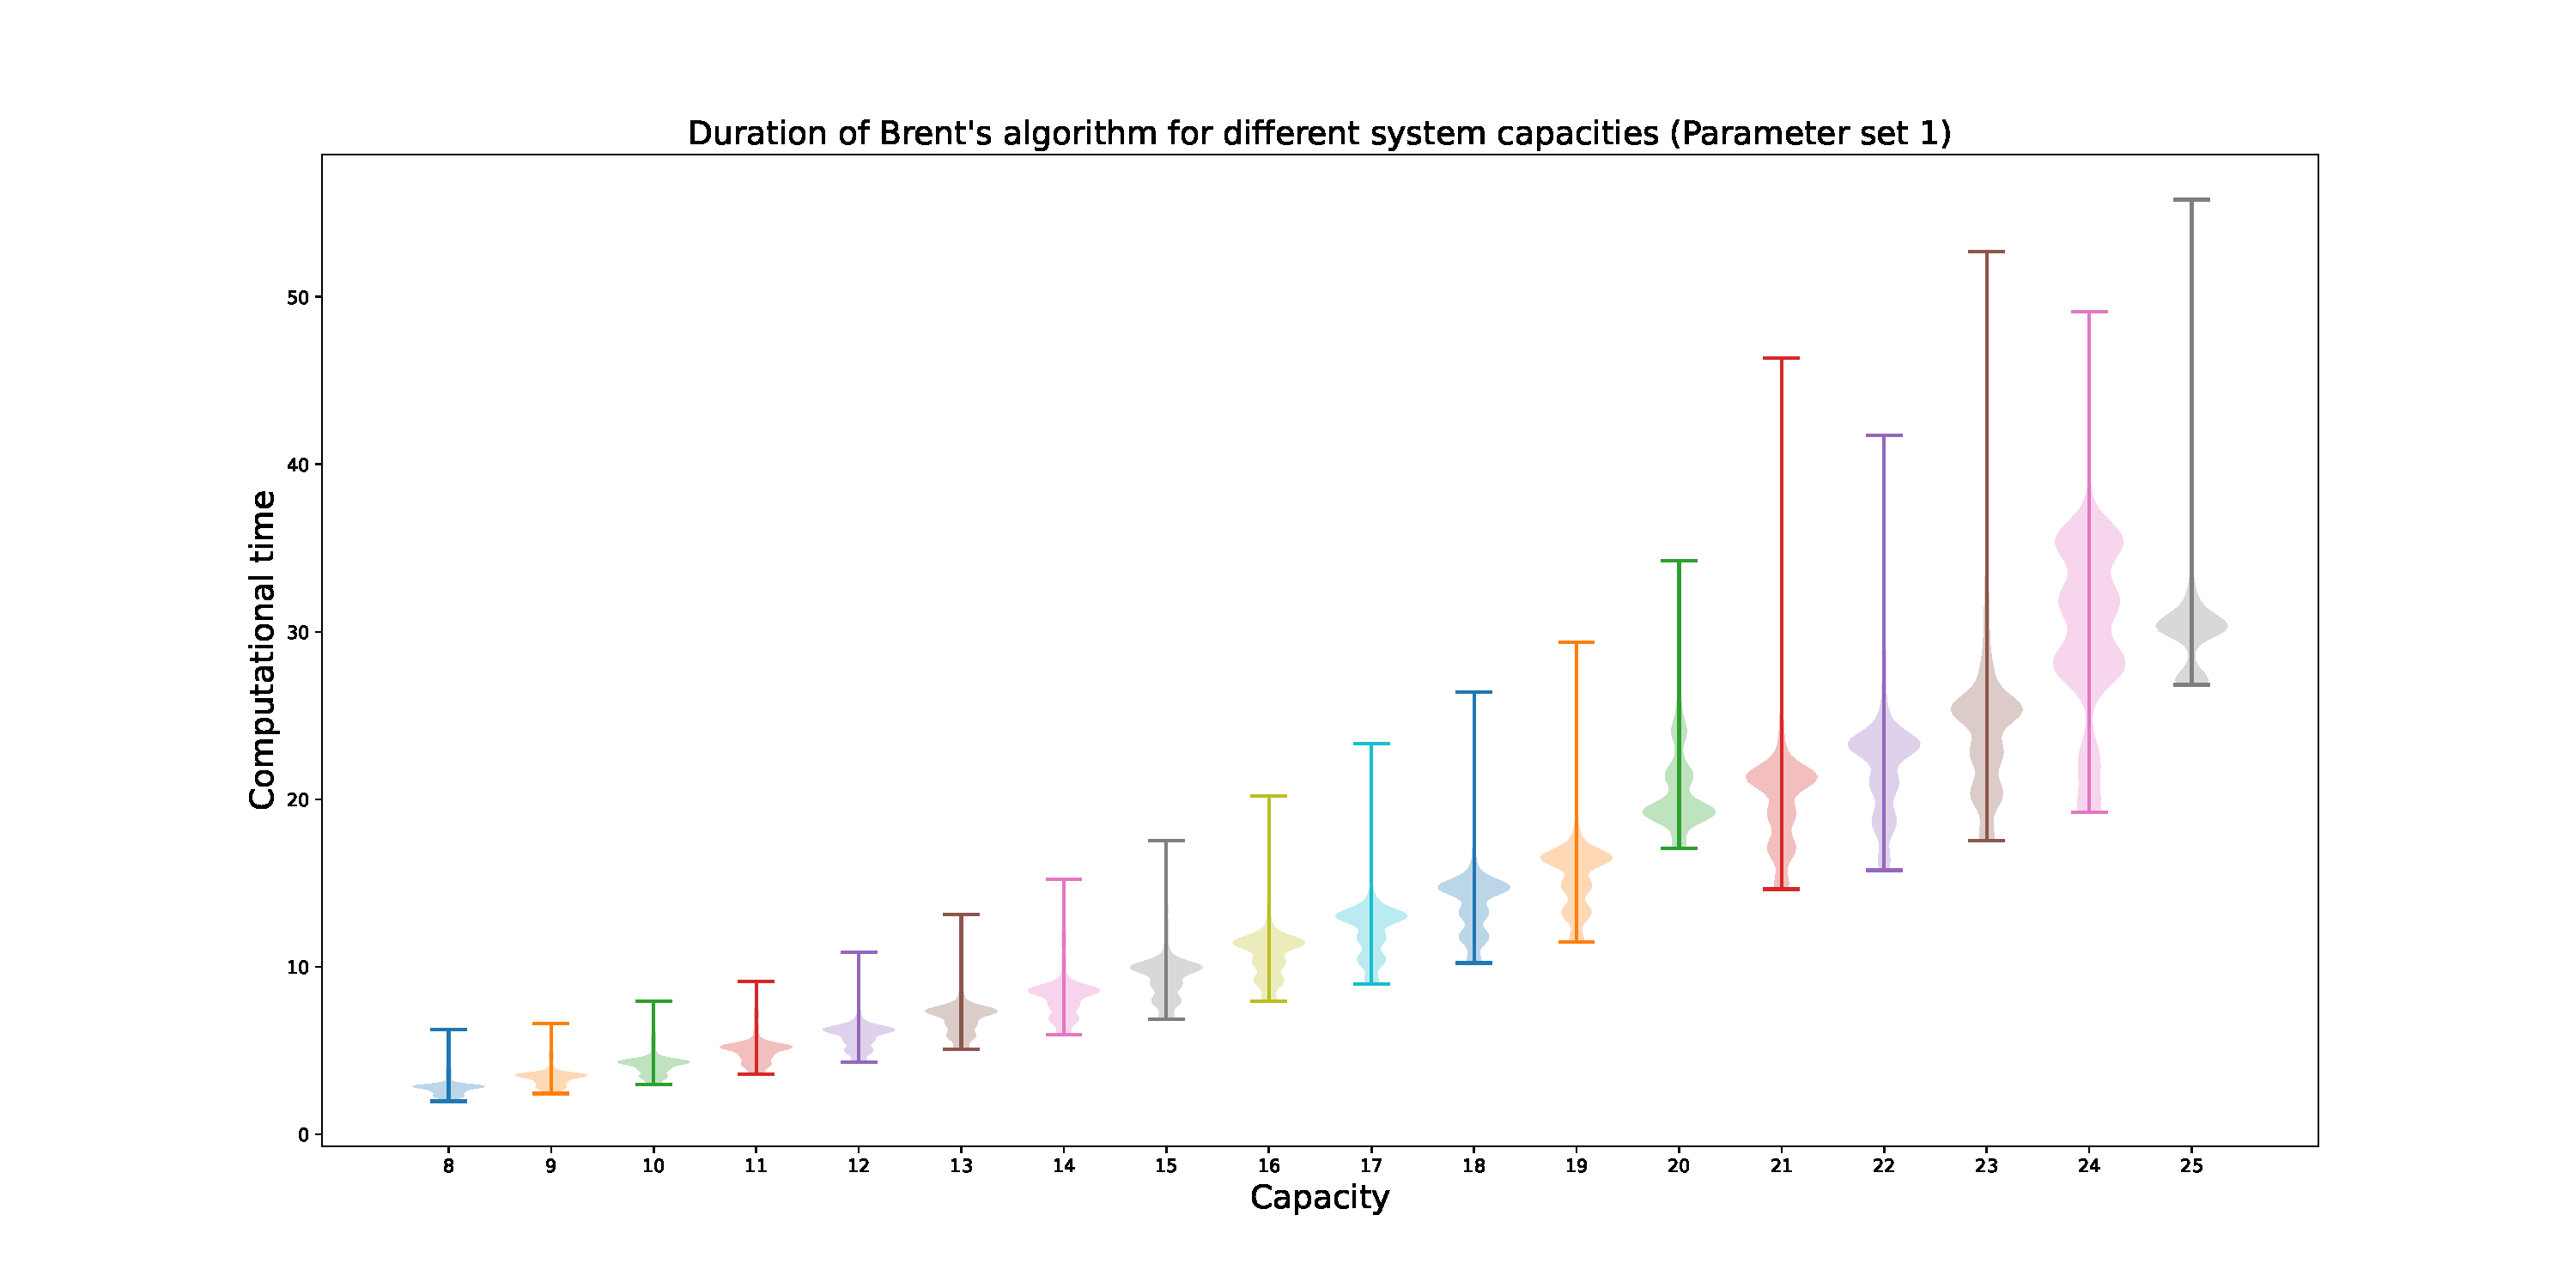
\includegraphics[width=\textwidth]{chapters/04_game_theoretic_model/img/brents_method/tolerance/tolerance_violinplots_1.pdf}
    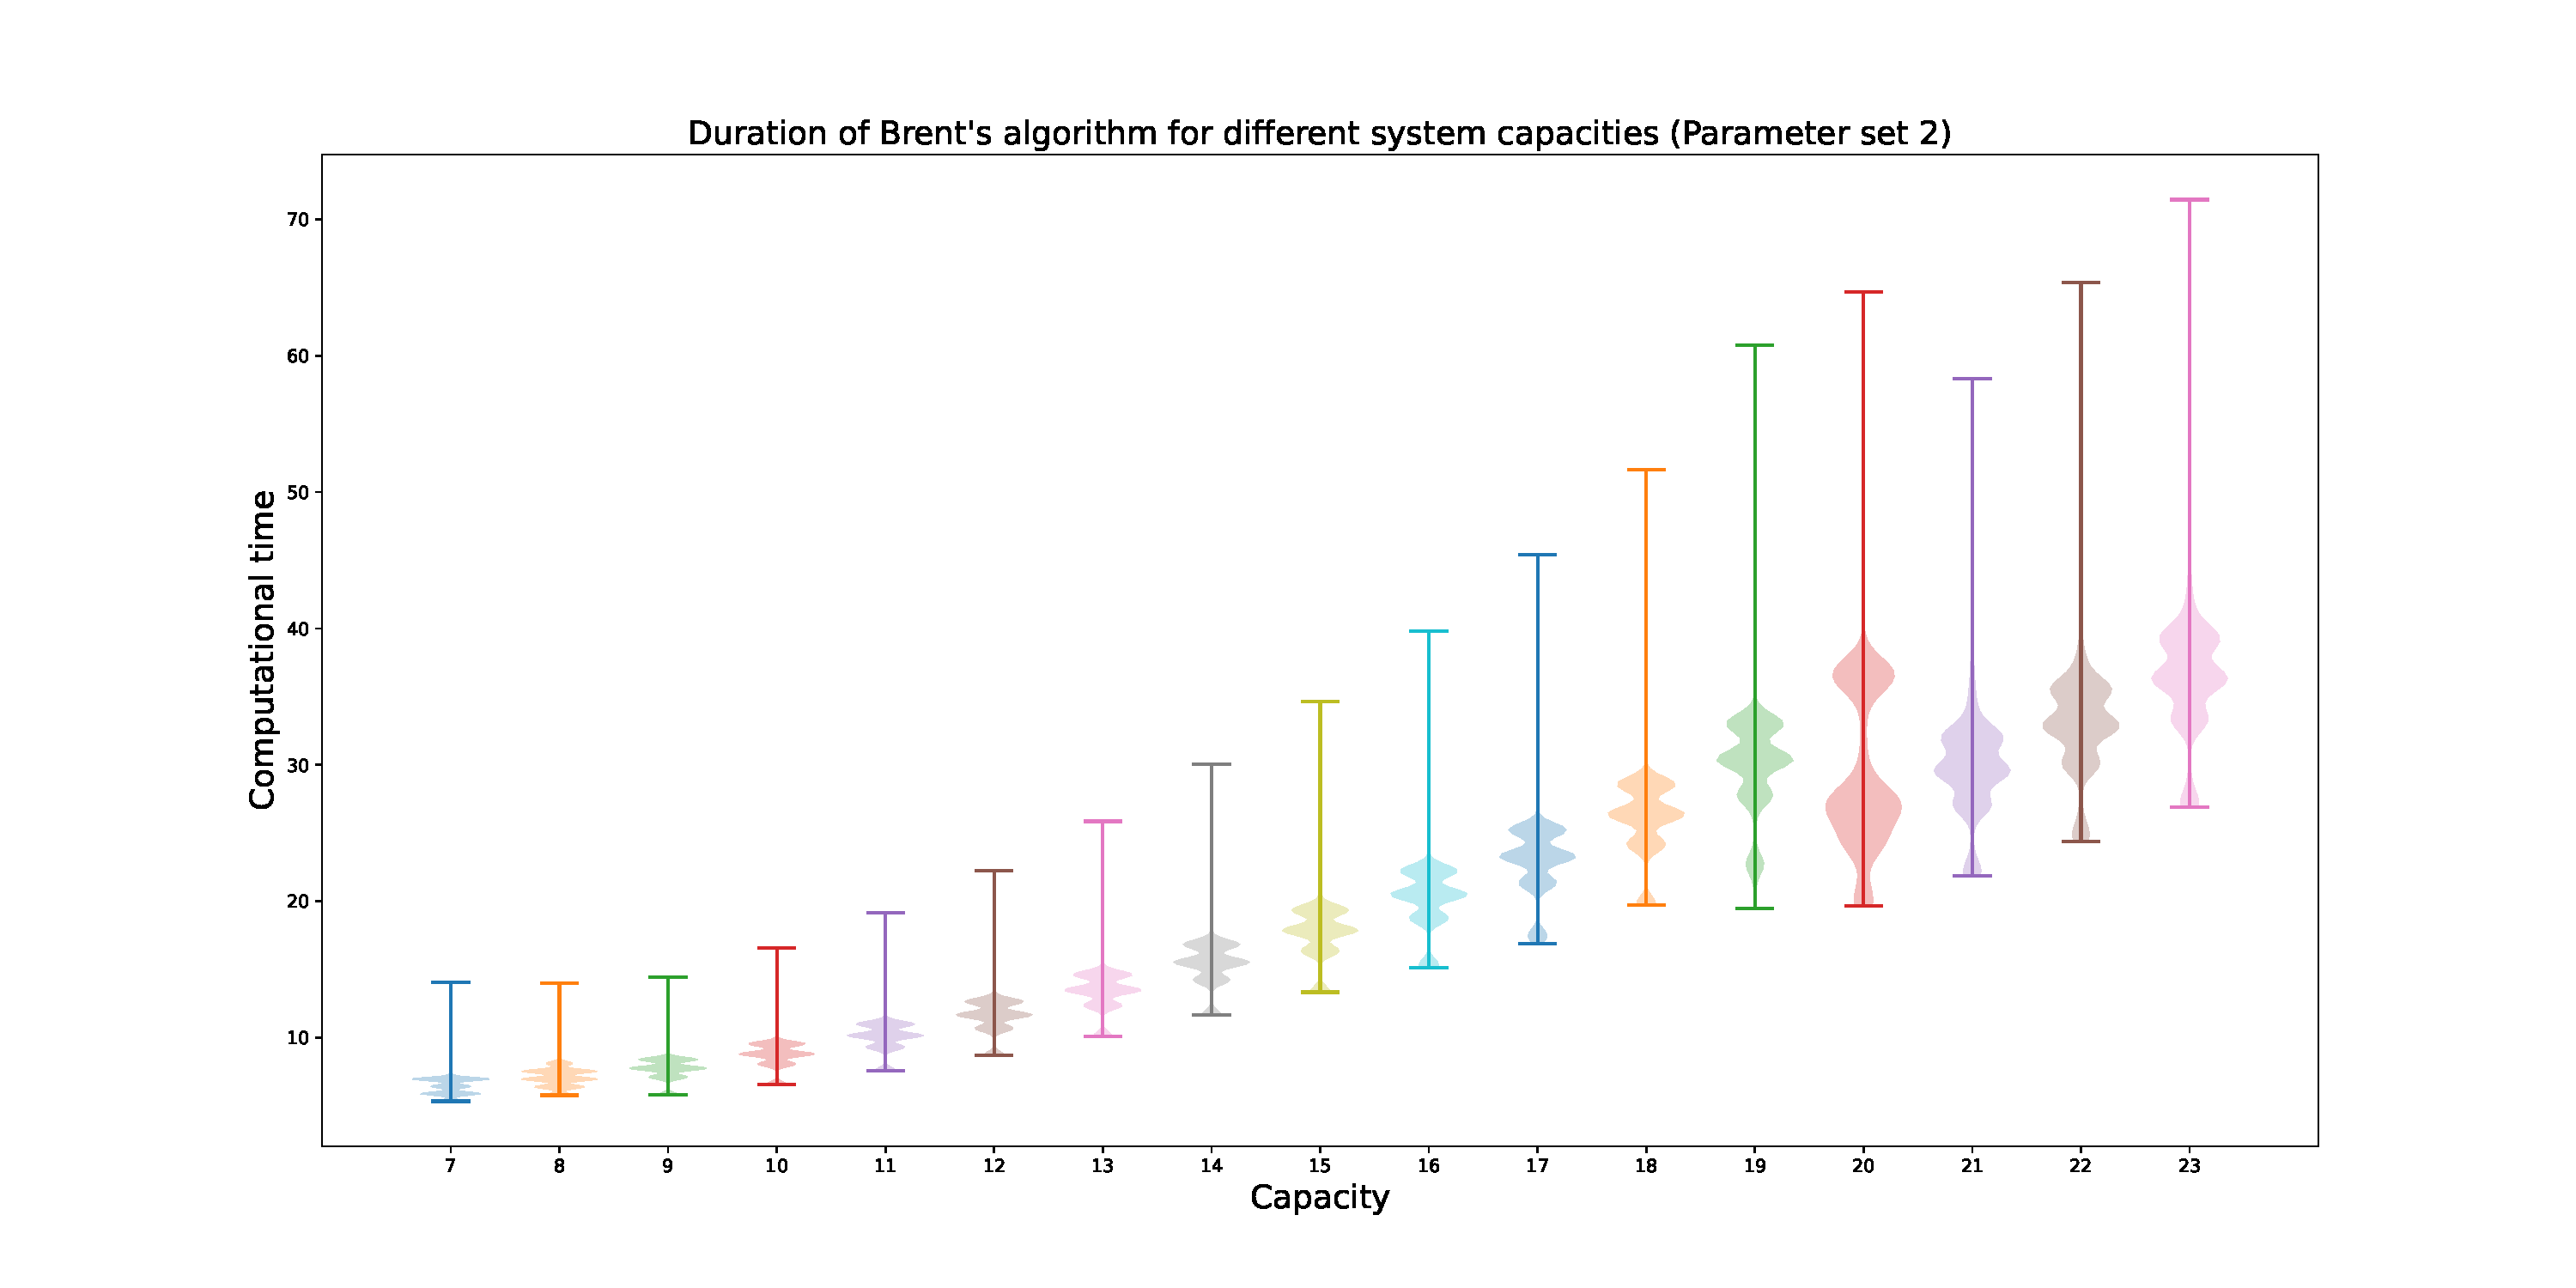
\includegraphics[width=\textwidth]{chapters/04_game_theoretic_model/img/brents_method/tolerance/tolerance_violinplots_2.pdf}
    \caption{
        Violinplots of the duration of Brent's algorithm for different values of
        \(N_A\).
    }
    \label{fig:tolerance_violinplots}
\end{figure}

It can be seen that for both parameter sets in
Figure~\ref{fig:tolerance_violinplots} the duration of the algorithm is
increasing as \(N^A\) increases.
Note that the violinplots include all values of the tolerance parameters
\lstinline[style=pystyle]{xtol} that were used.

\begin{figure}[H]
    \centering
    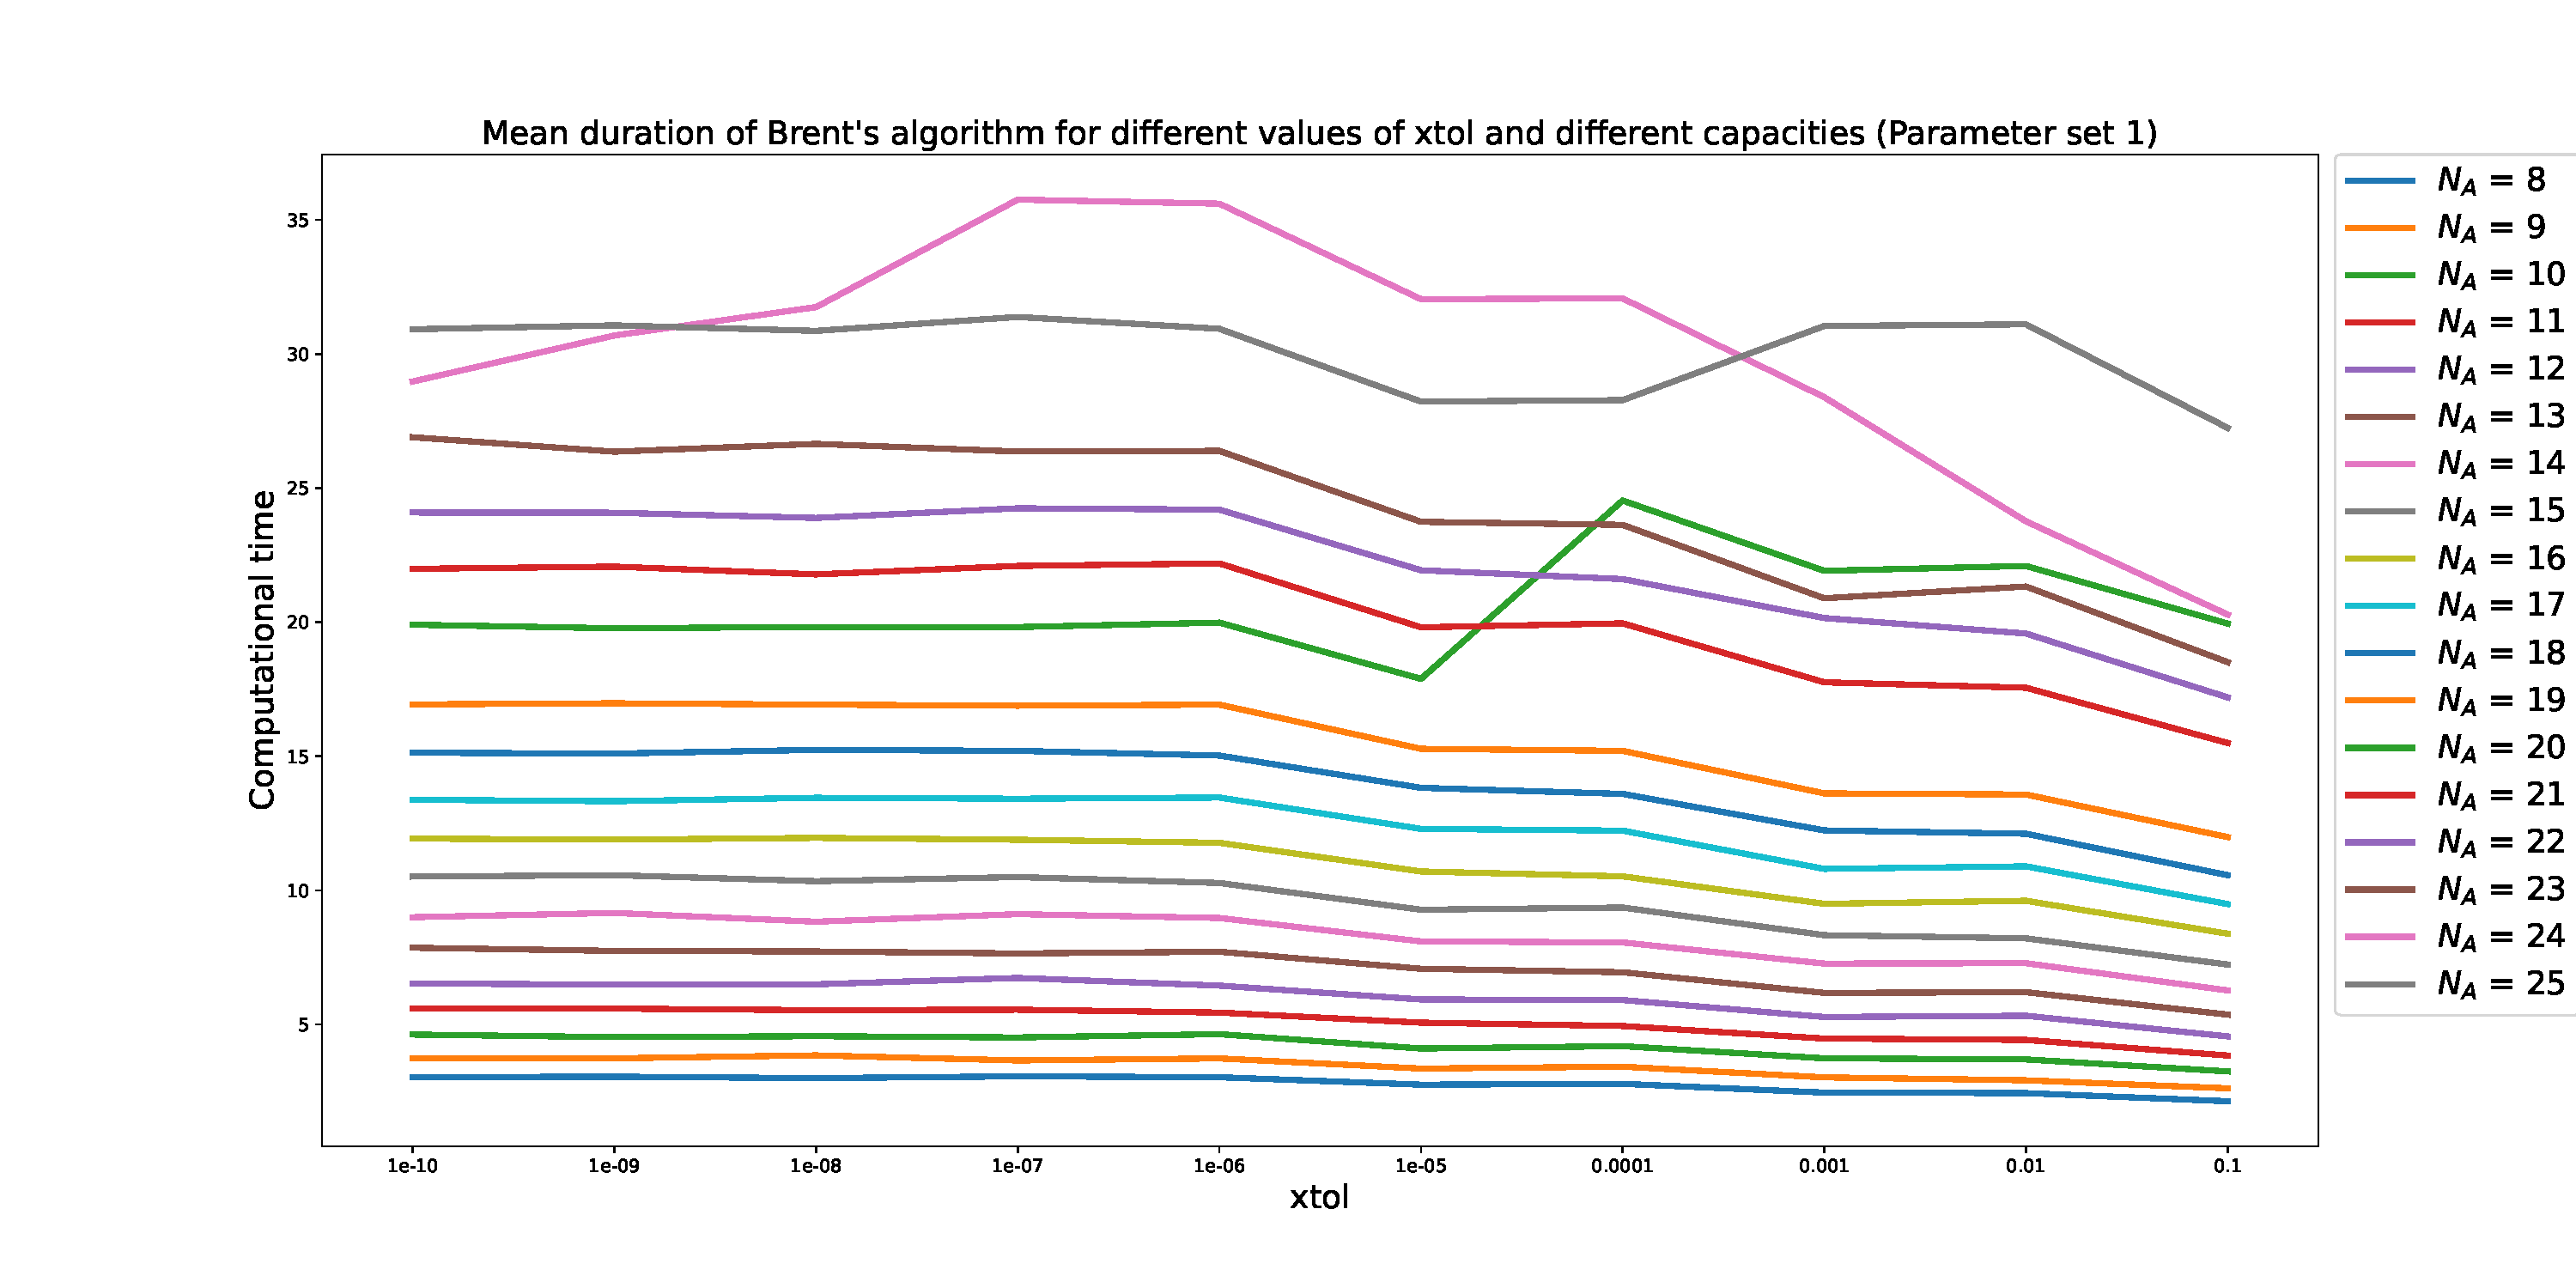
\includegraphics[width=\textwidth]{chapters/04_game_theoretic_model/img/brents_method/tolerance/tolerance_lineplots_1.pdf}
    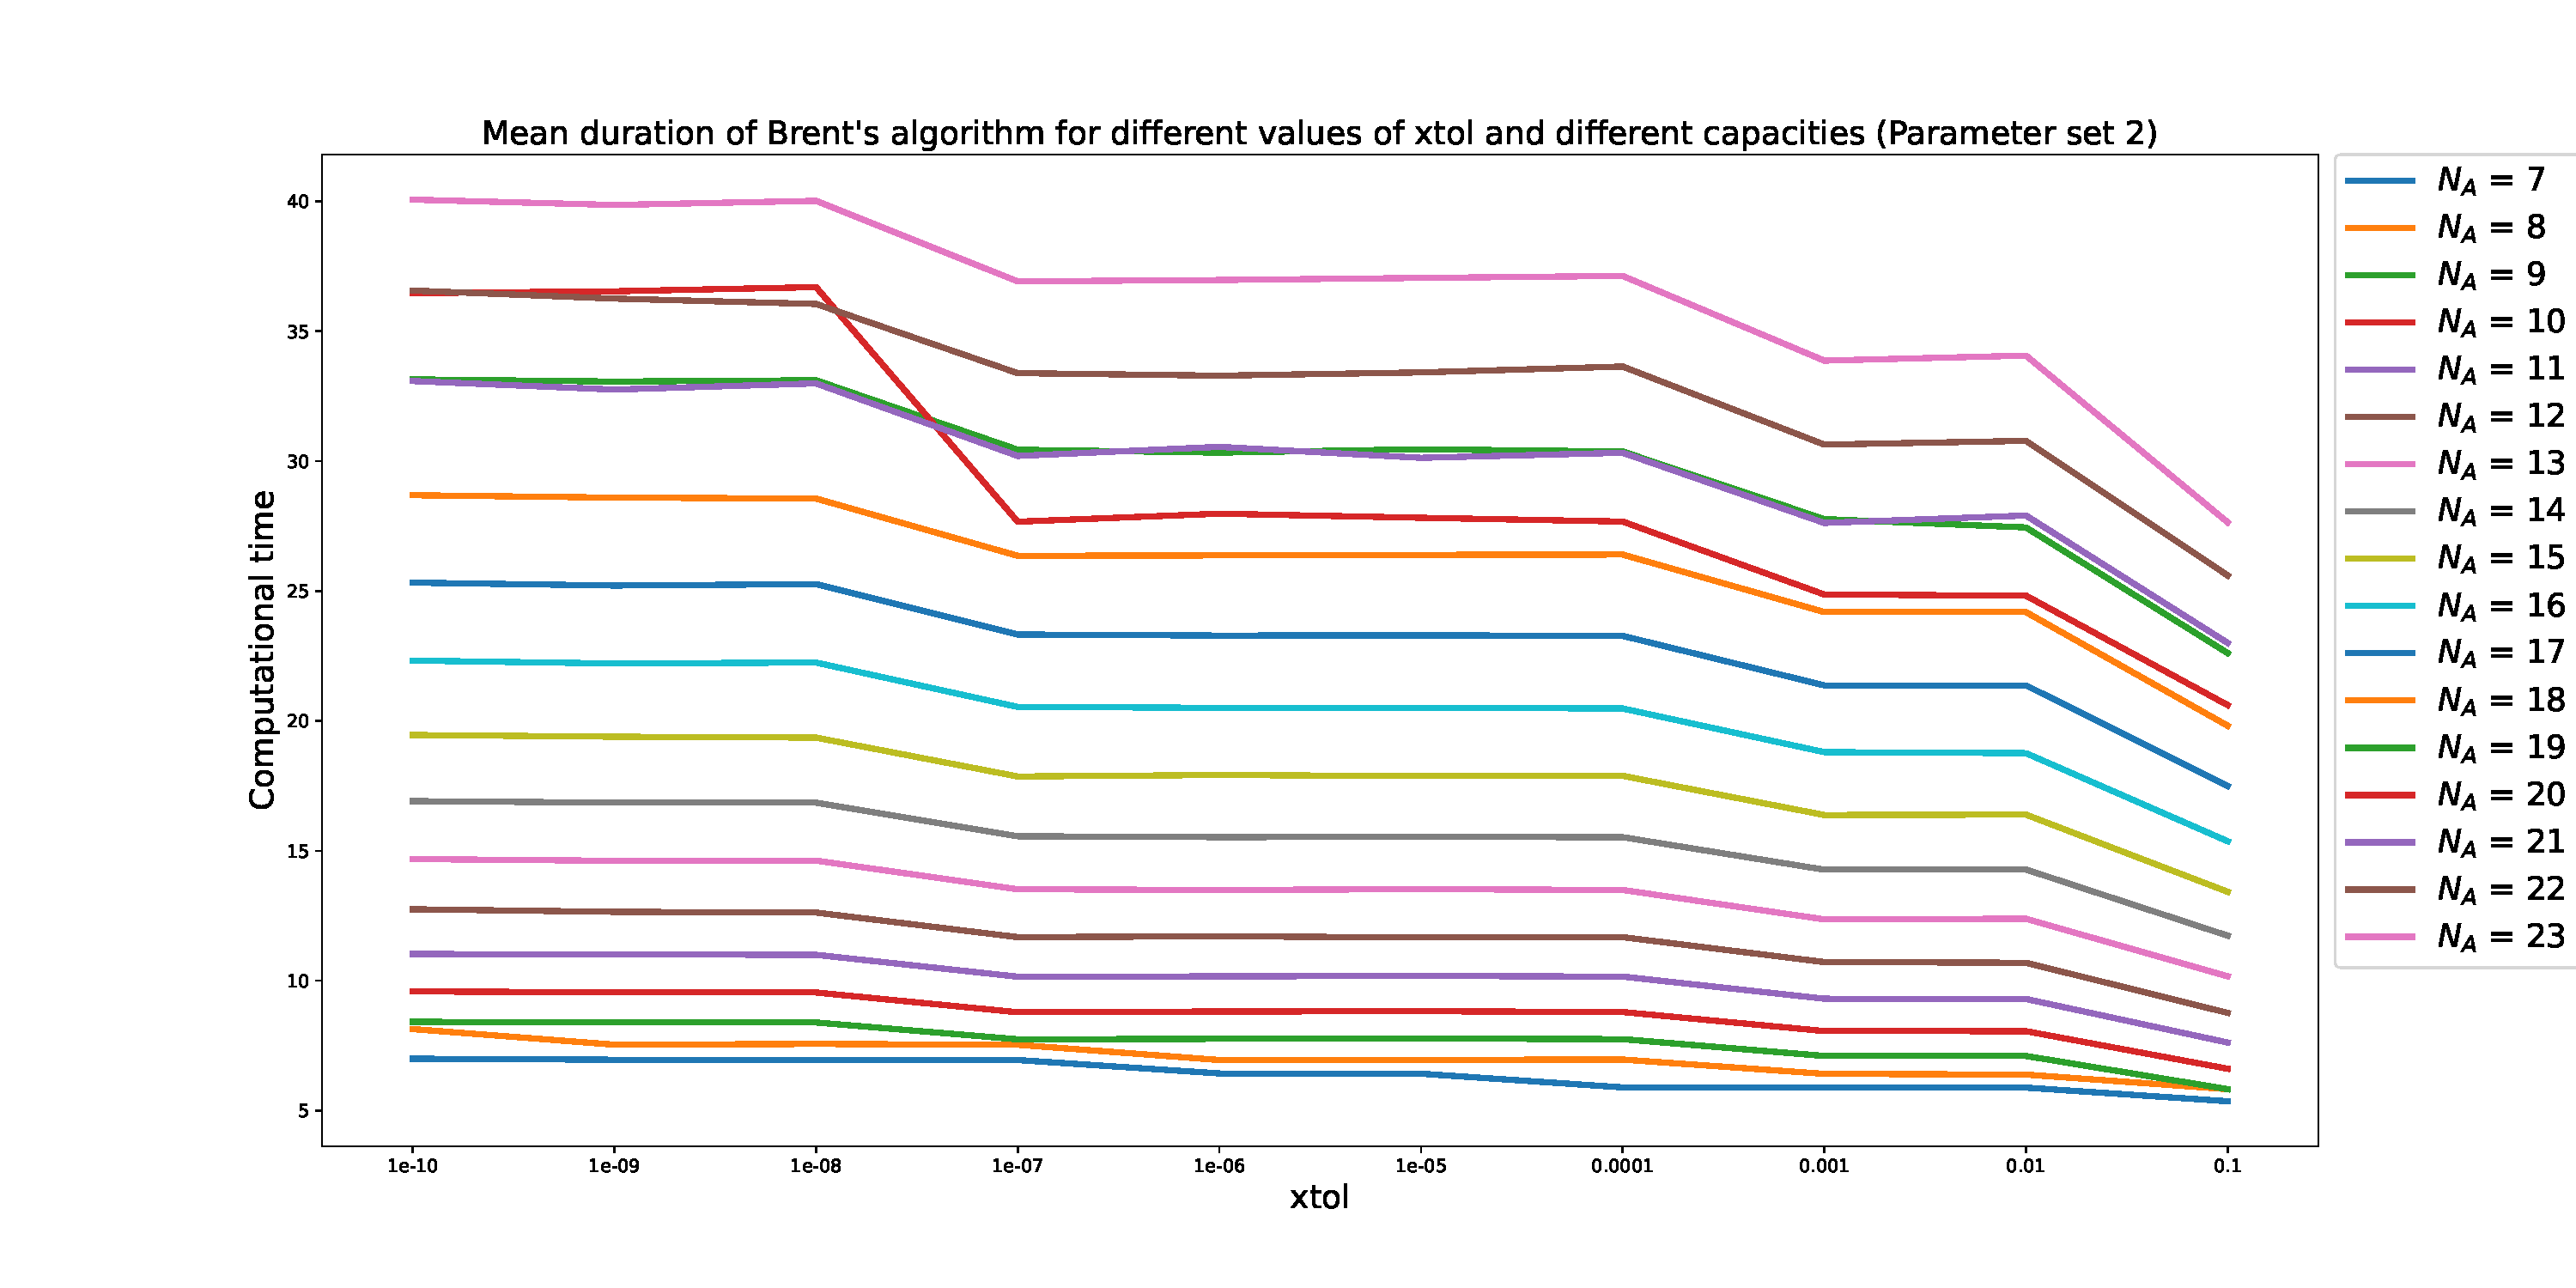
\includegraphics[width=\textwidth]{chapters/04_game_theoretic_model/img/brents_method/tolerance/tolerance_lineplots_2.pdf}
    \caption{
        Line plots of the duration of Brent's algorithm for different values of
        \(N_A\) over different values of the absolute tolerance parameter xtol.
    }
    \label{fig:tolerance_lineplots}
\end{figure}

The plots of Figure~\ref{fig:tolerance_lineplots} show for each value of \(N^A\)
how the duration of the algorithm changes as the absolute tolerance parameter
\lstinline[style=pystyle]{xtol} increases.
It can be seen that for both parameter sets the duration of the algorithm
on most cases the computational time decreases as the tolerance parameter
increases.
There are some cases that do not follow this trend though.
For example, for parameter set 1 when \(N^A=20\), the duration of the algorithm
increases, rather than decreasing, from \lstinline[style=pystyle]{xtol=1e-05}
to \lstinline[style=pystyle]{xtol=0.0001}.



\subsection{Queueing systems and normal form games}
\label{sec:queueing_systems_and_normal_form_games}

In subsection~\ref{sec:best_response_distribution_service} it is shown that
given the strategies played by queueing systems \(A\) and \(B\) the best
response of the distribution service can be found.
Consider the routing matrix \(R\) defined in equation~(\ref{eq:routing_matrix}).

\begin{equation*}
    R =
    \begin{pmatrix}
        p_{1,1}^A & p_{1,2}^A & \dots & p_{1,N_B}^A \\
        p_{2,1}^A & p_{2,2}^A & \dots & p_{2,N_B}^A \\
        \vdots & \vdots & \ddots & \vdots \\
        p_{N_A,1}^A & p_{N_A,2}^A & \dots & p_{N_A,N_B}^A \\
    \end{pmatrix}
\end{equation*}

Every entry \(R_{i,j}\) of the routing matrix represents best response of
the distribution service when \(T^A=i\) and \(T^B=j\).
In other words, given \(T^A=i\) and \(T^B=j\), the distribution service's
strategy that maximises its utility should be to route a proportion of
\(p^A_{i,j}\) of the individuals to queueing system \(A\) and a proportion of
\(1 - p^A_{i,j}\) individuals to queueing system \(B\).
Assuming that for every pair of strategies \(T^A\) and \(T^B\) the best response
of the distribution service is known to the queueing systems, then the
formulation of the game can be simplified even more.
In fact the imperfect information extensive form game defined in
Section~\ref{sec:game_imperfect_information} can be now transformed into a
2-player normal form game between the two queueing systems.
From equation~(\ref{eq:obj_queueing_systems}) the utility of queueing system
\(i\) when the pair of strategies \((T^A, T^B)\) is played, is defined as:

\begin{equation}\label{eq:utility_queueing_systems}
    U_{T_A, T_B}^i = 1 - \left( \hat{P} - P(W_i < t) \right)^2
    \qquad i \in {A, B}
\end{equation}

\(U_{T_A, T_B}^A\) and \(U_{T_A, T_B}^B\) are essentially artificial metrics
that queuing systems \(A\) and \(B\) aim to maximise.
Essentially, by maximising equation~(\ref{eq:utility_queueing_systems}) for both
queueing systems, the queueing systems are trying to minimise the difference
between the proportion of individuals that are served within the target time
\(t\) and the proportion target \(\hat{P}\).
For example, given a proportion target \(\hat{P} = 0.9\) which means that
90\% of the individuals should be served within the target time \(t\), and
given that the proportion of individuals that are served within the target time
is \(P(W_i < t) = 0.8\), then the utility of the queueing system \(i\) is
given by \(U_{T_A, T_B}^i = 1 - (0.9 - 0.8)^2 = 0.99\).
The payoff matrices of the game can be populated by these utilities for all
possible pairs of strategies \((T^A, T^B)\).

\begin{equation}\label{eq:payoff_matrices}
    A =
    \begin{pmatrix}
        U_{1,1}^A & U_{1,2}^A & \dots & U_{1,N_B}^A \\
        U_{2,1}^A & U_{2,2}^A & \dots & U_{2,N_B}^A \\
        \vdots & \vdots & \ddots & \vdots \\
        U_{N_A,1}^A & U_{N_A,2}^A & \dots & U_{N_A,N_B}^A \\
    \end{pmatrix}, \,
    B =
    \begin{pmatrix}
        U_{1,1}^B & U_{1,2}^B & \dots & U_{1,N_B}^B \\
        U_{2,1}^B & U_{2,2}^B & \dots & U_{2,N_B}^B \\
        \vdots & \vdots & \ddots & \vdots \\
        U_{N_A,1}^B & U_{N_A,2}^B & \dots & U_{N_A,N_B}^B \\
    \end{pmatrix}
\end{equation}

Matrix \(A\) consists of all possible utilities of queueing system \(A\), and
matrix \(B\) consists of all possible utilities of queueing system \(B\).
The game is now a 2-player normal form game with payoff matrices \(A\) and
\(B\).


\subsubsection{Implementation}

Consider an example of the described game with the following parameters:

\begin{table}[H]
    \caption{Distribution service parameters}
    \begin{center}
        \begin{tabular}{||c|c|c|c||}
            \hline
            \(\lambda_2\) & t & \(p_A\) & \(\alpha\) \\
            \hline\hline
            4 & 2 & 0.5 & 0.2 \\
            \hline
        \end{tabular}
    \end{center}
    \label{tab:implemetation_dist_service_parameters}
\end{table}

\begin{table}[H]
    \caption{Queueing systems parameters}
    \begin{center}
        \begin{tabular}{||c|c|c|c|c|c||}
            \hline
            \(\lambda_1^A\) & \(\mu^A\) & \(C^A\) & \(N^A\) & \(M^A\) \\
            \hline
            2 & 3 & 2 & 7 & 6 \\
            \hline
        \end{tabular}

        \vspace{0.5cm}
        
        \begin{tabular}{||c|c|c|c|c|c||}
            \hline
            \(\lambda_1^B\) & \(\mu^B\) & \(C^B\) & \(N^B\) & \(M^B\) \\
            \hline
            1 & 1 & 3 & 4 & 3 \\
            \hline
        \end{tabular}
    \end{center}
    \label{tab:implemetation_queueing_systems_parameters}
\end{table}


\begin{lstlisting}[style=pystyle]
>>> lambda_2 = 4
>>> target = 2
>>> p_A = 0.5
>>> alpha = 0.2
>>> 
>>> lambda_1_A = 2
>>> mu_A = 3
>>> num_of_servers_A = 2
>>> system_capacity_A = 7
>>> buffer_capacity_A = 6
>>> 
>>> lambda_1_B = 1
>>> mu_B = 1
>>> num_of_servers_B = 3
>>> system_capacity_B = 4
>>> buffer_capacity_B = 3

\end{lstlisting}

The first function to create is one that takes a pair of thresholds \(T^A=i,
T^B=j\) and gets the best response of the distribution service \(p_A\).
Then, using \(p_A\), finds the value of \(U_{i,j}^A\) and \(U_{i,j}^B\)
and returns the tuple \((i, j, p_A, U_{i,j}^A, U_{i,j}^B)\).

\begin{lstlisting}[style=pystyle]
>>> import numpy as np
>>> def get_individual_entries_of_matrices(
...     lambda_2,
...     lambda_1_1,
...     lambda_1_2,
...     mu_1,
...     mu_2,
...     num_of_servers_1,
...     num_of_servers_2,
...     threshold_1,
...     threshold_2,
...     system_capacity_1,
...     system_capacity_2,
...     buffer_capacity_1,
...     buffer_capacity_2,
...     alpha,
...     target,
...     p_hat=0.95,
... ):
...     """
...     Gets the (i,j)th entry of the payoff matrices and the routing matrix
...     where i=threshold_1 and j=threshold_2. 
...
...     Parameters
...     ----------
...     lambda_2 : float
...     lambda_1_1 : float
...     lambda_1_2 : float
...     mu_1 : float
...     mu_2 : float
...     num_of_servers_1 : int
...     num_of_servers_2 : int
...     threshold_1 : int
...     threshold_2 : int
...     system_capacity_1 : int
...     system_capacity_2 : int
...     buffer_capacity_1 : int
...     buffer_capacity_2 : int
...     alpha : float
...     target : float
...
...     Returns
...     -------
...     tuple
...         A tuple of the form (i, j, R[i,j], A[i,j], B[i,j])
...     """
...     prop_to_hospital_1 = calculate_class_2_individuals_best_response(
...         lambda_2=lambda_2,
...         lambda_1_1=lambda_1_1,
...         lambda_1_2=lambda_1_2,
...         mu_1=mu_1,
...         mu_2=mu_2,
...         num_of_servers_1=num_of_servers_1,
...         num_of_servers_2=num_of_servers_2,
...         system_capacity_1=system_capacity_1,
...         system_capacity_2=system_capacity_2,
...         buffer_capacity_1=buffer_capacity_1,
...         buffer_capacity_2=buffer_capacity_2,
...         threshold_1=threshold_1,
...         threshold_2=threshold_2,
...         alpha=alpha,
...     )
...     prop_to_hospital_2 = 1 - prop_to_hospital_1
... 
...     proportion_within_target_1 = (
...         abg.markov.proportion_within_target_using_markov_state_probabilities(
...             lambda_2=lambda_2 * prop_to_hospital_1,
...             lambda_1=lambda_1_1,
...             mu=mu_1,
...             num_of_servers=num_of_servers_1,
...             threshold=threshold_1,
...             system_capacity=system_capacity_1,
...             buffer_capacity=buffer_capacity_1,
...             class_type=None,
...             target=target,
...         )
...     )
...     proportion_within_target_2 = (
...         abg.markov.proportion_within_target_using_markov_state_probabilities(
...             lambda_2=lambda_2 * prop_to_hospital_2,
...             lambda_1=lambda_1_2,
...             mu=mu_2,
...             num_of_servers=num_of_servers_2,
...             threshold=threshold_2,
...             system_capacity=system_capacity_2,
...             buffer_capacity=buffer_capacity_2,
...             class_type=None,
...             target=target,
...         )
...     )
...     utility_1 = 1 - (
...         (np.nanmean(proportion_within_target_1) - p_hat) ** 2
...     )
...     utility_2 = 1 - (
...         (np.nanmean(proportion_within_target_2) - p_hat) ** 2
...     )
... 
...     return (
...         threshold_1,    
...         threshold_2,
...         prop_to_hospital_1,
...         utility_1,
...         utility_2
...     )

\end{lstlisting}

The function \lstinline[style=pystyle]{get_individual_entries_of_matrices} can
now be used to get the \((i,j)^\text{th}\) entry of the routing matrix \(R\)
payoff matrix \(A\) and payoff matrix \(B\).
For example consider the case when \(T_A = 7\) and \(T_B = 4\).
The equivalent values of \(R, A \text{ and } B\) on the \((7, 4)^\text{th}\)
position can be calculated using:

\begin{lstlisting}[style=pystyle]
>>> _, _, p_A, U_A, U_B = np.round(get_individual_entries_of_matrices(
...     lambda_2=lambda_2,
...     lambda_1_1=lambda_1_A,
...     lambda_1_2=lambda_1_B,
...     mu_1=mu_A,
...     mu_2=mu_B,
...     num_of_servers_1=num_of_servers_A,
...     num_of_servers_2=num_of_servers_B,
...     threshold_1=7,
...     threshold_2=4,
...     system_capacity_1=system_capacity_A,
...     system_capacity_2=system_capacity_B,
...     buffer_capacity_1=buffer_capacity_A,
...     buffer_capacity_2=buffer_capacity_B,
...     alpha=alpha,
...     target=1,
...     p_hat=0.95
... ), 8)
>>> p_A
0.80583153
>>> U_A
0.96146225
>>> U_B
0.87505776

\end{lstlisting}

The second step is to use the
\lstinline[style=pystyle]{get_individual_entries_of_matrices} function to
calculate the entries of the routing matrix \(R\), payoff matrix \(A\) and
payoff matrix \(B\).
Thus, by iterating over all possible values of \(T_A\) and \(T_B\), the
routing matrix \(R\), payoff matrix \(A\) and payoff matrix \(B\) can be
calculated.
Note that in Section~\ref{sec:implementation_distribution_service} the
\lstinline[style=pystyle]{get_routing_matrix} function was defined that returns
the routing matrix \(R\).
The function defined here gets all matrices in a much more computationally
efficient way.

\begin{lstlisting}[style=pystyle]
>>> import itertools
>>> def get_payoff_matrices(
...     lambda_2,
...     lambda_1_1,
...     lambda_1_2,
...     mu_1,
...     mu_2,
...     num_of_servers_1,
...     num_of_servers_2,
...     system_capacity_1,
...     system_capacity_2,
...     buffer_capacity_1,
...     buffer_capacity_2,
...     target,
...     alternative_utility=False,
...     alpha=0,
... ):
...     """
...     The function uses the distribution array (that is the array that holds the
...     optimal proportion of individuals to send to each hospital), to calculate
...     the proportion of patients within time for every possible set of thresholds
...     chosen by each system.
...     Parameters
...     ----------
...     lambda_2 : float
...     lambda_1_1 : float
...     lambda_1_2 : float
...     mu_1 : float
...     mu_2 : float
...     num_of_servers_1 : int
...     num_of_servers_2 : int
...     system_capacity_1 : int
...     system_capacity_2 : int
...     buffer_capacity_1 : int
...     buffer_capacity_2 : int
...     target : float
...         The target time that individuals should be within
...
...     Returns
...     -------
...     numpy.array, numpy.array
...         The payoff matrices of the game
...     """
...     utility_matrix_1 = np.zeros((system_capacity_1, system_capacity_2))
...     utility_matrix_2 = np.zeros((system_capacity_1, system_capacity_2))
...     routing_matrix = np.zeros((system_capacity_1, system_capacity_2))
...     for threshold_1, threshold_2 in itertools.product(
...         range(1, system_capacity_1 + 1), range(1, system_capacity_2 + 1)
...     ):
...         T_A, T_B, p_A, U_A, U_B = get_individual_entries_of_matrices(
...             lambda_2=lambda_2,
...             lambda_1_1=lambda_1_1,
...             lambda_1_2=lambda_1_2,
...             mu_1=mu_1,
...             mu_2=mu_2,
...             num_of_servers_1=num_of_servers_1,
...             num_of_servers_2=num_of_servers_2,
...             threshold_1=threshold_1,
...             threshold_2=threshold_2,
...             system_capacity_1=system_capacity_1,
...             system_capacity_2=system_capacity_2,
...             buffer_capacity_1=buffer_capacity_1,
...             buffer_capacity_2=buffer_capacity_2,
...             alpha=alpha,
...             target=target,
...         )
...         utility_matrix_1[T_A - 1, T_B - 1] = U_A
...         utility_matrix_2[T_A - 1, T_B - 1] = U_B
...         routing_matrix[T_A - 1, T_B - 1] = p_A
...
...     return utility_matrix_1, utility_matrix_2, routing_matrix
        
\end{lstlisting}
    
The following piece of code gets matrices \(A\), \(B\) and \(R\) for the
parameters of the example given above.

\begin{lstlisting}[style=pystyle]
>>> A, B, R = get_payoff_matrices(
...     lambda_2=lambda_2,
...     lambda_1_1=lambda_1_A,
...     lambda_1_2=lambda_1_B,
...     mu_1=mu_A,
...     mu_2=mu_B,
...     num_of_servers_1=num_of_servers_A,
...     num_of_servers_2=num_of_servers_B,
...     system_capacity_1=system_capacity_A,
...     system_capacity_2=system_capacity_B,
...     buffer_capacity_1=buffer_capacity_A,
...     buffer_capacity_2=buffer_capacity_B,
...     target=target,
...     alpha=0,
... )
>>> A
array([[0.99783349, 0.99783349, 0.99783349, 0.99783349],
       [0.99791294, 0.997908  , 0.9978956 , 0.99788205],
       [0.99818675, 0.99815898, 0.9980942 , 0.99803223],
       [0.99858555, 0.99852554, 0.99838075, 0.99824713],
       [0.99908345, 0.99899654, 0.99875599, 0.99853094],
       [0.99953429, 0.99946954, 0.99917061, 0.99886562],
       [0.99962588, 0.99962588, 0.99947103, 0.9991795 ]])
>>> B
array([[0.99199207, 0.99157153, 0.98986388, 0.98018693],
       [0.99199207, 0.99176915, 0.99047978, 0.98403475],
       [0.99199207, 0.99180175, 0.99065167, 0.98526931],
       [0.99199207, 0.99183129, 0.99080081, 0.98623919],
       [0.99199207, 0.99186433, 0.99095294, 0.98711709],
       [0.99199207, 0.99192113, 0.99117199, 0.98816358],
       [0.99199207, 0.99199207, 0.99166644, 0.9899607 ]])
>>> R
array([[0.92992288, 0.44649026, 0.23605342, 0.12099486],
       [1.        , 0.8562699 , 0.62075404, 0.44170806],
       [1.        , 0.88253463, 0.67740094, 0.51730643],
       [1.        , 0.90410709, 0.72074724, 0.57415867],
       [1.        , 0.92632326, 0.76116766, 0.62524083],
       [1.        , 0.96104926, 0.81485397, 0.68749328],
       [1.        , 1.        , 0.92669791, 0.80590018]])

\end{lstlisting}

The final thing to be done is to use the \lstinline[style=pystyle]{nashpy}
library to build the game using the payoff matrices.

\begin{lstlisting}[style=pystyle]
>>> import nashpy as nash
>>> game = nash.Game(A, B)
>>> game
Bi matrix game with payoff matrices:
<BLANKLINE>
Row player:
[[0.99783349 0.99783349 0.99783349 0.99783349]
 [0.99791294 0.997908   0.9978956  0.99788205]
 [0.99818675 0.99815898 0.9980942  0.99803223]
 [0.99858555 0.99852554 0.99838075 0.99824713]
 [0.99908345 0.99899654 0.99875599 0.99853094]
 [0.99953429 0.99946954 0.99917061 0.99886562]
 [0.99962588 0.99962588 0.99947103 0.9991795 ]]
<BLANKLINE>
Column player:
[[0.99199207 0.99157153 0.98986388 0.98018693]
 [0.99199207 0.99176915 0.99047978 0.98403475]
 [0.99199207 0.99180175 0.99065167 0.98526931]
 [0.99199207 0.99183129 0.99080081 0.98623919]
 [0.99199207 0.99186433 0.99095294 0.98711709]
 [0.99199207 0.99192113 0.99117199 0.98816358]
 [0.99199207 0.99199207 0.99166644 0.9899607 ]]

\end{lstlisting}



\subsection{Solving the game}\label{sec:game_solving}

For a 2-player game once the two payoff matrices have been calculated
the game can be solved using the methods described in this section.
There are two concepts that will be used to analyse the behavioural patterns
of the players in the game; the Nash equilibrium and Evolutionary Stable
Strategies.


\section{ED-EMS application}\label{sec:game_ems_ed_application}

Similar to Section~\ref{sec:queueing_ems_ed_application}, the game theoretic
model can be applied to the same healthcare setting.
All concepts described in this Section can be mapped to some components of
either the ED or the EMS.

The EMS has to decide how to distribute its patients among the two EDs so that
the weighted combination of the ambulance blocking time and the percentage of
lost ambulances is minimised.
This can be illustrated by figure \ref{fig:diagram_of_game_theoretic_model}.
The interaction between the two
EDs is a normal form game that is then used to inform the decision of the EMS.
Note that the formulated game here assumes that prior to making a choice the
EMS knows the strategies that each ED is playing (figure
\ref{fig:imperfect_info_game}).
This corresponds to reacting to experienced delays.

The queueing systems of the hospitals are designed in such a way where they can
accept two types of individuals (section \ref{sec:queueing_section}).
Each hospital may then choose to block type 2 individuals
when the hospital reaches a certain capacity.
The strategy sets for each hospital is the set
\( \{T \in \mathbb{N} \;|\; 1 \leq T \leq N\} \) where \(N \in\{N_A, N_B\}\) are
the total capacities of hospitals \(A\) and \(B\).
The chosen actions from the strategy set are denoted as \(T_A, T_B\) and are
the \textit{thresholds}.

Both hospitals follow a queueing model with two waiting spaces for
individuals.
The first waiting space (i.e. the waiting space of the hospital) is where the
patients queue right before receiving
their service and has a queue capacity of \( N - C \), where \(N\) is the total
capacity of the hospital and \(C\) is the number of healthcare
professionals able to see them.
The second waiting space (i.e. the parking space for ambulances) is where
ambulances, that are sent from the
EMS distributor, stay until their patients are allowed to enter the hospital.
The parking space has a capacity of \(M\) and no servers.
This is shown diagrammatically in Figure~\ref{fig:diagram_of_queueing_system}.

Note here that both types of individuals can become lost to the system.
An individual allocated from the ambulance service becomes lost to the system
whenever
an arrival occurs and the parking space is at full capacity (\(M\)
ambulances already parked).
Similarly, type \(1\) individuals get lost whenever they arrive at the waiting
space of the hospital and it is at full capacity (\(N - C\) individuals already
waiting).

There are certain assumptions that are made in this application.
Firstly, it is assumed that the distance from any patient's location to any
hospital is not a factor that will affect the EMS's decision.
That means that under the scope of this application, the EMS does not have to
consider the closest hospital to the patient's location.
Secondly, it is assumed that a patient's timer (from the perspective of the ED)
does not start counting until the patient enters the hospital.
For instance, consider the case where a patient is sent from the EMS to hospital
\(A\) and is blocked in the parking space of hospital \(A\) for \(6\) hours.
The patient then proceeds to wait in the hospital for an additional \(2\) hours
and is then receiving their treatment for \(1\) hour.
The patient's total time in the hospital is assumed to be \(3\) hours (\(2+1\)).
Finally, the last assumption that is made is that arrival and service times are
exponentially distributed.

